\chapter{Physical Implementations}

\section{Analytic Solvers}

\glc\ typically solves the system of \glspl{ode} which describe the evolution of a galaxy using a numerical solver. However, in some situations analytic solutions may be available. \glc\ allows for the use of analytic solvers in such cases. Currently available analytic solvers are described below.

\subsection{Simple Disk Satellites}

This solver, which can be activated by setting {\normalfont \ttfamily [diskVerySimpleUseAnalyticSolver]}$=${\normalfont \ttfamily true} is applicable to satellite systems in the very simple disk component. In particular, the following conditions must be met for it to be valid:
\begin{itemize}
\item The hot halo component must be of type {\normalfont \ttfamily verySimple} or {\normalfont \ttfamily verySimpleDelayed};
\item The satellite component must be of type {\normalfont \ttfamily verySimple};
\item The disk component must be of type {\normalfont \ttfamily verySimple};
\item Properties of all other components must not change for satellite galaxies (with the exception of the {\normalfont \ttfamily time} property of the basic component), or else the component must be {\normalfont \ttfamily null};
  \item Disk star formation and outflow rates must scale as $M_{\rm gas}/\tau$ where $M_{\rm gas}$ is the instantaneous mass of gas in the galaxy disk, and $\tau$ is a fixed timescale for any given satellite galaxy.
\end{itemize}
Under these conditions, the flow of mass between gas, stellar, and outflowed phases is analytically solvable.

\section{Accretion of Gas into Halos}\label{sec:AccretionBaryonic}\index{accretion!baryonic}

The accretion rate of gas from the \gls{igm} into a dark matter halo is expected to depend on (at least) the rate at which that halo mass is growing, the depth of its potential well and the thermodynamical properties of the accreting gas. \glc\ implements the following calculations of gas accretion from the \gls{igm}, which can be selected via the {\normalfont \ttfamily accretionHaloMethod} input parameter.

\subsection{Simple}\label{phys:accretionHalo:accretionHaloSimple}

Selected using {\normalfont \ttfamily accretionHaloMethod}$=${\normalfont \ttfamily simple}, this method sets the accretion rate of baryons into a halo to be:
\begin{equation}
 \dot{M}_{\mathrm accretion} = \left\{ \begin{array}{ll} (\Omega_{\mathrm b}/\Omega_{\mathrm M}) \dot{M}_{\mathrm halo} & \hbox{ if } V_{\mathrm virial} > V_{\mathrm reionization} \hbox{ or } z > z_{\mathrm reionization} \\ 0 & \hbox{ otherwise,}\end{array} \right.
\label{eq:accretionHalo:truncation}
\end{equation}
where $z_{\mathrm reionization}=${\normalfont \ttfamily [reionizationSuppressionRedshift]} is the redshift at which the Universe is reionized and $V_{\mathrm reionization}=${\normalfont \ttfamily [reionizationSuppressionVelocity]} is the virial velocity below which accretion is suppressed after reionization. Setting $V_{\mathrm reionization}$ to zero will effectively switch off the effects of reionization on the accretion of baryonics. This algorithm attempts to offer a simple prescription for the effects of reionization and has been explored by multiple authors (e.g. \citealt{benson_effects_2002}). In particular, \cite{font_modelingmilky_2010} show that it produces results in good agreement with more elaborate treatments of reionization. For halos below the accretion threshold, any accretion rate that would have otherwise occurred is instead placed into the ``failed'' accretion rate. For halos which can accrete, and which have some mass in their ``failed'' reservoir, that mass will be added to the regular accretion rate at a rate equal to the mass of the 
``failed'' reservoir times the specific growth rate of the halo. The gas accreted is assumed to be from a pristine \gls{igm} and so has zero abundances. Chemical abundances are computed from the chemical state functions (see \S\ref{sec:ChemicalStateMethod}).

Note that, if $\dot{M}_{\mathrm halo} < 0$ then negative accretion rates of gas into the node can result. This ccan be prevented by setting {\normalfont \ttfamily [accretionHalosSimpleNegativeAccretionAllowed]}$=${\normalfont \ttfamily false}.

By default, gas is accreted whenever the halo is growing in total mass. However, setting {\normalfont \ttfamily [accretionHalosSimpleAccreteNewGrowthOnly]}$=${\normalfont \ttfamily true} causes accretion to occur only if the node mass is growing and exceeds the previous maximum node mass achieved along this branch of the merger tree. This requires use of a basic component which tracks the maximum mass along the branch (i.e. the {\normalfont \ttfamily massMaximum} property).

\subsection{Null}\label{phys:accretionHalo:accretionHaloNull}

Selected using {\normalfont \ttfamily accretionHaloMethod}$=${\normalfont \ttfamily null}, this method sets the accretion rate of baryons into a halo to be zero always.

\subsection{Cold Mode}\label{phys:accretionHalo:accretionHaloColdMode}

Selected using {\normalfont \ttfamily accretionHaloMethod}$=${\normalfont \ttfamily coldMode}, this class extends the {\normalfont \ttfamily simple} class by dividing the accretion into hot and cold mode components. The cold mode fraction follows the approximation introduced by \cite{benson_cold_2010}, namely:
\begin{equation}
f_{\mathrm cold}=(1+r^{1/\delta})^{-1},
\end{equation}
where $\delta=${\normalfont \ttfamily [accretionColdModeShockStabilityTransitionWidth]}, $r = \epsilon_{\mathrm crit}/\epsilon$, and
\begin{equation}
\epsilon = r_{\mathrm s} \Lambda / \rho_{\mathrm s} v_{\mathrm s}^3,
\end{equation}
where $r_{\mathrm s}$ is the accretion shock radius, $\Lambda$ is the post-shock cooling function, $\rho_{\mathrm s}$ is the pre-shock density, $v_{\mathrm s}$ is the pre-shock velocity, and $\epsilon_{\mathrm crit}=${\normalfont \ttfamily [accretionColdModeShockStabilityThreshold]}. The pre-shock radius is set equal to the halo virial radius, the pre-shock velocity is set equal to the halo virial velocity, while the pre-shock density is given by
\begin{equation}
\rho_{\mathrm s} = {\gamma - 1 \over \gamma + 1} { 3 \over 4 \pi } { \Omega_{\mathrm b} \over \Omega_{\mathrm m} } {M \over r_{\mathrm s}^3} \left[ 1 + {(\alpha + 3) (10 + 9 \pi) \over 4} \right]^{-1},
\end{equation}
where $M$ is the total halo mass, $\gamma(=5/3)$ is the adiabatic index of the gas, and $\alpha$ is the exponent of the initial power-law density perturbation ($\alpha=0$ is assumed). The post-shock density and temperature are found assuming the strong-shock limit.

\subsection{Bertschinger}\label{phys:accretionHalo:accretionHaloBertschinger}

Selected using {\normalfont \ttfamily accretionHaloMethod}$=${\normalfont \ttfamily bertschinger}, this class extends the {\normalfont \ttfamily simple} class by replacing the total halo mass and accretion rate with the Bertschinger (i.e. turnaround) mass and its rate of increase respectively. Additionally, truncation of accretion (eqn.~\ref{eq:accretionHalo:truncation}) is determined by the maximum circular velocity of the node rather than by the virial velocity.

\section{Cosmology Functions}\index{cosmology}

The background cosmology describes the evolution of an isotropic, homoegeneous Universe within which our calculations are carried out. For the purposes of \glc, the background cosmology is used to relate expansion factor/redshift to cosmic time and to compute the density of various components (e.g. dark matter, dark energy, etc.) at different epochs. Background cosmological models are specified via the {\normalfont \ttfamily cosmologyMethod}, and the physics that must be implemented for each cosmological model is describe in more detail in \S\ref{sec:methodsCosmologyFunctions}. Currently implemented cosmological models are as follows.

\subsection{Matter + Lambda}\label{phys:cosmologyFunctions:cosmologyFunctionsMatterLambda}

Selected with {\normalfont \ttfamily cosmologyMethod}$=${\normalfont \ttfamily matter-lambda}, in this implementation cosmological relations are computed assuming a universe that contains only collisionless matter and a cosmological constant.

\subsection{Matter + Dark Energy}\label{phys:cosmologyFunctions:cosmologyFunctionsMatterDarkEnergy}\index{dark energy}

Selected with {\normalfont \ttfamily cosmologyMethod}$=${\normalfont \ttfamily matter-darkEnergy}, in this implementation cosmological relations are computed assuming a universe that contains only collisionless matter and dark energy with an equation of state $w(a)=w_0+w_1a(1-a)$ \citep{jassal_wmap_2005}, with $w_0=${\normalfont \ttfamily [darkEnergyEquationOfStateW0]}, and $w_1=${\normalfont \ttfamily [darkEnergyEquationOfStateW1]}.

\section{Circumnuclear Accretion Disks}\label{sec:CircumnuclearDisks}\index{accretion disks}\index{accretion!disk}

Circumnuclear accretion disks surrounding supermassive black holes at the centers of galaxies influence the evolution of both the black hole (via accretion rates of mass and angular momentum and possibly by extracting rotational energy from the black hole) and the surrounding galaxy if they lead to energetic outflows (e.g. jets) from the nuclear region. Accretion disk type is specified via the {\normalfont \ttfamily accretionDisksMethod}, and the physics that must be implemented for each accretion disk type is describe in more detail in \S\ref{sec:AccretionDisks}. Current implementations of accretion disks are as follows.

\subsection{Shakura-Sunyaev Geometrically Thin, Radiatively Efficient Disks}

Selected with {\normalfont \ttfamily accretionDisksMethod}$=${\normalfont \ttfamily Shakura-Sunyaev}, this implementation assumes that accretion disks are always described by a radiatively efficient, geometrically thin accretion disk as described by \cite{shakura_black_1973}. The radiative efficiency of the flow is computed assuming that material falls into the black hole without further energy loss from the \gls{isco}, while the spin-up rate of the black hole is computed assuming that the material enters the black hole with the specific angular momentum of the \gls{isco} (i.e. there are no torques on the material once it begins to fall in from the \gls{isco}; \citealt{bardeen_kerr_1970}). For these thin disks, jet power is computed, using the expressions from \citeauthor{meier_association_2001}~(\citeyear{meier_association_2001}; his equations 4 and 5).

\subsection{Advection Dominated, Geometrically Thick, Radiatively Inefficient Flows (ADAFs)}

Selected with {\normalfont \ttfamily accretionDisksMethod}$=${\normalfont \ttfamily ADAF}, this implementation assumes that accretion is via an \gls{adaf} \citep{narayan_advection-dominated_1994} which is radiatively inefficient and geometrically thick. The radiative efficiency of the flow, which will be zero for a pure \gls{adaf}, is controlled by {\normalfont \ttfamily [adafRadiativeEfficiencyType]}. If set to {\normalfont \ttfamily fixed}, then the radiative efficiency is set to the value of the input parameter {\normalfont \ttfamily [adafRadiativeEfficiency]}. Alternatively, if set to {\normalfont \ttfamily thinDisk} the radiative efficiency will be set to that of a Shakura-Sunyaev thin disk. The spin up rate of the black hole and the jet power produced as material accretes into the black hole are computed using the method of \cite{benson_maximum_2009}. The maximum efficiency of the jet (in units of the accretion power $\dot{M} {\mathrm c}^2$) is set by {\normalfont \ttfamily [adafJetEfficiencyMaximum]}---in the model of \cite{benson_maximum_2009} the jet efficiency diverges as $j\rightarrow 1$, setting a maximum 
is important to avoid numerical instabilities. The energy of the accreted material can be set equal to the energy at infinity (as expected for a pure \gls{adaf}) or the energy at the \gls{isco} by use of the {\normalfont \ttfamily [adafEnergyOption]} parameter (set to {\normalfont \ttfamily pureADAF} or {\normalfont \ttfamily ISCO} respectively). The \gls{adaf} structure is controlled by the adiabatic index, $\gamma$, and viscosity parameter, $\alpha$, which are specified via the {\normalfont \ttfamily [adafAdiabaticIndex]} and {\normalfont \ttfamily [adafViscosityOption]} input parameters respectively. The field-enhancing shear, $g$, is computed using $g=\exp(\omega \tau)$ if {\normalfont \ttfamily [adafFieldEnhanceType]} is set to ``exponential'' where $\omega$ is the frame-dragging frequency and $\tau$ is the smaller of the radial inflow and azimuthal velocity timescales. If  {\normalfont \ttfamily [adafFieldEnhanceType]} is set to ``linear'' then the alternative version, $g=1+\omega \tau$ is used instead. {\normalfont \ttfamily [adafViscosityOption]} may be set to ``{\normalfont \ttfamily fit}'', in which case the fitting function for $\alpha$ as a function of black hole 
spin is used:
\begin{eqnarray}
\alpha(j)=0.015+0.02 j^4 & \hbox{ if  }& g=\exp(\omega\tau) \hbox{ and } E=E_{\mathrm ISCO}, \\
\alpha(j)=0.025+0.08 j^4 & \hbox{ if } & g=1+\omega\tau \hbox{ and } E=E_{\mathrm ISCO}, \\
\alpha(j)=0.010+0.00 j^4 & \hbox{ if } & g=\exp(\omega\tau) \hbox{ and } E=1, \\
\alpha(j)=0.025+0.02 j^4 & \hbox{ if } & g=1+\omega\tau \hbox{ and } E=1.  
\end{eqnarray}

\subsection{``Switched'' Disks}

Selected with {\normalfont \ttfamily accretionDisksMethod}$=${\normalfont \ttfamily switched}, this method allows for accretion disks to switched between radiatively efficient (Shakura-Sunyaev) and inefficient (\gls{adaf}) modes. The properties of the switched disk (e.g. radiative efficiency, jet power), are a linear combination of those of the Shakura-Sunyaev and \gls{adaf} modes, with the \gls{adaf} fraction being given by:
\begin{equation}
f_{\mathrm ADAF} = [1+\exp(y_{\mathrm min})]^{-1} + [1+\exp(y_{\mathrm max})]^{-1},
\label{eq:SwitchedDiskADAFFraction}
\end{equation}
where
\begin{eqnarray}
y_{\mathrm min} &=& +\log(x/x_{\mathrm min})/\Delta_{x}, \\
y_{\mathrm max} &=& -\log(x/x_{\mathrm max})/\Delta_{x},
\end{eqnarray}
and,
\begin{equation}
x = \dot{M} / \dot{M}_{\mathrm Eddington}.
\end{equation}
Here, $x_{\mathrm min}=${\normalfont \ttfamily [accretionRateThinDiskMinimum]}, $x_{\mathrm max}=${\normalfont \ttfamily [accretionRateThinDiskMaximum]}, and $\Delta_{x}$={\normalfont \ttfamily [accretionRateTransitionWidth]}. If either {\normalfont \ttfamily [accretionRateThinDiskMinimum]} or {\normalfont \ttfamily [accretionRateThinDiskMaximum]} is set to ``{\normalfont \ttfamily none}'' then the corresponding term in eqn.~(\ref{eq:SwitchedDiskADAFFraction}) is excluded.

Additionally, if {\normalfont \ttfamily [accretionDiskSwitchedScaleAdafRadiativeEfficiency]} is set to {\normalfont \ttfamily true} then the radiative efficiency of the \gls{adaf} component is reduced by a factor $x/x_{\mathrm min}$ when $x<x_{\mathrm min}$.

\subsection{Eddington-limited Disks}

Selected with {\normalfont \ttfamily accretionDisksMethod}$=${\normalfont \ttfamily eddingtonLimited}, this method does not assume any physical model for the accretion disk, but merely assumes that jets are powered at a fixed fraction {\normalfont \ttfamily [accretionDiskJetPowerEddington]} of the Eddington luminosity. The radiative efficiency is similarly set at a fixed value of {\normalfont \ttfamily [accretionDiskRadiativeEfficiencyEddington]}. Since no physical model for the disk is assumed, the black hole spin up rate is always set to zero.

\section{Dark Matter Structure Formation}\index{structure formation}\index{dark matter}

A variety of functions are used to describe structure formation in dark matter dominated universes. These are described below.

\subsection{Primordial Power Spectrum}\label{sec:PrimordialPowerSpectrum}\index{power spectrum!primordial}

The functional form of the primordial dark matter power spectrum is selected via the {\normalfont \ttfamily powerSpectrumMethod} parameter. The power spectrum is computed from the specified primordial power spectrum and the transfer function (see \S\ref{sec:TransferFunction}) and normalized to a value of $\sigma_8$ specified by {\normalfont \ttfamily [sigma\_8]}.

\subsubsection{(Running) Power Law Spectrum}

Selected via {\normalfont \ttfamily powerSpectrumMethod}$=${\normalfont \ttfamily powerLaw}, this method implements a primordial power spectrum of the form:
\begin{equation}
 P(k) \propto k^{n_{\mathrm eff}(k)},
\end{equation}
where
\begin{equation}
 n_{\mathrm eff}(k) = n_{\mathrm s} + {1\over 2}{\d n \over \d \ln k} \ln \left( {k \over k_{\mathrm ref}} \right),
\end{equation}
where $n_{\mathrm s}=${\normalfont \ttfamily powerSpectrumIndex} is the power spectrum index at wavenumber $k_{\mathrm ref}=${\normalfont \ttfamily powerSpectrumReferenceWavenumber} and $\d n / \d \ln k=${\normalfont \ttfamily powerSpectrumRunning} describes the running of this index with wavenumber.

\subsection{Cosmological Mass Root Variance}

The method used to compute the root variance of the cosmological mass field, $\sigma(M)$, is selected via the {\normalfont \ttfamily cosmologicalMassVarianceMethod} parameter.
\subsubsection{Filtered Power Spectrum}

Selected via {\normalfont \ttfamily cosmologicalMassVarianceMethod}$=${\normalfont \ttfamily filteredPowerSpectrum}, this method computes the mass root variance using:
\begin{equation}
 \sigma^2(M) = {1 \over 2 \pi^2} \int_0^\infty P(k) T^2(k) W^2(k) k^2 {\mathrm d}k
\end{equation}
where $P(k)$ is the primordial power spectrum (see \S\ref{sec:PrimordialPowerSpectrum}), $T(k)$ is the transfer function (see \S\ref{sec:TransferFunction}), and $W(k)$ is the power spectrum variance window function (see \S\ref{sec:PowerSpectrumWindowFunctionPhysics}).

\subsection{Power Spectrum Variance Window Function}\label{sec:PowerSpectrumWindowFunctionPhysics}\index{power spectrum!variance}\index{power spectrum!window function}

The functional form of the window function used in computing the variance of the power spectrum is selected via the {\normalfont \ttfamily powerSpectrumWindowFunctionMethod} parameter. Note that when computing the normalization of the power spectrum to match the specified value of $\sigma_8$ a top-hat real-space window function is \emph{always} used (as per the definition of $\sigma_8$).

\subsubsection{Top-hat}

Selected via {\normalfont \ttfamily powerSpectrumWindowFunctionMethod}$=${\normalfont \ttfamily topHat}, this method implements a top-hat window function in real-space:
\begin{equation}
 W(k) = {3 (\sin(x)-x \cos(x)) \over x^3},
\end{equation}
where $x = k R$ and $R=(3M/4\pi\bar{\rho})^{1/3}$ for a smoothing scale $M$ and mean matter density $\bar{\rho}$.

\subsubsection{Sharp in $k$-space}

Selected via {\normalfont \ttfamily powerSpectrumWindowFunctionMethod}$=${\normalfont \ttfamily kSpaceSharp}, this method implements a top-hat window function in $k$-space:
\begin{equation}
 W(k) = \left\{ \begin{array}{ll} 1 & \hbox{if } k < k_{\mathrm s} \\ 0 & \hbox{if } k > k_{\mathrm s}, \end{array} \right.
\end{equation}
where if {\normalfont \ttfamily [powerSpectrumWindowFunctionSharpKSpaceNormalization]}$=${\normalfont \ttfamily natural} then $k_{\mathrm s} = (6 \Pi^2 \bar{\rho} / M)^{1/3}$ for a smoothing scale $M$ and mean matter density $\bar{\rho}$. Otherwise, {\normalfont \ttfamily [powerSpectrumWindowFunctionSharpKSpaceNormalization]} must be set to a numerical value, $\alpha$, in which case $k_{\mathrm s} = \alpha / R_{\mathrm th}$ with $R_{\mathrm th}=3M/4\pi\bar{\rho}$ for a smoothing scale $M$ and mean matter density $\bar{\rho}$.

\subsubsection{Hybrid of Top-hat and Sharp in $k$-space}

Selected via {\normalfont \ttfamily powerSpectrumWindowFunctionMethod}$=${\normalfont \ttfamily topHatKSpaceSharpHybrid}, this method implements a convolution of a top-hat window function and sharp $k$-space window function in $k$-space:
\begin{equation}
 W(k) = W_{\mathrm th}(k) W_{\mathrm s}(k),
\end{equation}
where
\begin{equation}
 W(k) = {3 (\sin(x)-x \cos(x)) \over x^3},
\end{equation}
where $x = k R_{\mathrm th}$, and
\begin{equation}
 W_{\mathrm s}(k) = \left\{ \begin{array}{ll} 1 & \hbox{if } k < k_{\mathrm s} \\ 0 & \hbox{if } k > k_{\mathrm s}, \end{array} \right.
\end{equation}
where $k{\mathrm s} = \alpha / R_{\mathrm s}$ if {\normalfont \ttfamily [powerSpectrumWindowFunctionSharpKSpaceNormalization]} is assigned a numerical value. Alternatively, if {\normalfont \ttfamily [powerSpectrumWindowFunctionSharpKSpaceNormalization]}$=${\normalfont \ttfamily natural} then the value of $\alpha$ is chosen such that $k_{\mathrm s} = (6 \Pi^2 \bar{\rho}/M)^{1/3}$ if $R_{\mathrm s}=3M/4\pi\bar{\rho}$.

The radii, $R_{\mathrm th}$ and $R_{\mathrm s}$, are chosen such that:
\begin{eqnarray}
R_{\mathrm th}^2 + R_{\mathrm s}^2 &=& (3M/4\pi\bar{\rho})^{2/3} \\
R_{\mathrm s} &=& \beta R_{\mathrm th},
\end{eqnarray}
where $\beta=${\normalfont \ttfamily [powerSpectrumWindowFunctionSharpKSpaceTopHatRadiiRatio]}.

\subsection{Non-linear Matter Power Spectrum}\index{power spectrum!non-linear}

The non-linear matter power spectrum method is selected via the {\normalfont \ttfamily powerSpectrumNonlinearMethod} parameter.

\subsubsection{Linear}

Selected via {\normalfont \ttfamily powerSpectrumNonlinearMethod}$=${\normalfont \ttfamily linear}, this method simply returns the linear matter power spectrum. It is intended primarily for testing purposes.

\subsubsection{Peacock \& Dodds (1996)}

Selected via {\normalfont \ttfamily powerSpectrumNonlinearMethod}$=${\normalfont \ttfamily Peacock-Dodds1996}, this method usese the fitting function of \cite{peacock_non-linear_1996} to compute the non-linear matter power spectrum.

\subsubsection{CosmicEmu}

Selected via {\normalfont \ttfamily powerSpectrumNonlinearMethod}$=${\normalfont \ttfamily CosmicEmu}, this method usese the cosmic emulator (``CosmicEmu'') code of \cite{lawrence_coyote_2010} to evaluate the non-linear matter power spectrum. The CosmicEmu code will be downloaded, compiled and run as necessary if this option is utilized.

\subsection{Transfer Function}\label{sec:TransferFunction}\index{transfer function}

The functional form of the cold dark matter transfer function is selected via the {\normalfont \ttfamily transferFunctionMethod} parameter. The power spectrum is computed from the specified transfer function and the primordial power spectrum (see \S\ref{sec:PrimordialPowerSpectrum}) and normalized to a value of $\sigma_8$ specified by {\normalfont \ttfamily [sigma\_8]}.

\subsubsection{Null}

Selected with {\normalfont \ttfamily transferFunctionMethod}$=${\normalfont \ttfamily null}, this method assumes $T(k)=1$ for all $k$.

\subsubsection{BBKS}

Selected with {\normalfont \ttfamily transferFunctionMethod}$=${\normalfont \ttfamily BBKS}, this method uses the fitting function of \cite{bardeen_statistics_1986} to compute the \gls{cdm} transfer function. The BBKS warm dark matter transfer function\index{transfer function!warm dark matter}\index{warm dark matter!transfer function} can be used by specifying the appropriate streaming length (in Mpc) via the {\normalfont \ttfamily [transferFunctionWDMFreeStreamingLength]} parameter.

\subsubsection{Eisenstein \& Hu}

Selected with {\normalfont \ttfamily transferFunctionMethod}$=${\normalfont \ttfamily Eisenstein-Hu1999}, this method uses the fitting function of \cite{eisenstein_power_1999} to compute the \gls{cdm} transfer function. It requires that the effective number of neutrino species be specified via the {\normalfont \ttfamily effectiveNumberNeutrinos} parameter and summed mass of all neutrino species (in eV) be specified via the {\normalfont \ttfamily summedNeutrinoMasses} parameter. Additionally, the transfer function can be modified to model warm dark matter using the fitting function given by \cite{barkana_constraints_2001}:
\begin{equation}
T(k) \rightarrow T(k) (1+[\epsilon k R_{\mathrm c}^0]^{2\nu})^{-\eta/\nu},
\end{equation}
where $R_{\mathrm c}^0=${\normalfont \ttfamily [transferFunctionWdmCutOffScale]}, $\epsilon=${\normalfont \ttfamily [transferFunctionWdmEpsilon]}, $\eta=${\normalfont \ttfamily [transferFunctionWdmEta]}, $\nu=${\normalfont \ttfamily [transferFunctionWdmNu]}.

\subsubsection{{\normalfont \scshape CAMB}}\label{sec:TransferFunction:CAMB}

Selected with {\normalfont \ttfamily transferFunctionMethod}$=${\normalfont \ttfamily CAMB}, this method uses the \href{http://camb.info/}{\normalfont \scshape CAMB} code to compute the \gls{cdm} transfer function. It requires that the mass fraction of helium in the early Universe be specified via the {\normalfont \ttfamily Y\_He} parameter. {\normalfont \scshape CAMB} will be downloaded and run if the transfer function needs to be computed. It will then be stored in a file for future reference.

\subsubsection{File}

Selected with {\normalfont \ttfamily transferFunctionMethod}$=${\normalfont \ttfamily file}, this method reads a tabulated transfer function from an XML file (specified via the {\normalfont \ttfamily transferFunctionFile} parameter), interpolating between tabulated points. The structure of the transfer function file is described in \S\ref{sec:TransferFunctionMethod}.

\subsection{Linear Growth Function}\index{linear growth}

The function describing the amplitude of linear perturbations is selected via the {\normalfont \ttfamily linearGrowthMethod} parameter.

\subsubsection{Simple}

Selected with {\normalfont \ttfamily linearGrowthMethod}$=${\normalfont \ttfamily simple}, this method calculates the growth of linear perturbations using standard perturbation theory in a Universe consisting of matter and a cosmological constant. Perturbations in the baryons are treated just as for dark matter (i.e. pressure forces are ignored), while perturbations in the radiation are assumed not to grow.

\subsection{Critical Overdensity}\label{sec:criticalOverdensityMethod}\index{density!critical}

The method used to compute the critical linear overdensity at which overdense regions virialize is selected via the {\normalfont \ttfamily criticalOverdensityMethod} parameter.

\subsubsection{Spherical Collapse (Matter + Cosmological Constant)}

Selected with {\normalfont \ttfamily criticalOverdensityMethod}$=${\normalfont \ttfamily sphericalTopHat} this method calculates critical overdensity using a spherical top-hat collapse model assuming a Universe which contains matter and a cosmological constant (see, for example, \citealt{percival_cosmological_2005}).

\subsubsection{Kitayama \& Suto (1996)}

Selected with {\normalfont \ttfamily criticalOverdensityMethod}$=${\normalfont \ttfamily Kitayama-Suto1996} this method calculates critical overdensity using the fitting formula of \cite{kitayama_semianalytic_1996}, and so is valid only in flat cosmological models (an error will be reported in non-flat models). Specifically,
\begin{equation}
 \delta_{\mathrm crit} (t) = {3 (12 \pi)^{2/3} \over 20} [1 + 0.0123 \log_{10}\left\{\Omega_{\mathrm matter}(t)\right\}]/D(t).
\end{equation}

\subsubsection{Fixed}

Selected with {\normalfont \ttfamily criticalOverdensityMethod}$=${\normalfont \ttfamily fixed} this method sets the critical overdensity equal to a fixed value (set via the parameter {\normalfont \ttfamily [criticalOverdensityFixed]}) divided by the linear growth factor.

\subsection{Critical Overdensity Mass Scaling}\index{critical density!mass scaling}

The method used to compute the scaling with mass of the critical linear overdensity at which overdense regions virialize is selected via the {\normalfont \ttfamily criticalOverdensityMassScalingMethod} parameter.

\subsubsection{Null}

Selected with {\normalfont \ttfamily criticalOverdensityMassScalingMethod}$=${\normalfont \ttfamily null} this method assumes that the critical overdensity is independent of mass.

\subsubsection{Warm Dark Matter}

Selected with {\normalfont \ttfamily criticalOverdensityMassScalingMethod}$=${\normalfont \ttfamily warmDarkMatter} this method assumes that the critical overdensity scales with mass as expected for warm dark matter using the results of \cite{barkana_constraints_2001}. Specifically, the critical overdensity is multiplied by a factor
\begin{equation}
 \exp\left[ \left({M_{\mathrm J} \over 8 M}\right)^{1.40}+\left({M_{\mathrm J} \over 8 M}\right)^{0.45} \right],
\end{equation}
where $M$ is the mass in question, $M_{\mathrm J}$ is the effective Jeans mass of the warm dark matter as defined by \citeauthor{barkana_constraints_2001}~[\citeyear{barkana_constraints_2001}; their eqn.~10]:
\begin{equation}
M_{\mathrm J} =  3.06 \times 10^8 \left( {1+z_{\mathrm eq} \over 3000}\right)^{1.5} \left({\Omega_{\mathrm M} h_0^2 \over 0.15}\right)^{1/2} \left({g_{\mathrm X} \over 1.5} \right)^{-1} \left({m_{\mathrm X}/1.0\hbox{keV}}\right)^{-4},
\end{equation}
the redshift of matter-radiation equality is given by
\begin{equation}
z_{\mathrm eq} = 3600 \left({\Omega_{\mathrm M} h_0^2 \over 0.15}\right)-1,
\end{equation}
and $g_{\mathrm X}$ and $m_{\mathrm X}$ are the effective number of degrees of freedom and the mass of the warm dark matter particle respectively. This fitting function has been found the fit the numerical results of \cite{barkana_constraints_2001} well.

\subsection{Virial Density Contrast}\label{sec:VirialDensityConstrast}\index{density!virial}

The method used to compute the mean density contrast of virialized dark matter halos is selected via the {\normalfont \ttfamily virialDensityContrastMethod} parameter.

\subsubsection{Bryan \& Norman (1998) Fitting Function}

Selected with {\normalfont \ttfamily virialDensityContrastMethod}$=${\normalfont \ttfamily Bryan-Norman1998} this method calculates virial density contrast using the fitting functions given by \cite{bryan_statistical_1998}. As such, it is valid only for $\Omega_\Lambda=0$ or $\Omega_{\mathrm M}+\Omega_\Lambda=1$ cosmologies and will abort on other cosmologies.

\subsubsection{Fixed}

Selected with {\normalfont \ttfamily virialDensityContrastMethod}$=${\normalfont \ttfamily fixed} this method uses a fixed virial density contrast of {\normalfont \ttfamily [virialDensityConstrastFixed]}, defined relative to {\normalfont \ttfamily criticalDensity} and {\normalfont \ttfamily meanDensity} as specified by {\normalfont \ttfamily [virialDensityConstrastFixedType]}.

\subsubsection{Spherical Collapse (Matter + Cosmological Constant)}

Selected with {\normalfont \ttfamily virialDensityContrastMethod}$=${\normalfont \ttfamily sphericalTopHat} this method calculates virial density contrast using a spherical top-hat collapse model assuming a Universe which contains matter and a cosmological constant (see, for example, \citealt{percival_cosmological_2005}).

\subsubsection{Kitayama \& Suto (1996)}

Selected with {\normalfont \ttfamily virialDensityContrastMethod}$=${\normalfont \ttfamily Kitayama-Suto1996} this method calculates virial density contrast using the fitting formula of \cite{kitayama_semianalytic_1996}, and so is valid only in flat cosmological models (an error will be reported in non-flat models). Specifically,
\begin{equation}
 \Delta_{\mathrm virial}(t) = 18 \pi^2 [1+0.4093 \left\{{1\over \Omega_{\mathrm matter}(t)}-1\right\}(t)^{0.9052}].
\end{equation}

\subsubsection{Friends-of-Friends}

Selected with {\normalfont \ttfamily virialDensityContrastMethod}$=${\normalfont \ttfamily friendsOfFriends} this method computes the virial density contrast consistent with a given friends-of-friends algorithm linking length. According to \cite{lacey_merger_1994}, the friends-of-friends algorithm selects objects bounded by an isodensity contour of density contrast
\begin{equation}
\Delta_{\mathrm iso} = {3 \over 2 \pi b^3},
\end{equation}
where $b=${\normalfont \ttfamily [virialDensityContrastFoFLinkingLength]} is the dimensionless linking length of the algorithm (i.e. the linking length in units of the mean interparticle spacing). The virial density contrast is then given by:
\begin{equation}
\Delta_{\mathrm vir} = {\bar{\rho}_{\mathrm vir} \over \rho(r_{\mathrm vir})} \Delta_{\mathrm iso},
\end{equation}
where $\bar{\rho}_{\mathrm vir}$ is the mean density inside the virial radius and $\rho(r_{\mathrm vir})$ is the density at the virial radius. The ratio $\bar{\rho}_{\mathrm vir} / \rho(r_{\mathrm vir})$ is specified via the parameter {\normalfont \ttfamily [virialDensityContrastFoFDensityRatio]}. Its default value of $4.688$ is appropriate for an \gls{nfw} halo of concentration $c=6.88$ which is the concentration found by \cite{prada_halo_2011} for halos with $\sigma=1.686$ which is the approximate critical overdensity for collapse).

\subsubsection{Percolation}

Selected with {\normalfont \ttfamily virialDensityContrastMethod}$=${\normalfont \ttfamily percolation} this method computes the virial density contrast consistent with a given friends-of-friends algorithm linking length using the percolation-theory-motivated calibration of \cite{more_overdensity_2011}. Specifically, the friends-of-friends algorithm is assumed to link together particles forming an isodensity surface of density $\rho = \bar{\rho} n_{\mathrm c}/b^3$, where $\bar{\rho}$ is the mean density of the universe, $n_{\mathrm c}=0.652960$ is a critical density for percolation as given by \cite{more_overdensity_2011}, and $b$ is the linking length. Given this bounding density, the virial density contrast is found by requiring that the halo contain the required mass within such a bounding density, given the halo density profile. 

\subsection{Halo Bias}\index{halo bias}\index{dark matter halos!bias}\index{bias!halo}

The dark matter halo linear bias method is selected via the {\normalfont \ttfamily darkMatterHaloBiasMethod} parameter.

\subsubsection{Press-Schechter}

Selected with {\normalfont \ttfamily darkMatterHaloBiasMethod}$=${\normalfont \ttfamily Press-Schechter} this method uses a bias consistent with the halo mass function of \cite{press_formation_1974} (see \citep{mo_analytic_1996}).

\subsubsection{Sheth-Tormen}

Selected with {\normalfont \ttfamily darkMatterHaloBiasMethod}$=${\normalfont \ttfamily SMT} this method uses a bias consistent with the halo mass function of \cite{sheth_ellipsoidal_2001}.

\subsubsection{Tinker}

Selected with {\normalfont \ttfamily darkMatterHaloBiasMethod}$=${\normalfont \ttfamily Tinker2010} this method uses the functional form proposed by \cite{tinker_large_2010} to compute the halo bias. The bias is computed at the appropriate virial overdensity (see \S\ref{sec:VirialDensityConstrast}).

\subsection{Halo Mass Function}\index{halo mass function}\index{dark matter halos!mass function}

The dark matter halo mass function (i.e. the number of halos per unit volume per unit mass interval) is selected via the {\normalfont \ttfamily haloMassFunctionMethod} parameter.

\subsubsection{Press-Schechter}

Selected with {\normalfont \ttfamily haloMassFunctionMethod}$=${\normalfont \ttfamily Press-Schechter} this method uses the functional form proposed by \cite{press_formation_1974} to compute the halo mass function.

\subsubsection{Sheth-Tormen}

Selected with {\normalfont \ttfamily haloMassFunctionMethod}$=${\normalfont \ttfamily Sheth-Tormen} this method uses the functional form proposed by \cite{sheth_ellipsoidal_2001} to compute the halo mass function. Specifically,
\begin{equation}
n(M,t) = 2 {\Omega_{\mathrm M} \rho_{\mathrm crit} \over M^2} \alpha \sigma^2(M) f[S(M,t)],
\end{equation}
where $\alpha = {\mathrm d}\ln\sigma/{\mathrm d}\ln M$ and $f[S]$ is the excursion set barrier first crossing distribution for variance $S(M)=\sigma^2(M)$, computed using the selected {\normalfont \ttfamily excursionSetFirstCrossingMethod} (see \S\ref{sec:excursionSetFirstCrossingMethod}).

\subsubsection{Tinker}

Selected with {\normalfont \ttfamily haloMassFunctionMethod}$=${\normalfont \ttfamily Tinker2008} this method uses the functional form proposed by \cite{tinker_towardhalo_2008} to compute the halo mass function. The mass function is computed at the appropriate virial overdensity (see \S\ref{sec:VirialDensityConstrast}).

\section{Conditional Mass Functions}\index{conditional mass function}

The method to be used for computing the conditional mass function (for use in data modelling) is specified by the {\normalfont \ttfamily conditionalMassFunctionMethod} parameter.

\subsection{Behroozi et al. (2010)}\label{phys:conditionalMassFunction:conditionalMassFunctionBehroozi2010}

Selected with {\normalfont \ttfamily conditionalMassFunctionMethod}$=${\normalfont \ttfamily Behroozi2010}, this method uses the functional form given by \citeauthor{behroozi_comprehensive_2010}~(\citeyear{behroozi_comprehensive_2010}; see also \citealt{leauthaud_new_2011}). The mean number of central galaxies of stellar mass, $M_\star$, in halos of mass $M_{\mathrm h}$ is given by:
\begin{equation}
 \log_{10}[f_{\mathrm SHMR}^{-1}(M_\star)] = \log_{10}(M_{\mathrm h}) = \log_{10}(M_1) + \beta \log_{10}\left({M_\star\over M_{\star,0}}\right)+{\left( M_\star / M_{\star,0}\right)^\delta \over 1 + \left(M_\star/M_{\star,0}\right)^{-\gamma}} - {1\over 2},
\end{equation}
where
\begin{equation}
 \langle n_{\mathrm cen} (M_{\mathrm h}|M_\star^)\rangle = {1\over 2}\left[1 - \hbox{erf}\left( {\log_{10}(M_\star) - \log_{10}[f_{\mathrm SHMR}(M_{\mathrm h})] \over \sqrt{2}\sigma_{\log M_\star}}\right) \right].
\end{equation}
The mean number of satellite galaxies of stellar mass, $M_\star$, in halos of mass $M_{\mathrm h}$ is given by:
\begin{equation}
 \langle N_{\mathrm sat}(M_{\mathrm h}|M_\star)\rangle =  \langle n_{\mathrm cen} (M_{\mathrm h}|M_\star^)\rangle \left({f_{\mathrm SHMR}^{-1}(M_\star) \over M_{\mathrm sat}}\right)^{\alpha_{\mathrm sat}} \exp\left( - {M_{\mathrm cut} \over f_{\mathrm SHMR}^{-1}(M_\star)}\right),
\end{equation}
where
\begin{equation}
 {M_{\mathrm sat} \over 10^{12}M_\odot} = B_{\mathrm sat} \left({f_{\mathrm SHMR}^{-1}(M_\star) \over 10^{12}M_\odot}\right)^{\beta_{\mathrm sat}},
\end{equation}
and
\begin{equation}
 {M_{\mathrm cut} \over 10^{12}M_\odot} = B_{\mathrm cut} \left({f_{\mathrm SHMR}^{-1}(M_\star) \over 10^{12}M_\odot}\right)^{\beta_{\mathrm cut}}.
\end{equation}
The number of centrals in a given halo is assumed to be Bernoulli distributed (0 or 1), while the number of satellites is assumed to be Poisson distributed with the above mean. The parameters of the distribution are controlled by the input parameters as listed in Table~\ref{tb:Behroozi2010ConditionalMassFunctionParameters}.

\begin{table}
 \caption{The correspondance between parameters of the \protect\cite{behroozi_comprehensive_2010} model for the conditional mass function and \protect\glc\ input parameters.}
 \label{tb:Behroozi2010ConditionalMassFunctionParameters}
 \begin{center}
 \begin{tabular}{ll}
  \hline
  {\normalfont \bfseries Model parameter} & {\normalfont \bfseries Input parameter} \\
  \hline
$\alpha_{\mathrm sat}$ & {\normalfont \ttfamily conditionalMassFunctionBehrooziAlphaSatellite} \\
$\log_{10}(M_1/M_\odot)$ & {\normalfont \ttfamily conditionalMassFunctionBehrooziLog10M1} \\
$\log_{10}(M_{\star,0}/M_\odot)$ & {\normalfont \ttfamily conditionalMassFunctionBehrooziLog10Mstar0} \\
$\beta$ & {\normalfont \ttfamily conditionalMassFunctionBehrooziBeta} \\
$\delta$ & {\normalfont \ttfamily conditionalMassFunctionBehrooziDelta} \\
$\gamma$ & {\normalfont \ttfamily conditionalMassFunctionBehrooziGamma} \\
$\sigma_{\log M_\star}$ & {\normalfont \ttfamily conditionalMassFunctionBehrooziSigmaLogMstar} \\
$B_{\mathrm cut}$ & {\normalfont \ttfamily conditionalMassFunctionBehrooziBCut} \\
$B_{\mathrm sat}$ & {\normalfont \ttfamily conditionalMassFunctionBehrooziBSatellite} \\
$\beta_{\mathrm cut}$ & {\normalfont \ttfamily conditionalMassFunctionBehrooziBetaCut} \\
$\beta_{\mathrm sat}$ & {\normalfont \ttfamily conditionalMassFunctionBehrooziBetaSatellite} \\
  \hline
 \end{tabular}
 \end{center}
\end{table}

\section{Cooling of Gas Inside Halos}\index{cooling}

The cooling of gas within dark matter halos is controlled by a number of different algorithms which will be decribed below.

\subsection{Cooling Function}\index{cooling function}\index{cooling!cooling function}

The cooling function of gas, $\Lambda(\rho,T,{\mathbf Z})$, is implemented by the algorithm(s) selected using the {\normalfont \ttfamily coolingFunctionMethods} parameter. If more than one cooling function is specified, then the net cooling function is a sum over all of those selected.

\subsubsection{Atomic Collisional Ionization Equilibrium Using {\normalfont \scshape Cloudy}}

Selected using {\normalfont \ttfamily coolingFunctionMethods}$=${\normalfont \ttfamily atomic\_CIE\_Cloudy}, this method computes the cooling function using the {\normalfont \scshape Cloudy} code and under the assumption of collisional ionization equilibrium with no molecular contribution. Abundances are Solar, except for zero metallicity calculations which use {\normalfont \scshape Cloudy}'s ``primordial'' metallicity. The helium abundance for non-zero metallicity is scaled between primordial and Solar values linearly with metallicity. The {\normalfont \scshape Cloudy} code will be downloaded and run to compute the cooling function as needed, which will then be stored for future use. As this process is slow, a precomputed table is provided with \glc. If metallicities outside the range tabulated in this file are required it will be regenerated with an appropriate range.

\subsubsection{Collisional Ionization Eqiulibrium From File}

Selected using {\normalfont \ttfamily coolingFunctionMethods}$=${\normalfont \ttfamily CIE\_from\_file}, in this method the cooling function is read from a file specified by the {\normalfont \ttfamily coolingFunctionFile} parameter. The format of this file is specified in \S\ref{sec:CoolingFunctionMethods}. The cooling function is assumed to be computed under conditions of collisional ionization equilibrium and therefore to scale as $\rho^2$.

\subsubsection{CMB Compton Cooling}

Selected using {\normalfont \ttfamily coolingFunctionMethods}$=${\normalfont \ttfamily CMB\_Compton}, this method computes the cooling function due to Compton scattering off of \gls{cmb} photons:
\begin{equation}
\Lambda = {4 \sigma_{\mathrm T} {\mathrm a} {\mathrm k}_{\mathrm B} n_{\mathrm e } \over m_{\mathrm e} \clight} T_{\mathrm CMB}^4 \left( T - T_{\mathrm CMB} \right),
\end{equation}
where $\sigma_{\mathrm T}$ is the Thompson cross-section, $a$ is the radiation constant, ${\mathrm k}_{\mathrm B}$ is Boltzmann's constant, $n_{\mathrm e}$ is the number density of electrons, $m_{\mathrm e}$ is the electron mass, $\clight$ is the speed of light, $T_{\mathrm CMB}$ is the \gls{cmb} temperature at the current cosmic epoch and $T$ is the temperature of the gas. The electron density is computed from the selected chemical state method (see \S\ref{sec:ChemicalStateMethod}).

\subsubsection{Molecular Hydrogen (Galli-Palla)}

Selected using {\normalfont \ttfamily coolingFunctionMethods}$=${\normalfont \ttfamily molecularHydrogenGalliPalla}, this method computes the cooling function due to molecular hydrogen using the results of \cite{galli_chemistry_1998}. For the H--H$_2$ cooling function, the fitting functions from \cite{galli_chemistry_1998} are used. For the H$_2^+$--e$^-$ and H--H$_2^+$ cooling functions fitting functions to the results plotted in  \cite{suchkov_cooling_1978} are used:
\begin{equation}
\log_{10}\left({\Lambda(T) \over \hbox{erg s}^{-1} \hbox{cm}^3}\right) = C_0 + C_1 \log_{10} \left({T\over\hbox{K}}\right) + C_2 \left[\log_{10} \left({T\over\hbox{K}}\right)\right]^2,
\label{eq:H2CoolingFunction}
\end{equation}
where the coefficients $C_{0-2}$ are given in Table~\ref{tb:H2CoolingFunctionCoefficients}.

\begin{table}
 \begin{center}
  \caption{Coefficients of H$_2^+$ cooling functions as appearing in the fitting function, eq.~\protect\ref{eq:H2CoolingFunction}.}
  \label{tb:H2CoolingFunctionCoefficients}
  \begin{tabular}{lrrr}
   \hline
   & \multicolumn{3}{c}{{\normalfont \bfseries Coefficient}} \\
   {\normalfont \bfseries Interaction} & \boldmath{$C_0$} & \boldmath{$C_1$} & \boldmath{$C_2$} \\
   \hline
   H$_2^+$--e$^-$ & -33.33 & 5.565 & -0.4675 \\
   H--H$_2^+$ & -35.28 & 5.862 & -0.5124 \\
   \hline
  \end{tabular}
 \end{center}
\end{table}


\subsection{Cooling Rate}\label{sec:CoolingRate}\index{cooling!rate}

The algorithm used to compute the rate at which gas drops out of the hot halo due to cooling is selected with the {\normalfont \ttfamily coolingRateMethod} parameter.

\subsubsection{Cole et al. (2000)}

Selected with {\normalfont \ttfamily coolingRateMethod}$=${\normalfont \ttfamily Cole2000}, this method computes the cooling rate using the algorithm of \cite{cole_hierarchical_2000}. The cooling rate is given by
\begin{equation}
\dot{M}_{\mathrm cool} = \left\{ \begin{array}{ll} 4 \pi r_{\mathrm infall}^2 \rho(r_{\mathrm infall}) \dot{r}_{\mathrm infall} & \hbox{ if } r_{\mathrm infall} < r_{\mathrm hot, outer} \\ 0 & \hbox{ if } r_{\mathrm infall} \ge r_{\mathrm hot, outer}, \end{array} \right.
\end{equation}
where $\rho(r)$ is the density profile of the hot halo, and $r_{\mathrm infall}$ is the infall radius (see \S\ref{sec:CoolingInfallRadius}). The cooling rate is also set to zero in halos with virial velocities below {\normalfont \ttfamily [coolingCutOffVelocity]} at redshifts below {\normalfont \ttfamily [coolingCutOffRedshift]}.

\subsubsection{Simple}

Selected with {\normalfont \ttfamily coolingRateMethod}$=${\normalfont \ttfamily simple}, this method computes the cooling rate using
\begin{equation}
\dot{M}_{\mathrm cool} = M_{\mathrm hot}/\tau_{\mathrm cool} ,
\end{equation}
where $\tau_{\mathrm cool}=${\normalfont \ttfamily [coolingRateSimpleTimescale]}.

\subsubsection{Simple Scaling}

Selected with {\normalfont \ttfamily coolingRateMethod}$=${\normalfont \ttfamily simpleScaling}, this method computes the cooling rate using
\begin{equation}
\dot{M}_{\mathrm cool} = M_{\mathrm hot}/\tau_{\mathrm cool}(M_{\mathrm halo},z) ,
\end{equation}
where 
\begin{equation}
\tau_{\mathrm cool}=\tau_{\mathrm cool,0} (1+z)^{\beta_{\mathrm cool}} \exp \left(\left[{M_{\mathrm halo} \over M_{\mathrm transition}}\right]^{\gamma_{\mathrm cool}}\right),
\end{equation}
$\tau_{\mathrm cool,0}=${\normalfont \ttfamily [coolingRateSimpleScalingTimescale]}, $\beta_{\mathrm cool}=${\normalfont \ttfamily [coolingRateSimpleScalingTimescaleExponent]}, $M_{\mathrm transition}=${\normalfont \ttfamily [coolingRateSimpleScalingTransitionMass]}, and $\gamma_{\mathrm cool}=${\normalfont \ttfamily [coolingRateSimpleScalingCutoffExponent]}.

\subsubsection{White \& Frenk}

Selected with {\normalfont \ttfamily coolingRateMethod}$=${\normalfont \ttfamily White-Frenk1991}, this method computes the cooling rate using the expression given by \cite{white_galaxy_1991}, namely
\begin{equation}
\dot{M}_{\mathrm cool} = \left\{ \begin{array}{ll} 4 \pi r_{\mathrm infall}^2 \rho(r_{\mathrm infall}) \dot{r}_{\mathrm infall}& \hbox{ if } r_{\mathrm infall} < r_{\mathrm hot, outer} \\ M_{\mathrm hot}/\tau_{\mathrm halo, dynamical} & \hbox{ if } r_{\mathrm infall} \ge r_{\mathrm hot, outer}, \end{array} \right. ,
\end{equation}
where $r_{\mathrm infall}$ is the infall radius (see \S\ref{sec:CoolingInfallRadius}) in the hot halo and $\rho(r)$ is the density profile of the hot halo.

\subsection{Cooling Rate Modifier}\label{sec:CoolingRateModifier}\index{cooling!rate modifier}

Algorithms that modify the rate of cooling of gas are specified via the {\normalfont \ttfamily coolingRateModifierMethod} directive.

\subsubsection{Cut-Off}

This method sets the cooling rate to zero in halos with virial velocities below {\normalfont \ttfamily [coolingCutOffVelocity]} at redshifts below/above {\normalfont \ttfamily [coolingCutOffRedshift]} for {\normalfont \ttfamily [coolingCutOffWhen]}$=${\normalfont \ttfamily after/before}. In other halos the cooling rate is not modified.

\subsection{Cooling Radius}\label{sec:CoolingRadius}\index{cooling radius}\index{cooling!radius}

The algorithm used to compute the cooling radius is selected via the {\normalfont \ttfamily coolingRadiusMethod} parameter.

\subsubsection{Simple}

Selcted with {\normalfont \ttfamily coolingRadiusMethod}$=${\normalfont \ttfamily simple}, this method computes the cooling radius by seeking the radius at which the time available for cooling (see \S\ref{sec:TimeAvailableCooling}) equals the cooling time (see \S\ref{sec:CoolingTime}). The growth rate is determined consistently based on the slope of the density profile, the density dependence of the cooling function and the rate at which the time available for cooling is increasing. This method assumes that the cooling time is a monotonic function of radius.

\subsubsection{Isothermal}

Selected with {\normalfont \ttfamily coolingRadiusMethod}$=${\normalfont \ttfamily isothermal}, this method computes the cooling radius by assuming an isothermal density profile, and a cooling rate proportional to density squared. This implies a cooling time:
\begin{equation}
 t_{\mathrm cool} \equiv {E\over\dot{E}} \propto \rho(r)^{-1}.
\end{equation}
The cooling radius is then derived using
\begin{equation}
 \rho(r_{\mathrm cool}) \propto t_{\mathrm available}^{-1}
\end{equation}
which implies
\begin{equation}
 r_{\mathrm cool} = r_{\mathrm virial} \left( { t_{\mathrm available} \over t_{\mathrm cool,virial}} \right)^{1/2},
\end{equation}
where $t_{\mathrm cool,virial}$ is the cooling time at the virial radius.

\subsection{Cooling: Freefall Radius}\label{sec:CoolingFreefallRadius}\index{freefall radius}\index{cooling!freefall radius}

The algorithm used to compute the freefall radius for cooling is selected via the {\normalfont \ttfamily freefallRadiusMethod} parameter.

\subsubsection{Dark Matter Halo}

Selcted with {\normalfont \ttfamily freefallRadiusMethod}$=${\normalfont \ttfamily darkMatterHalo}, this method assumes that the freefall radius corresponds to the radius at which the freefall time in the dark matter halo equals the time available for freefall (see \S\ref{sec:TimeAvailableFreefall}).

\subsection{Cooling: Infall Radius}\label{sec:CoolingInfallRadius}\index{infall radius}\index{cooling!infall radius}

The algorithm used to compute the infall radius for cooling is selected via the {\normalfont \ttfamily infallRadiusMethod} parameter.

\subsubsection{Cooling Radius}

Selcted with {\normalfont \ttfamily infallRadiusMethod}$=${\normalfont \ttfamily coolingRadius}, this method assumes that the infall radius equals the cooling radius (see \S\ref{sec:CoolingRadius}).

\subsubsection{Cooling and Freefall Radii}

Selcted with {\normalfont \ttfamily infallRadiusMethod}$=${\normalfont \ttfamily cooling and freefall}, this method assumes that the infall radius is equal to the smaller of the cooling and freefall radii (see \S\ref{sec:CoolingRadius} and \S\ref{sec:CoolingFreefallRadius}).

\subsubsection{Dark Matter Halo}

Selcted with {\normalfont \ttfamily freefallRadiusMethod}$=${\normalfont \ttfamily darkMatterHalo}, this method computes the freefall radius by finding the radius in the dark matter halo profile from which a test particle could have free-fallen to zero radius (assuming it began at rest) in the time available for freefall (see \S\ref{sec:TimeAvailableFreefall}).

\subsection{Cooling Specific Angular Momentum}\index{cooling!specific angular momentum}

The algorithm used to compute the specific angular momentum of cooling gas is selected via the {\normalfont \ttfamily coolingSpecificAngularMomentumMethod} parameter.

\subsubsection{Constant Rotation}

Selected with {\normalfont \ttfamily coolingSpecificAngularMomentumMethod}$=${\normalfont \ttfamily constantRotation}, this implementation assumes that the specific angular momentum of cooling gas is given either by
\begin{equation}
 j_{\mathrm cool} = \langle j \rangle r_{\mathrm cool} A,
\end{equation}
where $r_{\mathrm cool}$ is the cooling radius, $A$ is the rotation normalization (see ) and $\langle j \rangle$ is the mean specific angular momentum of the cooling gas, if {\normalfont \ttfamily [coolingAngularMomentumUseInteriorMean]}$=${\normalfont \ttfamily false}, or by
\begin{equation}
 j_{\mathrm cool} = \langle j \rangle {I_3(r_{\mathrm cool})/I_2(r_{\mathrm cool})} A,
\end{equation}
where $I_n(r)$ is the $n^{\mathrm th}$ radial moment of the hot gas density profile from $0$ to $r$ (this therefore gives the mean specific angular momentum interior to radius $r$), if {\normalfont \ttfamily [coolingAngularMomentumUseInteriorMean]}$=${\normalfont \ttfamily true}.

If {\normalfont \ttfamily [coolingMeanAngularMomentumFrom]}$=${\normalfont \ttfamily darkMatter} then $\langle j \rangle$ is the mean specific angular momentum of the dark matter halo, computed from its spin parameter, while if {\normalfont \ttfamily [coolingMeanAngularMomentumFrom]}$=${\normalfont \ttfamily hotGas} then $\langle j \rangle$ is equal to the mean specific angular momentum of gas currently in the hot gas reservoir. If {\normalfont \ttfamily [coolingRotationVelocityFrom]}$=${\normalfont \ttfamily darkMatter} then the rotation normalization $A$ is computed using the dark matter density profile, while if {\normalfont \ttfamily [coolingRotationVelocityFrom]}$=${\normalfont \ttfamily hotGas} it is computed using the density profile of the hot gas reservoir.

\subsubsection{Mean}

Selcted with {\normalfont \ttfamily coolingSpecificAngularMomentumMethod}$=${\normalfont \ttfamily mean}, this assumes that the specific angular momentum of cooling gas is given by
\begin{equation}
 j_{\mathrm cool} = J_{\mathrm hot}/M_{\mathrm hot},
\end{equation}
where $J_{\mathrm hot}$ and $M_{\mathrm hot}$ are the total angular momentum and mass of the hot halo respectively.

\subsection{Cooling Time}\label{sec:CoolingTime}\index{cooling time}\index{cooling!time}

The algorithm used to compute the time taken for gas to cool (i.e. the cooling time) is selected via the {\normalfont \ttfamily coolingTimeMethod} parameter.

\subsubsection{Simple}

Selcted with {\normalfont \ttfamily coolingTimeMethod}$=${\normalfont \ttfamily simple}, this method assumes that the cooling time is simply
\begin{equation}
 t_{\mathrm cool} = {N \over 2} {{\mathrm k}_{\mathrm B} T n_{\mathrm tot} \over \Lambda},
\end{equation}
where $N=${\normalfont \ttfamily coolingTimeSimpleDegreesOfFreedom} is the number of degrees of freedom in the cooling gas which has temperature $T$ and total particle number density (including electrons) $n_{\mathrm tot}$ and $\Lambda$ is the cooling function.

\subsection{Time Available for Cooling}\label{sec:TimeAvailableCooling}\index{cooling!time available}

The method used to determine the time available for cooling (i.e. the time for which gas in a halo has been able to cool) is selected by the {\normalfont \ttfamily coolingTimeAvailableMethod} parameter.

\subsubsection{Halo Formation}

Selected with {\normalfont \ttfamily coolingTimeAvailableMethod}$=${\normalfont \ttfamily haloFormation}, this methods assumes that the time available for cooling is equal to
\begin{equation}
 t_{\mathrm available} = t - t_{\mathrm form},
\end{equation}
where $t_{\mathrm form}$ is the time at which the halo formed (see \S\ref{sec:ComponentFormationTimes}).

\subsubsection{White \& Frenk (1991)}

Selected with {\normalfont \ttfamily coolingTimeAvailableMethod}$=${\normalfont \ttfamily White-Frenk1991}, this methods assumes that the time available for cooling is equal to
\begin{equation}
 t_{\mathrm available} = \exp\left[ f \ln t_{\mathrm Universe} + (1-f)\ln t_{\mathrm dynamical} \right],
\end{equation}
where $f=${\normalfont \ttfamily coolingTimeAvailableAgeFactor} is an interpolating factor, $t_{\mathrm Universe}$ is the age of the Universe and $t_{\mathrm dynamical}$ is the dynamical time in the halo. The original \cite{white_galaxy_1991} algorithm corresponds to $f=1$.


\subsection{Time Available for Freefall During Cooling}\label{sec:TimeAvailableFreefall}\index{cooling!time available for freefall}

The method used to determine the time available for freefall during cooling calculations (i.e. the time for which gas in a halo has been able to freefall) is selected by the {\normalfont \ttfamily freefallTimeAvailableMethod} parameter.

\subsubsection{Halo Formation}

Selected with {\normalfont \ttfamily freefallTimeAvailableMethod}$=${\normalfont \ttfamily haloFormation}, this methods assumes that the time available for freefall is equal to
\begin{equation}
 t_{\mathrm available} = t - t_{\mathrm form},
\end{equation}
where $t_{\mathrm form}$ is the time at which the halo formed (see \S\ref{sec:ComponentFormationTimes}).

\section{Cosmology}

The method used to compute cosmological relations (e.g. expansion factor as a function of time) is selected by the {\normalfont \ttfamily cosmologyMethod} parameter.

\subsection{Matter + Cosmological Constant Universes}

Selected with {\normalfont \ttfamily cosmologyMethod}$=${\normalfont \ttfamily matter-lambda}, this method assumes a universe which contains only matter and a cosmological constant

\section{Dark Matter Halos}

Several algorithms are used to implement dark matter halos.

\subsection{Mass Accretion History}\index{mass accretion history!dark matter halo}\index{dark matter halo!mass accretion history}

The method used to compute mass accretion histories of dark matter halos is selected via the {\normalfont \ttfamily darkMatterHaloMassAccretionHistoryMethod} parameter.

\subsubsection{Wechsler et al. (2002)}

Selected with {\normalfont \ttfamily darkMatterHaloMassAccretionHistoryMethod}$=${\normalfont \ttfamily wechsler2002}, under this method the mass accretion history is given by \citep{wechsler_concentrations_2002}:
\begin{equation}
M(t) = M(t_0) \exp \left( - 2 a_{\mathrm c} \left[ {a(t_0)\over a(t)}-1 \right] \right),
\end{equation}
where $t_0$ is some reference time and $a_{\mathrm c}$ is a characteristic expansion factor defined by \cite{wechsler_concentrations_2002} to correspond to the formation time of the halo (using the formation time definition of \citealt{bullock_profiles_2001}).

\subsubsection{Zhao et al. (2009)}

Selected with {\normalfont \ttfamily darkMatterHaloMassAccretionHistoryMethod}$=${\normalfont \ttfamily zhao2009}, under this method the algorithm given by \cite{zhao_accurate_2009} to compute mass accretion histories. In particular, \cite{zhao_accurate_2009} give a fitting function for the quantity ${\mathrm d} \ln \sigma(M)/{\mathrm d} \ln  \delta_{\mathrm c}(t)$ for the dimensionless growth rate in a mass accretion history at time $t$ and halo mass $M$. This is converted to a dimensionful growth rate using
\begin{equation}
 {{\mathrm d} M \over {\mathrm d} t} = \left({{\mathrm d} \ln \sigma(M) \over {\mathrm d} \ln M}\right)^{-1} \left({{\mathrm d} \delta_c(t) \over {\mathrm d} t}\right) \left( {M \over \delta_{\mathrm c}(t)} \right) \left({{\mathrm d} \ln \sigma(M) \over {\mathrm d} \ln \delta_{\mathrm c}(t)}\right).
\end{equation}
This differential equation is then solved numerically to find the mass accretion history.

\subsection{Density Profile}

The method uses to compute density profiles of dark matter halos is selected via the {\normalfont \ttfamily darkMatterProfileMethod} parameter.

\subsubsection{Isothermal}\label{phys:darkMatterProfile:darkMatterProfileIsothermal}

Selected with {\normalfont \ttfamily darkMatterProfileMethod}$=${\normalfont \ttfamily isothermal}, under this method the density profile is given by:
\begin{equation}
 \rho_{\mathrm dark matter}(r) \propto r^{-2},
\end{equation}
normalized such that the total mass of the \gls{node} is enclosed with the virial radius.

\subsubsection{NFW}\index{Navarro-Frenk-White profile}\index{density profile!Navarro-Frenk-White}\label{phys:darkMatterProfile:darkMatterProfileNFW}

Selected with {\normalfont \ttfamily darkMatterProfileMethod}$=${\normalfont \ttfamily NFW}, under this method the \gls{nfw} density profile \citep{navarro_universal_1997} is used
\begin{equation}
  \rho_{\mathrm dark matter}(r) \propto \left({r\over r_{\mathrm s}}\right)^{-1} \left[1 + \left({r\over r_{\mathrm s}}\right) \right]^{-2},
\end{equation}
normalized such that the total mass of the \gls{node} is enclosed with the virial radius and with the scale length $r_{\mathrm s} = r_{\mathrm virial}/c$ where $c$ is the halo concentration (see \S\ref{sec:DarkMatterProfileConcentration}).

\subsubsection{Einasto}\index{Einasto profile}\index{density profile!Einasto}\label{phys:darkMatterProfile:darkMatterProfileEinasto}

Selected with {\normalfont \ttfamily darkMatterProfileMethod}$=${\normalfont \ttfamily Einasto}, under this method the Einasto density profile (e.g. \citealt{cardone_spherical_2005}) is used
\begin{equation}
  \rho_{\mathrm dark matter}(r) = \rho_{-2} \exp \left( - {2 \over \alpha} \left[ \left( {r \over r_{-2}} \right)^\alpha - 1 \right] \right),
\end{equation}
normalized such that the total mass of the \gls{node} is enclosed with the virial radius and with the characteristic length $r_{-2} = r_{\mathrm virial}/c$ where $c$ is the halo concentration (see \S\ref{sec:DarkMatterProfileConcentration}). The shape parameter, $\alpha$, is set using the density profile shape method (see \S\ref{sec:DarkMatterProfileShape}).

\subsubsection{Burkert}\index{Burkert profile}\index{density profile!Burkert}\label{phys:darkMatterProfile:darkMatterProfileBurkert}

Selected with {\normalfont \ttfamily darkMatterProfileMethod}$=${\normalfont \ttfamily Burkert}, under this method the \gls{nfw} density profile \citep{burkert_structure_1995} is used
\begin{equation}
  \rho_{\rm dark matter}(r) \propto \left(1+{r\over r_{\mathrm s}}\right)^{-1} \left(1+[{r\over r_{\mathrm s}}]^2\right)^{-1},
\end{equation}
normalized such that the total mass of the \gls{node} is enclosed with the virial radius and with the scale length $r_{\mathrm s} = r_{\mathrm virial}/c$ where $c$ is the halo concentration (see \S\ref{sec:DarkMatterProfileConcentration}). The mass enclosed within radius $r$ is given by
\begin{equation}
M(<r) = M_{\rm virial} {2 \log(1 + R) + \log(1 + R^2) -2 \tan^{-1}(R) \over 2 \log(1 + c) + \log(1 + c^2) -2 \tan^{-1}(c)},
\end{equation}
where $R=r/r_{\rm s}$. The associated gravitational potential is
\begin{equation}
\Phi(r) = -{\rm G} \left(1+{1 \over R}\right) { 2 \tan^{-1}(R) - 2 \log(1 + R) + \log(1 + R^2) \over -2 \tan^{-1}(c) + 2 \log(1 + c) + \log(1 + c^2) }.
\end{equation}
The peak of the rotation curve occurs at $R=3.2446257246042642$ (found by numerical solution), and the Fourier transform of the profile, $F(k) = \int_0^c 4 \pi r^2 \exp(-i k r) \rho(r) {\rm d} r / k r$ (needed in calculations of clustering using the halo model) is given by
\begin{eqnarray}
  F(k) &=& \left\{2 \exp(-i k) {\rm C}_{\rm i}(k) - 2 \exp(-i k) {\rm C}_{\rm i}(k[1 + c]) + (1 + i) \left[-i \exp(k) \pi - \exp(k) {\rm E}_{\rm i}(-k) \right. \right. \nonumber \\
    & & +i \exp(-k) {\rm E}_{\rm i}(k) + \exp(k) {\rm E}_{\rm i}(i [i + c] k) - i \exp(-k) {\rm E}_{\rm i}(k [1 + i c ]) + (1 + i) \exp(-i k) {\rm S}_{\rm i}(k) \nonumber \\
    & & \left. \left. - (1 + i) \exp(-i k) {\rm S}_{\rm i}(k[1 + c])\right]\right\}/\left[k \left\{-2 \tan^{-1}(c) + 2 \log(1 + c) + \log(1 + c^2)\right\}\right].
\end{eqnarray}

\subsubsection{Tidally-heated}\index{tidally-heated dark matter density profile}\index{dark matter density profile!tidally-heated}\label{phys:darkMatterProfile:darkMatterProfileTidallyHeated}

Selected with {\normalfont \ttfamily darkMatterProfileMethod}$=${\normalfont \ttfamily tidallyHeated}, this method assumes that dark matter halos start out with a density profile defined by another {\normalfont \ttfamily darkMatterProfileMethod} (specified via {\normalfont \ttfamily [darkMatterProfileTidallyHeatedUnheatedProfile]}). For subhalos, this profile is modified by tidal heating, under the assumption that the energy of a shell of mass before and after heating are related by
\begin{equation}
{ {\mathrm G} M^\prime(r^\prime) \over r^\prime } = { {\mathrm G} M(r) \over r } + Q r^2,
\end{equation}
where $M(r)$ is the mass enclosed within a radius $r$, and $Q$ represents a normalized tidal heating (see \S\ref{sec:ComponentSatelliteOrbiting} for example). Primes indicate values after heating, while unprimed variables indicate quantities prior to heating. With the assumption of no shell crossing, $M^\prime(r^\prime)=M(r)$ and this equation can be solved for $r$ given $r^\prime$.

Not all methods are implemented for this profile. If {\normalfont \ttfamily [darkMatterProfileTidallyHeatedUnimplementedIsFatal]}$=${\normalfont \ttfamily true} then attempts to call these methods in heated profiles aborts, otherwise, a warning is issued and the result for the unheated profile is used instead.

\subsection{Dark Matter Halo Profile Concentration}\label{sec:DarkMatterProfileConcentration}\index{dark matter profile!concentration}

The method uses to compute the concentrations of dark matter profiles is selected via the {\normalfont \ttfamily darkMatterProfileConcentrationMethod} parameter.

\subsubsection{Navarro, Frenk \& White (1996)}\label{phys:darkMatterProfileConcentration:darkMatterProfileConcentrationNFW1996}

Selected with {\normalfont \ttfamily darkMatterProfileConcentrationMethod}$=${\normalfont \ttfamily NFW1996}, under this method the concentration is computed using the algorithm from \cite{navarro_structure_1996}. In this algoritm, for a given halo of mass $M$ at time $t_0$, a formation time is defined as the epoch at which there is a 50\% probability (according to extended Press-Schechter theory) for a progenitor halo to have a mass greater than $fM$, where $f=${\normalfont \ttfamily [nfw96ConcentrationF]} is a parameter of the algorithm. This implies formation when the critical overdensity for collapse is
\begin{equation}
 \delta_{\mathrm crit}(t_{\mathrm form}) = \left[ 2 \nu_{1/2}^2 \left\{\sigma(fM)^22-\sigma(M)^2\right\} \right]^{1/2}+\delta_{\mathrm crit}(t_0),
\end{equation}
where $\nu_{1/2} = [\hbox{erfc}^{-1}(1/2)]^{1/2}$. \cite{navarro_structure_1996} then assume an overdensity at collapse of 
\begin{equation}
 \Delta(t_{\mathrm form}) = C  \left[ {a(t_0) \over a(t_{\mathrm form})} \right]^3
\end{equation}
where $C=${\normalfont \ttfamily [nfw96ConcentrationC]} is a parameter of the algorithm. The concentration is then determined by solving
\begin{equation}
 {\Delta(t_{\mathrm form}) \over \Delta_{\mathrm virial}(t_0)} = {c^3 \over 3 [\ln(1+c)-c/(1+c)]}.
\end{equation}

\subsubsection{Gao (2008)}\label{phys:darkMatterProfileConcentration:darkMatterProfileConcentrationGao2008}

Selected with {\normalfont \ttfamily darkMatterProfileConcentrationMethod}$=${\normalfont \ttfamily gao2008}, under this method the concentration is computed using a fitting function from \cite{gao_redshift_2008}:
\begin{equation}
\log_{10} c = A \log_{10} M_{\mathrm halo} + B.
\end{equation}
The parameters are a functon of expansion factor, $a$. We use the following fits to the \cite{gao_redshift_2008} results:
\begin{eqnarray}
A &=& -0.140 \exp\left[-\left(\left\{\log_{10}a+0.05\right\}/0.35\right)^2\right], \\
B &=&  2.646 \exp\left[-\left(\log_{10}a/0.50\right)^2\right].
\end{eqnarray}

\subsubsection{Zhao (2009)}\label{phys:darkMatterProfileConcentration:darkMatterProfileConcentrationZhao2009}

Selected with {\normalfont \ttfamily darkMatterProfileConcentrationMethod}$=${\normalfont \ttfamily zhao2009}, under this method the concentration is computed using a fitting function from \cite{zhao_accurate_2009}:
\begin{equation}
 c = 4 \left(1 + \left[ {t  \over 3.75 t_{\mathrm form}}\right]^{8.4}\right)^{1/8},
\end{equation}
where $t$ is the time for the halo and $t_{\mathrm form}$ is a formation time defined by \cite{zhao_accurate_2009} as the time at which the main branch progenitor of the halo had a mass equal to $0.04$ of the current halo mass. This formation time is computed directly from the merger tree branch associated with each halo. If the no branch exists or does not extend to the formation time then the formation time is computed by extrapolating the mass of the earliest resolved main branch progenitor to earlier times using the selected mass accretion history method (see \S\ref{sec:methodsDarkMatterHaloMassAccretionHistory}).

\subsubsection{Mu\~noz-Cuartas (2011)}\label{phys:darkMatterProfileConcentration:darkMatterProfileConcentrationMunozCuartas2011}

Selected with {\normalfont \ttfamily darkMatterProfileConcentrationMethod}$=${\normalfont \ttfamily munozCuartas2011}, under this method the concentration is computed using a fitting function from \cite{munoz-cuartas_redshift_2011}:
\begin{equation}
\log_{10} c = a \log_{10} \left( {M_{\mathrm halo} \over h^{-1}M_\odot} \right) + b.
\end{equation}
The parameters are a functon of redshift, $z$, given by
\begin{eqnarray}
a &=& wz-m, \\
b &=& {\alpha \over (z+\gamma)} + {\beta \over (z+\gamma)^2},
\end{eqnarray}
where $w=0.029$, $m=0.097$, $\alpha=-110.001$, $\beta=2469.720$, $\gamma=16.885$.

\subsubsection{Prada et al. (2011)}\label{phys:darkMatterProfileConcentration:darkMatterProfileConcentrationPrada2011}

Selected with {\normalfont \ttfamily darkMatterProfileConcentrationMethod}$=${\normalfont \ttfamily prada2011}, under this method the concentration is computed using a fitting function from \cite{prada_halo_2011}:
\begin{equation}
c(M,t) = B_0(x) \mathcal{C}(\sigma^\prime),
\end{equation}
where
\begin{eqnarray}
\sigma^\prime(M,t) &=& B_1(x) \sigma(M,t), \\
B_0(x) &=& c_{\mathrm min}(x)/c_{\mathrm min}(1.393), \\
B_1(x) &=& \sigma^{-1}_{\mathrm min}(x)/\sigma^{-1}_{\mathrm min}(1.393), \\
c_{\mathrm min}(x) &=& c_0 + (c_1-c_0) [\tan^{-1}\{\alpha (x-x_0)\}/\Pi+1/2], \\
\sigma^{-1}_{\mathrm min}(x) &=& \sigma^{-1}_0 + (\sigma^{-1}_1-\sigma^{-1}_0) [\tan^{-1}\{\beta(x-x_1)\}/\Pi+1/2], \\
\mathcal{C}(\sigma^\prime) &=& A [(\sigma^\prime)/b)^c+1] \exp(d/\sigma^{\prime 2}), \\
x &=& (\Omega_\Lambda/\Omega_{\mathrm M})^{1/3} a(t),
\end{eqnarray}
with the following parameters (default values taken from \cite{prada_halo_2011} given in []): $A=${\normalfont \ttfamily [prada2011ConcentrationA]}$=2.881$, $b=${\normalfont \ttfamily [prada2011ConcentrationB]}$=1.257$, $c=${\normalfont \ttfamily [prada2011ConcentrationC]}$=1.022$, $d=${\normalfont \ttfamily [prada2011ConcentrationD]}$=0.060$, $c_0=${\normalfont \ttfamily [prada2011ConcentrationC0]}$=3.681$, $c_1=${\normalfont \ttfamily [prada2011ConcentrationC1]}$=5.033$, $x_0=${\normalfont \ttfamily [prada2011ConcentrationX0]}$=0.424$, $x_1=${\normalfont \ttfamily [prada2011ConcentrationX1]}$=0.526$, $\sigma^{-1}_0=${\normalfont \ttfamily [prada2011ConcentrationInverseSigma0]}$=1.047$, $\sigma^{-1}_1=${\normalfont \ttfamily [prada2011ConcentrationInverseSigma1]}$=1.646$, $\alpha=${\normalfont \ttfamily [prada2011ConcentrationAlpha]}$=6.948$, and $\beta=${\normalfont \ttfamily [prada2011ConcentrationBeta]}$=7.386$.

\subsubsection{Dutton \& Macci\`o (2014)}\label{phys:darkMatterProfileConcentration:darkMatterProfileConcentrationDuttonMaccio2014}

Selected with {\normalfont \ttfamily darkMatterProfileConcentrationMethod}$=${\normalfont \ttfamily duttonMaccio2014}, under this method the concentration is computed using a fitting function from \cite{dutton_cold_2014}:
\begin{equation}
\log_{10} c = A + B \log_{10} M_{\mathrm halo}.
\end{equation}
The parameters are a functon of redshift, $z$. We use the following fit suggested by \cite{dutton_cold_2014} results:
\begin{eqnarray}
A &=& A_1+(A_2-A_1)\exp[A_3 z^{A_4}] \nonumber \\
B &=& B_1+B_2 z.
\end{eqnarray}
The coefficients are chosen from one of the three sets given by \cite{dutton_cold_2014}, controlled via the {\normalfont \ttfamily [duttonMaccio2014FitType]} parameter, as described in Table~\ref{tb:DuttonMaccioConcentrationCoefficients}.

\begin{table}
\begin{center}
\begin{tabular}{lccrrrrrr}
\hline
{\normalfont \bfseries Fit type} & {\normalfont \bfseries Profile} & {\boldmath $\Delta_{\mathrm vir}$ } & {\boldmath $A_1$} & {\boldmath $A_2$} & {\boldmath $A_3$} & {\boldmath $A_4$} & {\boldmath $B_1$} & {\boldmath $B_2$} \\
\hline
{\normalfont \ttfamily nfwVirial}  & \gls{nfw} & Top-hat & $+0.537$ & $+1.025$ & $-0.718$ & $+1.080$ & $-0.097$ & $+0.024$ \\
{\normalfont \ttfamily nfw200}     & \gls{nfw} & 200     & $+0.520$ & $+0.905$ & $-0.617$ & $+1.210$ & $-0.101$ & $+0.026$ \\
{\normalfont \ttfamily einasto200} & Einasto   & 200     & $+0.459$ & $+0.977$ & $-0.490$ & $+1.303$ & $-0.130$ & $+0.029$ \\
\hline
\end{tabular}
\end{center}
\caption{Coefficients appearing in the dark matter halo profile concentration fitting functions of \protect\cite{dutton_cold_2014}. The ``fit type'' is specified by the {\normalfont \ttfamily [duttonMaccio2014FitType]} parameter.}
\label{tb:DuttonMaccioConcentrationCoefficients}
\end{table}

\subsubsection{Diemer \& Kravtsov (2014)}\label{phys:darkMatterProfileConcentration:darkMatterProfileConcentrationDiemerKravtsov2014}

Selected with {\normalfont \ttfamily darkMatterProfileConcentrationMethod}$=${\normalfont \ttfamily diemerKravtsov2014}, under this method the concentration is computed using a fitting function from \cite{diemer_universal_2014}:
\begin{equation}
c = {c_{\mathrm min} \over 2} \left[ \left({\nu\over\nu_{\mathrm min}}\right)^{-\alpha} + \left({\nu\over\nu_{\mathrm min}}\right)^{\beta} \right],
\end{equation}
where $c_{\mathrm min}=\phi_0+\phi_1 n$, $\nu_{\mathrm min}=\eta_0+\eta_1 n$, $n$ is the logarithmic slope of the linear power spectrum at wavenumber $k = \kappa 2 \pi / R$, $R$ is the comoving Lagrangian radius of the halo, $R=[3 M / 4 \pi \rho_{\mathrm M}(z=0)]^{1/3}$, and $\nu=\delta_{\mathrm crit}(t)/\sigma(M)$ is the peak height parameter. The numerical parameters $(\kappa,\phi_0,\phi_1,\eta_0,\eta_1,\alpha,\beta)$ are set by the parameters {\normalfont \ttfamily [darkMatterProfileConcentrationDiemerKravtsov2014Kappa]},  {\normalfont \ttfamily [darkMatterProfileConcentrationDiemerKravtsov2014Phi0]},  {\normalfont \ttfamily [darkMatterProfileConcentrationDiemerKravtsov2014Phi1]},  {\normalfont \ttfamily [darkMatterProfileConcentrationDiemerKravtsov2014Eta0]},  {\normalfont \ttfamily [darkMatterProfileConcentrationDiemerKravtsov2014Eta1]},  {\normalfont \ttfamily [darkMatterProfileConcentrationDiemerKravtsov2014Alpha]},  {\normalfont \ttfamily [darkMatterProfileConcentrationDiemerKravtsov2014Beta]}, respectively, and default to the values given in Table 3 of \cite{diemer_universal_2014} for the median relation, namely $(0.69,6.58,1.37,6.82,1.42,1.12,1.69)$.

\subsubsection{WDM}

Selected with {\normalfont \ttfamily darkMatterProfileConcentrationMethod}$=${\normalfont \ttfamily WDM}, under this method the concentration is computed by applying the correction factor of \cite{schneider_non-linear_2012}:
\begin{equation}
c_{\mathrm WDM} = c_{\mathrm CDM} \left[ 1 + \gamma_1 \left( {M_{\mathrm 1/2} \over M_{\mathrm halo}} \right)^{\gamma_2}\right]^{-1},
\end{equation}
where $\gamma_1=15$, $\gamma_2=0.3$, $M_{\mathrm 1/2}$ is the mass corresponding to the wavenumber at which the WDM transfer function is suppressed below the CDM transfer function by a factor of 2, and $M_{\mathrm halo}$ is the mass of the dark matter halo, to a CDM concentration algorithm as specified by {\normalfont \ttfamily [darkMatterProfileConcentrationCDMMethod]}.

\subsection{Density Profile Shape}\label{sec:DarkMatterProfileShape}\index{dark matter profile!shape}

The method used to compute any shape parameter of dark matter profiles is selected via the {\normalfont \ttfamily darkMatterShapeMethod} parameter.

\subsubsection{Gao (2008)}

Selected with {\normalfont \ttfamily darkMatterShapeMethod}$=${\normalfont \ttfamily Gao2008}, under this method the shape parameter for Einasto density profiles\index{Einasto profile}\index{density profile!Einasto} is computed using a fitting function from \cite{gao_redshift_2008}:
\begin{equation}
\alpha = \left\{ \begin{array}{ll} 0.155 + 0.0095\nu^2 & \hbox{ if } \nu < 3.907 \\ 0.3 & \hbox{ if } \nu \ge 3.907, \end{array} \right.
\end{equation}
where $\nu=\delta_{\mathrm c}(t)/\sigma(M)$ is the peak height of the halo. The truncation at $\alpha = 0.3$ is included since \cite{gao_redshift_2008}'s fits do not probe this region and extremely large values of $\alpha$ are numerically troublesome.

\subsection{Mass Loss Rates}\index{dark matter halo!mass loss}\index{mass loss!dark matter halo}

The method used to compute the rate of mass loss from dark matter (sub)halos is selected via the {\normalfont \ttfamily darkMatterHaloMassLossRateMethod} parameter.

\subsubsection{Null}

Selected with {\normalfont \ttfamily darkMatterHaloMassLossRateMethod}$=${\normalfont \ttfamily null}, this method assumes a zero rate of mass loss from dark matter halos.

\subsubsection{van den Bosch et al. (2005)}

Selected with {\normalfont \ttfamily darkMatterHaloMassLossRateMethod}$=${\normalfont \ttfamily vanDenBosch2005}, this method uses the algorithm of \cite{van_den_bosch_mass_2005} to compute the rate of mass loss. Specifically:
\begin{equation}
\dot{M}_{\mathrm node,bound} = -{M_{\mathrm node,bound}\over \tau} \left({M_{\mathrm node,bound} / M_{\mathrm node,parent}}\right)^\zeta,
\end{equation}
where $M_{\mathrm node,parent}$ is the mass of the parent \gls{node} in which the halo lives and
\begin{equation}
\tau = \tau_0 \left({\Delta_{\mathrm vir}(t) \over \Delta(t_0)}\right)^{-1/2} a^{3/2},
\end{equation}
where $\Delta_{\mathrm vir}(t)$ is the virial overdensity of halos at time $t$ and $a$ is the expansion factor. The fitting parameters, $\tau_0$ and $\zeta$ have values of 0.13~Gyr and 0.36 respectively as determined by \cite{van_den_bosch_mass_2005}. Note that  \cite{van_den_bosch_mass_2005} write this expression in a slightly different form since their $\Delta_{\mathrm vir}$ is defined relative to the critical density rather than the mean density as it is in \glc. In both cases, the timescale $\tau$ simply scales as $\langle \rho_{\mathrm vir} \rangle ^{-1/2}$ where $\langle \rho_{\mathrm vir} \rangle$ is the mean virial overdensity of halos.

\subsection{Mass Sampling Density Function}\label{sec:MassSamplingDensityFunction}

The method used to compute the halo mass density function is selected via the {\normalfont \ttfamily haloMassFunctionSamplingMethod} parameter.

\subsubsection{Power Law}

Selected with {\normalfont \ttfamily haloMassFunctionSamplingMethod}$=${\normalfont \ttfamily powerLaw}, under this method the sampling density function is given by
\begin{equation}
\gamma(M) = \log_{10}(M/M_{\mathrm minimum})^{-\alpha/(1+\alpha)},
\end{equation}
The resulting distribution of halo masses is such that the mass of the $i^{\mathrm th}$ halo is
\begin{equation}
 M_{\mathrm halo,i} = \exp\left[ \ln(M_{\mathrm halo,min}) + \ln\left({M_{\mathrm halo,max}/M_{\mathrm halo,min}}\right) x_i^{1+\alpha} \right].
\end{equation}
Here, $x_i$ is a number between 0 and 1 and $\alpha=${\normalfont \ttfamily mergerTreeBuildTreesHaloMassExponent} is an input parameter that controls the relative number of low and high mass tree produced.

\subsubsection{Halo Mass Function}

Selected with {\normalfont \ttfamily haloMassFunctionSamplingMethod}$=${\normalfont \ttfamily haloMassFunction}, this method sets the sampling density function equal to the halo mass function,
\begin{equation}
\gamma(M) = \hbox{minmax}(\phi_{\mathrm min},\phi_{\mathrm max},{\mathrm d} n(M)/{\mathrm d}\log M [1 + p_1 \log_{10}(M/10^{13}M_\odot) + p_2 \log_{10}^2(M/10^{13}M_\odot)),
\end{equation}
 where $\phi_{\mathrm min}=${\normalfont \ttfamily [haloMassFunctionSamplingAbundanceMinimum]}, $\phi_{\mathrm max}=${\normalfont \ttfamily [haloMassFunctionSamplingAbundanceMaximum]}, $p_1=${\normalfont \ttfamily [haloMassFunctionSamplingModifier1]}, $p_2=${\normalfont \ttfamily [haloMassFunctionSamplingModifier2]}, and
\begin{equation}
 \hbox{minmax}(a,b,x) = \left\{\begin{array}{ll}a & \hbox{ if } x < a \\ x & \hbox{ if } a \leq x \leq b\\ b & \hbox{ if } x > b,\end{array}\right.
\end{equation}
resulting in a sample of halos representative of a volume of space.

\subsubsection{Stellar Mass Function}

Selected with {\normalfont \ttfamily haloMassFunctionSamplingMethod}$=${\normalfont \ttfamily stellarMassFunction}, in this case the sampling density is chosen to give optimally minimal errors on the model stellar mass function (see \S\ref{sec:OptimalSamplingStellarMassFunction} for full details). This calculation requires the observational errors on the stellar mass function to be known. A simple model of the form
\begin{equation}
 \sigma^2(M) = \left[\phi_0 \left({M\over M_*}\right)^\alpha \exp\left(-\left[{M\over M_*}\right]^\beta\right)\right]^2 + \sigma_0^2
\end{equation}
is used to model the error, $\sigma(M)$, on the observed stellar mass function as a function of stellar mass, $M$, where $\phi_0=${\normalfont \ttfamily [haloMassFunctionSamplingStellarMassFunctionErrorPhi0]},$M_*=${\normalfont \ttfamily [haloMassFunctionSamplingStellarMassFunctionErrorMstar]},$\alpha=${\normalfont \ttfamily [haloMassFunctionSamplingStellarMassFunctionErrorAlpha]},$\beta=${\normalfont \ttfamily [haloMassFunctionSamplingStellarMassFunctionErrorBeta]}, and $\sigma_0=${\normalfont \ttfamily [haloMassFunctionSamplingStellarMassFunctionErrorConstant]}.

\subsection{Spin Parameter Distribution}\label{sec:SpinParameterDistribution}\index{dark matter halo!spin!distribution}\index{spin!dark matter halo}

The method used to compute the distribution of dark matter halo spin parameters is selected via the {\normalfont \ttfamily haloSpinDistributionMethod} parameter.

\subsubsection{Lognormal}

Selected with {\normalfont \ttfamily haloSpinDistributionMethod}$=${\normalfont \ttfamily lognormal}, under this method the spin is drawn from a lognormal distribution with median {\normalfont \ttfamily [lognormalSpinDistributionMedian]} and width {\normalfont \ttfamily [lognormalSpinDistributionSigma]}.

\subsubsection{Bett et al. (2007)}

Selected with {\normalfont \ttfamily haloSpinDistributionMethod}$=${\normalfont \ttfamily Bett2007}, under this method the spin is drawn from the distribution found by \cite{bett_spin_2007}. The $\lambda_0$ and $\alpha$ parameter of Bett et al.'s distribution are set by the {\normalfont \ttfamily [spinDistributionBett2007Lambda0]} and {\normalfont \ttfamily [spinDistributionBett2007Alpha]} input parameters.

\subsubsection{Delta Function}

Selected with {\normalfont \ttfamily haloSpinDistributionMethod}$=${\normalfont \ttfamily deltaFunction}, under this method the spin is drawn from a delta function distribution, $P(\lambda) = \delta(\lambda-\lambda_0)$, where $\lambda_0=${\normalfont \ttfamily [deltaFunctionSpinDistributionSpin]}, i.e. a fixed value of spin equal to $\lambda_0$ is returned.

\section{Disk Stability/Bar Formation}\label{sec:DiskStability}\index{disks!stability}\index{bar instability}

The method uses to compute the bar instability timescale for galactic disks is selected via the {\normalfont \ttfamily barInstabilityMethod} parameter.

\subsection{Null}

Selected with {\normalfont \ttfamily barInstabilityMethod}$=${\normalfont \ttfamily null}, this method assumes no instability and so returns an infinite timescale, and no external driving torque.

\subsection{Efstathiou, Lake \& Negroponte}

Selected with {\normalfont \ttfamily barInstabilityMethod}$=${\normalfont \ttfamily ELN}, this method uses the stability criterion of \cite{efstathiou_stability_1982} to estimate when disks are unstable to bar formation:
\begin{equation}
 \epsilon \left( \equiv {V_{\mathrm peak} \over \sqrt{\G M_{\mathrm disk}/r_{\mathrm disk}}} \right) < \epsilon_{\mathrm c},
\end{equation}
for stability, where $V_{\mathrm peak}$ is the peak velocity in the rotation curve (computed here assuming an isolated exponential disk), $M_{\mathrm disk}$ is the mass of the disk and $r_{\mathrm disk}$ is its scale length (assuming an exponential disk). The value of $\epsilon_{\mathrm c}$ is linearly interpolated in the disk gas fraction between values for purely gaseous and stellar disks as specified by {\normalfont \ttfamily stabilityThresholdStellar} and {\normalfont \ttfamily stabilityThresholdGaseous} respectively. For disks which are judged to be unstable, the timescale for bar formation is estimated to be
\begin{equation}
 t_{\mathrm bar} = t_{\mathrm disk} {\epsilon_{\mathrm c} - \epsilon_{\mathrm iso} \over \epsilon_{\mathrm c} - \epsilon},
\end{equation}
where $\epsilon_{\mathrm iso}$ is the value of $\epsilon$ for an isolated disk and $t_{\mathrm disk}$ is the disk dynamical time, defined as $r/V$, at one scale length. This form gives an infinite timescale at the stability threshold, reducing to a dynamical time for highly unstable disks. This method returns zero external driving torque.

\subsection{Efstathiou, Lake \& Negroponte + Tidal Forces}

Selected with {\normalfont \ttfamily barInstabilityMethod}$=${\normalfont \ttfamily ELN+tidal}, this method uses the stability criterion of \cite{efstathiou_stability_1982} to estimate when disks are unstable to bar formation, but includes an additional term due to external tidal forces:
\begin{equation}
 \epsilon \left( \equiv {V_{\mathrm peak} \over \sqrt{\G M_{\mathrm disk}/r_{\mathrm disk}} + \hbox{max}(\mathcal{T},0) } \right) < \epsilon_{\mathrm c},
\end{equation}
for stability, where $V_{\mathrm peak}$ is the peak velocity in the rotation curve (computed here assuming an isolated exponential disk), $M_{\mathrm disk}$ is the mass of the disk, $r_{\mathrm disk}$ is its scale length (assuming an exponential disk), $\mathcal{T} = \mathcal{F} r_{\mathrm disk}^2$ is the external driving specific torque, and $\mathcal{F}$ is the external tidal field (evaluated using the selected method; see \S\ref{sec:SatelliteTidalFields}). The value of $\epsilon_{\mathrm c}$ is linearly interpolated in the disk gas fraction between values for purely gaseous and stellar disks as specified by {\normalfont \ttfamily stabilityThresholdStellar} and {\normalfont \ttfamily stabilityThresholdGaseous} respectively. For disks which are judged to be unstable, the timescale for bar formation is estimated to be
\begin{equation}
 t_{\mathrm bar} = t_{\mathrm disk} {\epsilon_{\mathrm c} - \epsilon_{\mathrm iso} \over \epsilon_{\mathrm c} - \epsilon},
\end{equation}
where $\epsilon_{\mathrm iso}$ is the value of $\epsilon$ for an isolated disk and $t_{\mathrm disk}$ is the disk dynamical time, defined as $r/V$, at one scale length. This form gives an infinite timescale at the stability threshold, reducing to a dynamical time for highly unstable disks.

\section{Excursion Set Barrier}

The functional form of the excursion set barrier is selected via the {\normalfont \ttfamily excursionSetBarrierMethod} parameter.

\subsection{Linear Barrier}

Selected with {\normalfont \ttfamily excursionSetBarrierMethod}$=${\normalfont \ttfamily linear} this method assumes a barrier:
\begin{equation}
B(S) = B_0 + B_1 S,
\end{equation}
where $B_0=${\normalfont \ttfamily [excursionSetBarrierConstantCoefficient]}, and $B_0=${\normalfont \ttfamily [excursionSetBarrierLinearCoefficient]}.

\subsection{Quadratic Barrier}

Selected with {\normalfont \ttfamily excursionSetBarrierMethod}$=${\normalfont \ttfamily quadratic} this method assumes a barrier:
\begin{equation}
B(S) = B_0 + B_1 S + B_2 S^2,
\end{equation}
where $B_0=${\normalfont \ttfamily [excursionSetBarrierConstantCoefficient]},  $B_0=${\normalfont \ttfamily [excursionSetBarrierLinearCoefficient]}, and $B_2=${\normalfont \ttfamily [excursionSetBarrierQuadraticCoefficient]}.

\subsection{Critical Overdensity Barrier}

Selected with {\normalfont \ttfamily excursionSetBarrierMethod}$=${\normalfont \ttfamily criticalOverdensity} this method assumes a barrier equal to the critical linear theory overdensity for halo collpase (see \S\ref{sec:criticalOverdensityMethod}).

\section{Excursion Set Barrier First Crossing Distribution}

The algorithm to be used when solving the excursion set barrier first crossing distribution problem is selected via the {\normalfont \ttfamily excursionSetFirstCrossingMethod} parameter.

\subsection{Linear Barrier}

Selected with {\normalfont \ttfamily excursionSetFirstCrossingMethod}$=${\normalfont \ttfamily linearBarrier} this method assumes the solution for a linear barrier. Specifically, the first crossing distribution is
\begin{equation}
 f(S,t) = B(0,t) \exp(- B(S,t)^2/2S)/S/\sqrt{2 pi S},
\end{equation}
where $B(S,t)$ is the (assumed-to-be-linear-in-$S$) barrier at time $t$ and variance $S$. The first crossing rate is computed using a finite difference approximation between two closely-spaced times. The non-crossing rate is zero.

\subsection{Farahi}

Selected with {\normalfont \ttfamily excursionSetFirstCrossingMethod}$=${\normalfont \ttfamily Farahi} this method solves the barrier first crossing problem using the method of Farahi (see \citealt{benson_dark_2012}), which proceeds by finding the solution to the integral equation:
\begin{equation}
  1 =  \int_0^S f(S^\prime){\mathrm d}S^\prime + \int_{-\infty}^{B(S)} P(\delta,S) {\mathrm d} \delta,
 \label{eq:OldExcursionMethod}
\end{equation}
where $P(\delta,S) {\mathrm d} \delta$ is the probability for a trajectory to lie between $\delta$ and $\delta + {\mathrm d} \delta$ at variance $S$. In the absence of a barrier, $P(\delta,S)$ would be equal to $P_0(\delta,S)$ which is simply a Gaussian distribution with variance $S$:
\begin{equation}
  P_0(\delta,S) = \frac{1}{\sqrt{2 \pi S}} \exp\left(-{\delta^2 \over 2 S}\right).
  \label{eq:Gaussian}
\end{equation}
Since the barrier absorbs any random walks which cross is at smaller $S$, the actual $P(\delta,S)$ must therefore be given by:
\begin{equation}
   P(\delta,S) = P_0(\delta,S) - \int_{0}^{S} f(S^\prime) P_0[\delta - B(S^\prime),S - S^\prime]{\mathrm d}S^\prime .
 \label{eq:Displaced}
\end{equation}
In the second term on the right hand side of eqn.~(\ref{eq:Displaced}) represents the $P_0[\delta - B(S^\prime),S - S^\prime]$ term represents the distribution of random trajectories orginating from the point $(S,B(S))$. The integral therefore gives the fraction of trajectories which crossed the barrier at $S<S^\prime$ and which can now be found at $(S,\delta)$.

Using this result, we can rewrite eqn.~(\ref{eq:OldExcursionMethod}):
\begin{equation}
  1 = \int_0^S f(S^\prime){\mathrm d}S^\prime + \int_{-\infty}^{B(S)} \left[ P_0(\delta,S) -  \int_{0}^{S} f(S^\prime) P_0(\delta - B(S^\prime),S - S^\prime){\mathrm d}S^\prime )\right] {\mathrm d} \delta ,
\end{equation}
in general and, for the Gaussian distribution of eqn.~(\ref{eq:Gaussian}):
\begin{equation}
  1 =  \int_0^S f(S^\prime){\mathrm d}S^\prime + \int_{-\infty}^{B(S)} \left[ \frac{1}{\sqrt{2 \pi S}} \exp\left(-\frac{\delta^2}{2 S}\right) -  \int_{0}^{S} f(S^\prime) \frac{1}{\sqrt{2 \pi (S-S^\prime)}} \exp\left(-\frac{[\delta - B(S^\prime)]^2}{2 (S-S^\prime)}\right){\mathrm d}S^\prime \right] {\mathrm d} \delta .
\end{equation}
The integral over ${\mathrm d}\delta$ can be carried out analytically to give:
\begin{equation}
 1 =  \int_0^S f(S^\prime){\mathrm d}S^\prime+  \hbox{erf}\left[\frac{B(S)}{\sqrt{2S}}\right]  -  \int_{0}^{S}  f(S^\prime)  \hbox{erf}\left[\frac{B(S) - B(S^\prime)}{\sqrt{2 (S-S^\prime)}}\right] {\mathrm d}S^{\prime\prime}.
\label{eq:NewExcursionMethod}
\end{equation}
We now discretize eqn.~(\ref{eq:NewExcursionMethod}). Specifically, we divide the $S$ space into $N$ intervals defined by the points:
\begin{equation}
  S_i = \left\{ \begin{array}{ll}
                 0 & \hbox{if } i=0 \\
                 \sum_0^{i-1} \Delta S_i & \hbox{if } i > 1.
                \end{array}
        \right.
\end{equation}
Note that $f(0)=0$ by definition, so $f(S_0)=0$ always. We choose $\Delta S_i = S_{\mathrm max}/N$ (i.e. uniform spacing in $S$) when computing first crossing distributions, and $\Delta S_i \propto S_i$ (i.e. uniform spacing in $\log(S)$) when computing first crossing rates.

Discretizing the integrals in eqn.~(\ref{eq:NewExcursionMethod}) gives:
\begin{equation} \label{eq:Des1}
 \int_0^{S_j} f(S^\prime)\d S^\prime = \sum_{i=0}^{j-1} \frac{f(S_i) + f(S_{i+1})}{2} \Delta S_i
\end{equation}
and:
\begin{equation} \label{eq:Des2}
 \int_{0}^{S_j}  f(S^\prime)  \hbox{erf}\left[\frac{B(S) - B(S^\prime)}{\sqrt{2 (S-S^\prime)}}\right] \d S^\prime = \sum_{i=0}^{j-1} \frac{1}{2} \left(f(S_i)  \hbox{erf}\left[\frac{B(S_j) - B(S_i)}{\sqrt{2 (S_j-S_i)}}\right] + f(S_{i+1})  \hbox{erf}\left[\frac{B(S_j) - B(S_{i+1})}{\sqrt{2 (S_j-S_{i+1})}}\right] \right) \Delta S_i.
\end{equation}
We can now rewrite eqn.~(\ref{eq:NewExcursionMethod}) in discretized form:
\begin{equation} \label{eq:DesFinal1}
 1 = \sum_{i=0}^{j-1} \frac{f(S_i) + f(S_{i+1})}{2} \Delta S_i  +  \hbox{erf}\left[\frac{B(S_j)}{\sqrt{2S_j}}\right] - \frac{1}{2} \sum_{i=0}^{j-1} \left( f(S_i)  \hbox{erf}\left[\frac{B(S_j) - B(S_i)}{\sqrt{2 (S_j-S_i)}}\right] + f(S_{i+1})  \hbox{erf}\left[\frac{B(S_j) - B(S_{i+1})}{\sqrt{2 (S_j-S_{i+1})}}\right]  \right)  \Delta S_i.
\end{equation}
Solving eqn.~(\ref{eq:DesFinal1}) for $f(S_j)$:
\begin{eqnarray} \label{eq:DesFinal11}
 \left( \frac{1}{2} - \frac{1}{2} \hbox{erf}\left[\frac{B(S_j) - B(S_j)}{\sqrt{2 (S_j-S_j)}}\right] \right) \Delta S_{j-1} f(S_j) &=& 1 - \sum_{i=0}^{j-2} \frac{f(S_i) + f(S_{i+1})}{2} \Delta S_i - \frac{f(S_{j-1})}{2} \Delta S_{j-1} -  \hbox{erf}\left\{\frac{B(S_j)}{\sqrt{2S_j}}\right\}   \nonumber\\
& & + \frac{1}{2} \sum_{i=0}^{j-2} \left( f(S_i)  \hbox{erf}\left\{\frac{[B(S_j) - B(S_i)]}{\sqrt{2 (S_j-S_i)}}\right\} + f(S_{i+1})  \hbox{erf}\left\{\frac{[B(S_j) - B(S_{i+1})]}{\sqrt{2 (S_j-S_{i+1})}}\right\} \right)\Delta S_i  \nonumber \\
 & & + \frac{1}{2} f(S_{j-1})  \hbox{erf}\left\{\frac{[B(S_j) - B(S_{j-1})]}{\sqrt{2 (S_j-S_{j-1})}}\right\} \Delta S_{j-1}.
\end{eqnarray}
For all barriers that we consider:
\begin{equation} 
\hbox{erf}\left[\frac{B(S_j) - B(S_j)}{\sqrt{2 (S_j-S_j)}}\right] = 0.
\end{equation}
We can then simplify eqn.~(\ref{eq:DesFinal11}):
\begin{eqnarray} \label{eq:DesFinal2}
   f(S_j) &=& {2 \over \Delta S_{j-1}}\left[1 - \sum_{i=0}^{j-2} \frac{f(S_i) + f(S_{i+1})}{2} \Delta S_i - \frac{f(S_{j-1})}{2} \Delta S_{j-1} -  \hbox{erf}\left\{\frac{B(S_j)}{\sqrt{2S_j}}\right\} \right.  \nonumber\\
& & + \frac{1}{2} \sum_{i=0}^{j-2} \left( f(S_i)  \hbox{erf}\left\{\frac{[B(S_j) - B(S_i)]}{\sqrt{2 (S_j-S_i)}}\right\} + f(S_{i+1})  \hbox{erf}\left\{\frac{[B(S_j) - B(S_{i+1})]}{\sqrt{2 (S_j-S_{i+1})}}\right\} \right)\Delta S_i  \nonumber \\
 & & \left. + \frac{1}{2} f(S_{j-1})  \hbox{erf}\left\{\frac{[B(S_j) - B(S_{j-1})]}{\sqrt{2 (S_j-S_{j-1})}}\right\} \Delta S_{j-1}\right].
\end{eqnarray}
Consolidating terms in the summations:
\begin{equation} \label{eq:DesFinal2a}
   f(S_j) = {2 \over \Delta S_{j-1}}\left[1 -  \hbox{erf}\left\{\frac{B(S_j)}{\sqrt{2S_j}}\right\} - \sum_{i=0}^{j-1} \left\{ 1-\hbox{erf}\left[\frac{B(S_j) - B(S_i)}{\sqrt{2 (S_j-S_i)}}\right] \right\} f(S_i) {\Delta S_{i-1} + \Delta S_i \over 2} \right].
\end{equation}
In the case of constant $\Delta S_i(=\Delta S)$ this can be simplified further:
\begin{equation} \label{eq:DesFinal3}
   f(S_j) = {2 \over \Delta S}\left[1 - \hbox{erf}\left\{\frac{B(S_j)}{\sqrt{2S_j}}\right\}\right] - 2 \sum_{i=0}^{j-1} \left\{1- \hbox{erf}\left[\frac{B(S_j) - B(S_i)}{\sqrt{2 (S_j-S_i)}}\right] \right\} f(S_i).
\end{equation}

In either case (i.e. eqns.~\ref{eq:DesFinal2a} and \ref{eq:DesFinal3}) solution proceeds recursively: $f(S_0)=0$ by definition, $f(S_1)$ depends only on the known barrier and $f(S_0)$, $f(S_j)$ depends only on the known barrier and $f(S_{<j})$.

The first crossing rate is computed using the same method but with an effective barrier which is offset by the position of the progenitor in the $(\delta,S)$ plane, plus a small shift in time. The non-crossing rate is computed directly by integrating over the first crossing rate distribution.

\subsection{Zhang \& Hui (2006)}

Selected with {\normalfont \ttfamily excursionSetFirstCrossingMethod}$=${\normalfont \ttfamily ZhangHui2006} this method solves the barrier first crossing problem using the method of \cite{zhang_random_2006}. First crossing (and non-crossing) rates are not supported by this method.

\subsection{Zhang \& Hui (2006) Higher Order}

Selected with {\normalfont \ttfamily excursionSetFirstCrossingMethod}$=${\normalfont \ttfamily ZhangHui2006HighOrder} this method solves the barrier first crossing problem using a higher-order extension of the method of \cite{zhang_random_2006}. First crossing (and non-crossing) rates are not supported by this method.

In this method we discretize the first-crossing distribution function, and use a \href{http://en.wikipedia.org/wiki/Newton%E2%80%93Cotes_formulas#Closed_Newton.E2.80.93Cotes_formulae}{closed Newton-Cotes method} to perform integrations. First, we mesh the $S$ space using uniform spacing in $S$:
\begin{equation}
  S_i = i \times \Delta S , i = 0, 1, \dots, N, \Delta S = \frac{S}{N}.
\end{equation}
Then we discretize the integral equation by \href{http://en.wikipedia.org/wiki/Boole%27s_rule}{Boole's rule}. The integral equation becomes a set of linear algebraic equations:
\begin{eqnarray}
 f(S_i)  &=&  g_1(S_i)  +  \frac{ \Delta S}{90}  \sum_{j=0:4}^{i-4}   \left\{ 7 f(S_j) g_2(S_i, S_j) + 32 f(S_{j+1}) g_2(S_i, S_{j+1})  \right.\nonumber\\
 &&\qquad \left. {}     + 12 f(S_{j+2}) g_2(S_i, S_{j+2}) + 32 f(S_{j+3}) g_2(S_i, S_{j+3}) + 7 f(S_{j+4}) g_2(S_i, S_{j+4})  \right\}.
\end{eqnarray}
Since $g_2(S, S^\prime)$ approaches infinity when $S$ approaches $S^\prime$, one needs to define $g_2(S_i, S_i)$ carefully when $j = i$. We can rewrite the equation:
\begin{eqnarray}
       f(S_i)  &=&  g_1(S_i)  +  \frac{ 4 \Delta S}{90}  \sum_{j=0:4}^{i-8}   \left\{ 7 f(S_j) g_2(S_i, S_j) + 32 f(S_{j+1}) g_2(S_i, S_{j+1})  \right.\nonumber\\
       &&\qquad \left. {}     + 12 f(S_{j+2}) g_2(S_i, S_{j+2}) + 32 f(S_{j+3}) g_2(S_i, S_{j+3}) + 7 f(S_{j+4}) g_2(S_i, S_{j+4})  \right\} \nonumber\\ 
       &&\qquad {}     + \frac{ 4  \bar{g}_2(S_i) \Delta S}{90} \Big( 7 f(S_{i-4})  + 32 f(S_{i-3}) + 12 f(S_{i-2}) + 32 f(S_{i-1}) + 7 f(S_i)  \Big).
\end{eqnarray}
For $ \bar{g}_2(S_i)$ we have:
\begin{equation}
  \bar{g}_2(S_i) = \frac{1}{\delta S} \int_{S - \delta S}^S g_2(S,S^\prime){\mathrm d}S^\prime.
\end{equation}
In the above, $\delta S$ depends on the range of the previous integral part. Generally, $\delta S$ is equal to $4 \Delta S$. The above equation can be solved for $f(S_i)$, giving:
\begin{eqnarray}
       f(S_i)  &=&  \left( g_1(S_i)  +  \frac{ 4 \Delta S}{90}  \sum_{j=0:4}^{i-8}   \left\{ 7 f(S_j) g_2(S_i, S_j)  + 32 f(S_{j+1}) g_2(S_i, S_{j+1})  \right.\right.\nonumber\\
       &&\qquad \left.\left. {}     + 12 f(S_{j+2}) g_2(S_i, S_{j+2})  + 32 f(S_{j+3}) g_2(S_i, S_{j+3}) + 7 f(S_{j+4}) g_2(S_i, S_{j+4})    \right\} \right. \nonumber\\ 
       &&\qquad \left. {}     + \frac{4  \bar{g}_2(S_i) \Delta S }{90} \Big( 7 f(S_{i-4})  + 32 f(S_{i-3}) + 12 f(S_{i-2})  + 32 f(S_{i-1})   \Big) \right) \nonumber\\
       &&\qquad {}     \times \left( 1 -  \frac{ 4  \bar{g}_2(S_i) \Delta S}{90}  \right)^{-1}.
\end{eqnarray}
Not all of the $i$'s are divisible by $4$. So, for the first $m^{\mathrm th}$ spaces, we need to calculate the integral part, separately, where $m$ is the remainder of $i$ by the modulus of $4$. It is a good approximation to calculate the first part linearly. Consequently, the final formula for the general problem is: 
\begin{eqnarray}
       f(S_i)  &=&  \left( g_1(S_i) + \frac{ \Delta S}{2}  \sum_{j=0}^{m-1}   \Big( f(S_j) g_2(S_i, S_j) + f(S_{j+1}) g_2(S_i, S_{j+1})   \Big) \right.\nonumber\\
       &&\qquad \left. {}     +  \frac{ 4 \Delta S}{90}  \sum_{\frac{j-m}{4}=0}^{i-8}   \left\{ 7 f(S_j) g_2(S_i, S_j)  + 32 f(S_{j+1}) g_2(S_i, S_{j+1})  \right.\right.\nonumber\\
       &&\qquad \left.\left. {}     + 12 f(S_{j+2}) g_2(S_i, S_{j+2})  + 32 f(S_{j+3}) g_2(S_i, S_{j+3})  + 7 f(S_{j+4}) g_2(S_i, S_{j+4})    \right\} \right. \nonumber\\ 
       &&\qquad \left. {}     + \frac{4  \bar{g}_2(S_i) \Delta S}{90} \Big( 7 f(S_{i-4}) + 32 f(S_{i-3}) + 12 f(S_{i-2}) + 32 f(S_{i-1})   \Big) \right) \nonumber\\
       &&\qquad {}     \times \left( 1 -  \frac{ 4  \bar{g}_2(S_i) \Delta S }{90}  \right)^{-1}.
\end{eqnarray}
Finally, we can solve the first-crossing distribution function, giving:
\begin{eqnarray}
       f(S_0)  &=&  g_1(S_0) = 0  \\
       f(S_1)  &=&  g_1(S_1) \left( 1 -  \frac{\bar{g}_2(S_1) \Delta S}{2}  \right)^{-1}   \\
       f(S_2)  &=&  \Big( g_1(S_2) + \frac{ \Delta S}{2} 2 \bar{g}_2(S_2) f(S_1) \Big) \left( 1 -  \frac{ \bar{g}_2(S_2) \Delta S}{2}  \right)^{-1}   \\
       f(S_3)  &=&  \Big( g_1(S_2) + \frac{ \Delta S}{2} 2 \bar{g}_2(S_3) (f(S_1) + f(S_2)) \Big) \left( 1 -  \frac{ \bar{g}_2(S_3) \Delta S}{2}  \right)^{-1}   \\
       f(S_i)  &=&  \left( g_1(S_i) + \frac{ \Delta S}{2}  \sum_{j=0}^{m-1}   \Big( f(S_j) g_2(S_i, S_j) + f(S_{j+1}) g_2(S_i, S_{j+1})   \Big) \right.\nonumber\\
       &&\qquad \left. {}     +  \frac{ 4 \Delta S}{90}  \sum_{\frac{j-m}{4}=0}^{i-8}   \left\{ 7 f(S_j) g_2(S_i, S_j) + 32 f(S_{j+1}) g_2(S_i, S_{j+1})  \right.\right.\nonumber\\
       &&\qquad \left.\left. {}     + 12 f(S_{j+2}) g_2(S_i, S_{j+2}) + 32 f(S_{j+3}) g_2(S_i, S_{j+3}) + 7 f(S_{j+4}) g_2(S_i, S_{j+4})    \right\} \right. \nonumber\\ 
       &&\qquad \left. {}     + \frac{4  \bar{g}_2(S_i) \Delta S}{90} \Big( 7 f(S_{i-4}) + 32 f(S_{i-3})+ 12 f(S_{i-2}) + 32 f(S_{i-1})  \Big) \right) \nonumber\\
       &&\qquad {}     \times \left( 1 -  \frac{ 4  \bar{g}_2(S_i) \Delta S}{90}  \right)^{-1},
\end{eqnarray}
where $\bar{g}_2(S_1)$ is defined as:
\begin{eqnarray}
      \bar{g}_2(S_1) &=& \frac{1}{\Delta S} \int_{0}^{S_1} g_2(S,S^\prime){\mathrm d}S^\prime     \hbox{ if } i = 1 \\
      \bar{g}_2(S_2) &=& \frac{1}{2 \Delta S} \int_{0}^{S_2} g_2(S,S^\prime){\mathrm d}S^\prime     \hbox{ if } i = 0 \\
      \bar{g}_2(S_3) &=& \frac{1}{3 \Delta S} \int_{0}^{S_3} g_2(S,S^\prime){\mathrm d}S^\prime     \hbox{ if } i = 0 \\
      \bar{g}_2(S_i) &=& \frac{1}{4 \Delta S} \int_{S_i - 4 \Delta S}^{S_i} g_2(S,S^\prime){\mathrm d}S^\prime      \hbox{ if } i > 3.
\end{eqnarray}
The error term for this method of discretization is:
\begin{equation}
  \epsilon = \frac{(\delta S)^7}{1935360} f^{(6)}(\xi),
\end{equation}
where $f^{(6)}(\xi)$ is the absolute maximum of the sixth derivative in the range of $[S_i , S_i + \delta S]$. For this problem, $\delta S = 4 \Delta S$, so:
\begin{equation}
  \epsilon \leq \frac{(\Delta S)^7}{118.125} f^{(6)}(\xi).
\end{equation}
Since there are $N/4$ intervals, the maximum deviation from the real value of the function is:
\begin{equation}
  \epsilon \leq \sum_{i=1}{\frac{N}{4}}\frac{(\Delta S)^7}{118.125} f^{(6)}(\xi _i) \nonumber\\
    \leq  N4\frac{(\Delta S)^7}{472.5} f^{(6)}(\xi),
\end{equation}
where $f^{(6)}(\xi)$ is the absolute maximum of the sixth derivative in the domain, $[0 , S]$.

\section{Excursion Set Barrier Remapping}

Remappins of the excursion set barrier are selected via the {\normalfont \ttfamily excursionSetBarrierRemapMethods} (for calculations of first crossing distributions) and {\normalfont \ttfamily excursionSetBarrierRatesRemapMethods} (for calculations of first crossing rate distributions) parameters. The parameters may specify multiple remappings---these will be applied to the barrier in order.

\subsection{Null Remapping}

Selected with {\normalfont \ttfamily excursionSetBarrier(Rates)RemapMethods}$=${\normalfont \ttfamily null} this method leaves the barrier unmodified.

\subsection{Scale Remapping}

Selected with {\normalfont \ttfamily excursionSetBarrier(Rates)RemapMethods}$=${\normalfont \ttfamily scale} this method multiplies the barrier by {\normalfont \ttfamily [excursionSetBarrierRemapScalingFactor]}.

\subsection{Sheth-Mo-Tormen Remapping}

Selected with {\normalfont \ttfamily excursionSetBarrier(Rates)RemapMethods}$=${\normalfont \ttfamily Sheth-Mo-Tormen} this method remaps the barrier according to the algorithm of \cite{sheth_ellipsoidal_2001}:
\begin{equation}
 B(S) \rightarrow \sqrt{A} B(S) \left(1 + b \left[ {S \over A B^2(S)}\right]^c\right),
\end{equation}
where $A=0.707$, $b=0.5$, and $c=0.6$.

\section{Galactic Structure}\index{galactic structure}

The algorithm to be used when solving for galactic structure (specifically, finding radii of galactic components) is selected via the {\normalfont \ttfamily galacticStructureRadiusSolverMethod} parameter.

\subsection{Fixed}

Selected with {\normalfont \ttfamily galacticStructureRadiusSolverMethod}$=${\normalfont \ttfamily fixed} this method determines the sizes of galactic components by assuming that radius equals
\begin{equation}
 r = f_{\mathrm r} \lambda r_0
\end{equation}
where $r_0$ is the virial or turnaround radius of the \gls{node} if {\normalfont \ttfamily [galacticStructureRadiiFixedRadius]}$=${\normalfont \ttfamily virialRadius} or {\normalfont \ttfamily turnaround} respectively, $\lambda$ is its spin parameter and $f_{\mathrm r}=${\normalfont \ttfamily [galacticStructureRadiiFixedFactor]} is a parameter.

\subsection{Linear}

Selected with {\normalfont \ttfamily galacticStructureRadiusSolverMethod}$=${\normalfont \ttfamily linear} this method determines the sizes of galactic components by assuming that radius scales linearly with specific angular momentum such that
\begin{equation}
 r = r_{\mathrm vir} j/j_{\mathrm vir}
\end{equation}
where $j$ is the specific angular momentum of the \gls{component} (at whatever point in the profile is to be solved for), $r$ is radius, $r_{\mathrm vir}$ is the virial radius of the \gls{node} and $j_{\mathrm vir}= r_{\mathrm vir} v_{\mathrm vir}$ with $v_{\mathrm vir}$ being the virial velocity of the \gls{node}.

\subsection{Simple}

Selected with {\normalfont \ttfamily galacticStructureRadiusSolverMethod}$=${\normalfont \ttfamily simple} this method determines the sizes of galactic components by assuming that their self-gravity is negligible (i.e. that the gravitational potential well is dominated by dark matter) and that, therefore, baryons do not modify the dark matter density profile. The radius of a given \gls{component} is then found by solving
\begin{equation}
 j = \sqrt{\G M_{\mathrm DM}(r) r},
\end{equation}
where $j$ is the specific angular momentum of the \gls{component} (at whatever point in the profile is to be solved for), $r$ is radius and $M(r)$ is the mass of dark matter within radius $r$. The parameter {\normalfont \ttfamily [adiabaticContractionUseFormationHalo]} controls whether the structure of the galaxy will be solved for using the properties of its present \gls{node} or those of its \gls{node} at the time of \gls{node} formation (which requires that ``node formation'' has been suitably defined and implemented by a component).

\subsection{Adiabatic}

Selected with {\normalfont \ttfamily galacticStructureRadiusSolverMethod}$=${\normalfont \ttfamily adiabatic}, this method takes into account the baryonic self-gravity of all galactic components when solving for structure and additionally accounts for backreaction of the baryons on the dark matter density profile.  Solution proceeds via an iterative procedure to find equilibrium radii for all galaxies in a consistently contracted halo. To account for adiabatic contraction the mass of dark matter within a given radius $r_{\mathrm f}$ is taken to be equal to that originally within radius $r_{\mathrm i}$ in the uncontracted halo. This initial radius is computed using the selected galactic structure solver initial radius algorithm (see \S\ref{sec:GalacticStructureInitialRadius}). The parameter {\normalfont \ttfamily [adiabaticContractionUseFormationHalo]} controls whether the structure of the galaxy will be solved for using the properties of its present \gls{node} or those of its \gls{node} at the time of \gls{node} formation (which requires that ``node formation'' has been suitably defined and implemented by a component).

\section{Galactic Structure Initial Radii}\label{sec:GalacticStructureInitialRadius}\index{galactic structure!initial radii}

The algorithm to be used when solving for the initial radius in the dark matter halo when computing galactic structure is selected via the {\normalfont \ttfamily galacticStructureRadiusSolverInitialRadiusMethod} parameter.

\subsection{Static}

Selected with {\normalfont \ttfamily galacticStructureRadiusSolverInitialRadiusMethod}$=${\normalfont \ttfamily static} this method assumes that the dark matter halo is static and so sets the initial radius equal to the final radius. 

\subsection{Adiabatic}

Selected with {\normalfont \ttfamily galacticStructureRadiusSolverInitialRadiusMethod}$=${\normalfont \ttfamily adiabatic} this method assumes that adiabatic contraction follows the algorithm of \cite{gnedin_response_2004}. The parameters $A$ and $\omega$ of that model are specified via input parameters {\normalfont \ttfamily adiabaticContractionGnedinA} and {\normalfont \ttfamily adiabaticContractionGnedinOmega} respectively.

Given the final radius, $r_{\mathrm f}$, the corresponding initial radius, $r_{\mathrm i}$, is found by solving:
\begin{equation}
f_{\mathrm i} M_{\mathrm total,0}(\bar{r}_{\mathrm i}) r_{\mathrm i} = f_{\mathrm f} M_{\mathrm total,0}(\bar{r}_{\mathrm i}) r_{\mathrm f} + V^2_{\mathrm b}(\bar{r}_{\mathrm f}) \bar{r}_{\mathrm f} r_{\mathrm f}/ {\mathrm G},
 \label{eq:adiabaticContractionGnedinSolution}
\end{equation}
where $M_{\mathrm total,0}(r)$ is the initial total matter profile, $V_{\mathrm b}(r)$ is the baryonic contribution to the rotation curve, $f_{\mathrm i}$, is the fraction of mass within the virial radius compared to the node mass\footnote{In \protect\glc\ the ``node mass'' refers to the total mass of the node, assuming it has the universal complement of baryons. Since some halos may contain less than the complete complement of baryons it is possible that $f_{\mathrm i}<1$.}, $f_{\mathrm f}=(\Omega_{\mathrm M}-\Omega_{\mathrm b})/\Omega_{\mathrm M}+M_{\mathrm satellite, baryonic}/M_{\mathrm total}$, $M_{\mathrm satellite, baryonic}$ is the baryonic mass in any satellite halos, $M_{\mathrm total}$ is the node mass, and
\begin{equation}
{\bar{r} \over r_{\mathrm vir}} = A \left({r \over r_{\mathrm vir}}\right)^\omega,
\end{equation}
where $r_{\mathrm vir}$ is the virial radius. Note that we explicitly assume that the initial, uncontracted total density profile has the same shape as the initial dark matter density profile, that contraction of the halo occurs with no shell crossing, and that satellite halos trace the dark matter profile of their host halo.

The derivative, ${\mathrm d} r_{\mathrm f}/{\mathrm d}d_{\mathrm i}\equiv r^\prime_{\mathrm i}$ is found by taking the derivative of eqn.~(\ref{eq:adiabaticContractionGnedinSolution}) to give:
\begin{eqnarray}
 &   & f_{\mathrm i} M_{\mathrm total,0}(\bar{r}_{\mathrm i}) r^\prime_{\mathrm i} + f_{\mathrm i} 4 \pi \bar{r}_{\mathrm i}^2 \rho_{\mathrm total,0}(\bar{r}_{\mathrm i}) {{\mathrm d} \bar{r}_{\mathrm i}\over{\mathrm d} r_{\mathrm i}} r_{\mathrm i} r^\prime_{\mathrm i} \nonumber \\
 & = & f_{\mathrm f} M_{\mathrm total,0}(\bar{r}_{\mathrm i}) +  f_{\mathrm i} 4 \pi \bar{r}_{\mathrm i}^2 \rho_{\mathrm total,0}(\bar{r}_{\mathrm i}) {{\mathrm d} \bar{r}_{\mathrm i}\over{\mathrm d} r_{\mathrm i}} r_{\mathrm f} r^\prime_{\mathrm i} \nonumber \\
 & + & V^2_{\mathrm b}(\bar{r}_{\mathrm f}) \bar{r}_{\mathrm f} / {\mathrm G} +  V^2_{\mathrm b}(\bar{r}_{\mathrm f}) {{\mathrm d}\bar{r}_{\mathrm f}\over {\mathrm d} r_{\mathrm f}} r_{\mathrm f}/ {\mathrm G} +  {{\mathrm d}V^2_{\mathrm b}\over{\mathrm d} \bar{r}_{\mathrm f}}(\bar{r}_{\mathrm f}) {{\mathrm d}\bar{r}_{\mathrm f}\over {\mathrm d} r_{\mathrm f}} \bar{r}_{\mathrm f} r_{\mathrm f}/ {\mathrm G},
\end{eqnarray}
where
\begin{equation}
 {{\mathrm d}\bar{r} \over {\mathrm d} r} = A \left({r \over r_{\mathrm vir}}\right)^{\omega-1},
\end{equation}
and which can then be solved numerically for $r^\prime_{\mathrm i}$.

\section{Galaxy Merging}\index{galaxy!merging}\index{merging!galaxy}

The process of merging two galaxies currently involves two algorithms: one which decides how the merger causes mass components from both galaxies to move and one which determines the size of the remnant galaxy spheroid.

\subsection{Mass Movements}\label{sec:MergingMassMovements}

The movement of mass elements in the merging galaxies is determined by the {\normalfont \ttfamily satelliteMergingMassMovementsMethod} parameter. 

\subsubsection{Very Simple}

Selected with {\normalfont \ttfamily satelliteMergingMassMovementsMethod}$=${\normalfont \ttfamily verySimple}, this method assumes that the satellite material is always added to the disk of the host, while the host mass is not moved.

\subsubsection{Simple}

Selected with {\normalfont \ttfamily satelliteMergingMassMovementsMethod}$=${\normalfont \ttfamily simple}, this method implements mass movements according to:
\begin{itemize}
 \item If $M_{\mathrm satellite} > f_{\mathrm major} M_{\mathrm central}$ then all mass from both satellite and central galaxies moves to the spheroid \gls{component} of the central galaxy;
 \item Otherwise: Gas from the satellite moves to the \gls{component} of the central specified by the {\normalfont \ttfamily [minorMergerGasMovesTo]} parameter (either ``{\normalfont \ttfamily disk}'' or ``{\normalfont \ttfamily spheroid}''), stars from the satellite moves to the spheroid of the central and mass in the central does not move.
\end{itemize}
Here, $f_{\mathrm major}=${\normalfont \ttfamily [majorMergerMassRatio]} is the mass ratio above which a merger is considered to be ``major''.

\subsubsection{Baugh et al. (2005)}

Selected with {\normalfont \ttfamily satelliteMergingMassMovementsMethod}$=${\normalfont \ttfamily Baugh2005}, this method implements mass movements according to:
\begin{itemize}
 \item If $M_{\mathrm satellite} > f_{\mathrm major} M_{\mathrm central}$ then all mass from both satellite and central galaxies moves to the spheroid \gls{component} of the central galaxy;
 \item Otherwise:
 \begin{itemize}
  \item If $M_{\mathrm central, spheroid} < f_{\mathrm burst} M_{\mathrm central}$ and the gas fraction in the host equals or exceeds $f_{\mathrm gas,crit}$ then all gas is moved to the host spheroid, while the host stellar disk remains in place.
  \item Otherwise, gas from the satellite moves to the \gls{component} of the central specified by the {\normalfont \ttfamily [minorMergerGasMovesTo]} parameter (either ``{\normalfont \ttfamily disk}'' or ``{\normalfont \ttfamily spheroid}''), stars from the satellite moves to the spheroid of the central and mass in the central does not move.
 \end{itemize}
\end{itemize}
Here, $f_{\mathrm major}=${\normalfont \ttfamily [majorMergerMassRatio]} is the mass ratio above which a merger is considered to be ``major'', while $f_{\mathrm burst}=${\normalfont \ttfamily [burstMassRatio]} and $f_{\mathrm gas,crit}=${\normalfont \ttfamily [burstCriticalGasFraction]}.

\subsection{Remnant Sizes}\index{merging!remnant size}

The method used to calculate the sizes of merger remnant spheroids is selected by the {\normalfont \ttfamily satelliteMergingRemnantSizeMethod} parameter.

\subsubsection{Null}

Selected using {\normalfont \ttfamily satelliteMergingRemnantSizeMethod}$=${\normalfont \ttfamily null}, this is a null method which does nothing at all. It is useful, for example, when running \glc\ to study dark matter only (i.e. when no galaxy properties are computed).

\subsubsection{Cole et al. (2000)}\label{sec:MergerRemnantSizeCole2000}

Selected using {\normalfont \ttfamily satelliteMergingRemnantSizeMethod}$=${\normalfont \ttfamily Cole2000}, this method uses the algorithm of \cite{cole_hierarchical_2000} to compute merger remnant spheroid sizes. Specifically
\begin{equation}
\frac{(M_1+M_2)^2}{ r_{\mathrm new}} =
\frac{M_1^2}{r_1} + \frac{M_2^2}{r_2} + \frac{ f_{\mathrm orbit}}{c}
\frac{M_1 M_2}{r_1+r_2},
\end{equation}
where $M_1$ and $M_2$ are the baryonic masses of the components of the merging galaxies that will end up in the spheroid \gls{component} of the remnant\footnote{Depending on the merging rules (see \S\protect\ref{sec:MergingMassMovements}) not all mass may be placed into the spheroid \gls{component} of the remnant.} and $r_1$ and $r_2$ are the half mass radii of those same components of the merging galaxies\footnote{In practice, \glc\ computes a weighted average of the disk and spheroid half-mass radii of each galaxy, with weights equal to the masses of each \gls{component} (disk and spheroid) which will become part of the spheroid \gls{component} of the remnant.}, $r_{\mathrm new}$ is the half mass radius of the spheroidal \gls{component} of the remnant galaxy and $c$ is a constant which depends on the distribution of the mass. For a Hernquist spheroid $c=0.40$ can be found by numerical integration while for a exponential disk $c=0.49$. For simplicity a value of $c=0.5$ is adopted for all components. The 
parameter $f_{\mathrm orbit}=${\normalfont \ttfamily mergerRemnantSizeOrbitalEnergy} depends on the orbital parameters of the galaxy pair. For example, a value of $f_{\mathrm orbit} = 1$ corresponds to point mass galaxies in circular orbits about their center of mass. 

A subtelty arises because the above expression accounts for only the baryonic mass of material which becomes part of the spheroid \gls{component} of the remnant. In reality, there are additional terms in the energy equation due to the interaction of this material with any dark matter mass in each galaxy and any baryonic mass of each galaxy which does not become part of the spheroid \gls{component} of the remnant. To account for this additional matter, an effective boost factor, $f_{\mathrm boost}$, to the specific angular momentum of each \gls{component} of each merging galaxy is computed:
\begin{equation}
 f_{\mathrm boost} = {j \over \sqrt{{\mathrm G} M r_{1/2}}},
\end{equation}
where $j$ is the specific angular momentum of the component, $M$ is its total baryonic mass and $r_{\mathrm 1/2}$ is its half-mass radius. The mass-weighted mean boost factor is found by combining those of all components which will form part of the spheroid of the remnant. The final specific angular momentum of the remnant spheroid is then given by:
\begin{equation}
 j_{\mathrm new} = \langle f_{\mathrm boost} \rangle r_{\mathrm new} V_{\mathrm new},
\end{equation}
where
\begin{equation}
 V_{\mathrm new}^2 = {{\mathrm G} (M_1+M_2)\over r_{\mathrm new}}.
\end{equation}

\subsubsection{Covington et al. (2008)}

Selected using {\normalfont \ttfamily satelliteMergingRemnantSizeMethod}$=${\normalfont \ttfamily Covington2008}, this method uses the algorithm of \cite{covington_predicting_2008} to compute merger remnant spheroid sizes. Specifically
\begin{equation}
\frac{(M_1+M_2)^2}{ r_{\mathrm new}} =
\left[ \frac{M_1^2}{r_1} + \frac{M_2^2}{r_2} + \frac{ f_{\mathrm orbit}}{c}
\frac{M_1 M_2}{r_1+r_2}\right] \left( 1 + f_{\mathrm gas} C_{\mathrm rad} \right),
\label{eq:Covington2008Radius}
\end{equation}
where $M_1$ and $M_2$ are the baryonic masses of the merging galaxies and $r_1$
and $r_2$ are their half mass radii, $r_{\mathrm new}$ is the half mass radius of the spheroidal \gls{component} of the remnant galaxy and $c$ is a constant which depends on the distribution of the mass. For a Hernquist spheroid $c=0.40$ can be found by numerical integration while for a exponential disk $c=0.49$. For simplicity a value of $c=0.5$ is adopted for all components. The parameter $f_{\mathrm orbit}=${\normalfont \ttfamily mergerRemnantSizeOrbitalEnergy} depends on the orbital parameters of the galaxy pair. For example, a value of $f_{\mathrm orbit} = 1$ corresponds to point mass galaxies in circular orbits about their center of mass. The final term on the right hand side of eqn.~(\ref{eq:Covington2008Radius}) gives a correction to the final energy of the remnant due to dissipational losses based on the results of \cite{covington_effects_2011}, with
\begin{equation}
 f_{\mathrm gas} = {M_{\mathrm 1,gas}+M_{\mathrm 2,gas} \over M_1+M_2}
\end{equation}
begin the gas fraction of the progenitor galaxies. By default, $C_{\mathrm rad}=2.75$ \citep{covington_effects_2011}. To account for the effects of dark matter and non-spheroid baryonic matter the same approach is used as in the \cite{cole_hierarchical_2000} algorithm (see \S\ref{sec:MergerRemnantSizeCole2000}). 

\subsection{Progenitor Properties}\index{merging!progenitor properties}

The method used to calculate the properties of merger progenitor galaxies is selected by the {\normalfont \ttfamily satelliteMergingRemnantProgenitorPropertiesMethod} parameter.

\subsubsection{Cole et al. (2000)}

Selected using {\normalfont \ttfamily satelliteMergingRemnantProgenitorPropertiesMethod}$=${\normalfont \ttfamily Cole2000}, this method uses the algorithms of \cite{cole_hierarchical_2000} to compute progenitor properties. Masses of progenitors are set to
\begin{equation}
 M_{\mathrm host|satellite} = \sum_{i={\mathrm disk|spheroid}} \sum_{j={\mathrm stars|gas}} M_{i,j},
\end{equation}
where $M_{i,j}$ is the mass of mass type $j$ in \gls{component} $i$. Masses of progenitors that will end up in the remnant spheroid are set to
\begin{equation}
 M_{\mathrm spheroid\,\,host|satellite} = \sum_{i={\mathrm disk|spheroid}} \sum_{j={\mathrm stars|gas}} M_{i,j} \delta_{i,j},
\end{equation}
where $\delta_{i,j}=0$ of mass type $j$ in \gls{component} $i$ will end up in the remnant spheroid and $0$ otherwise. Radii of material that will end up in the spheroid are set by finding the solution to:
\begin{equation}
\sum_{i={\mathrm disk|spheroid}} \sum_{j={\mathrm stars|gas}} M_{i,j}(r) \delta_{i,j} = {1 \over 2} \sum_{i={\mathrm disk|spheroid}} \sum_{j={\mathrm stars|gas}} M_{i,j} \delta_{i,j},
\end{equation}
such that the radii are the half-mass radii of the material that will end up in the remnant spheroid. Finally, the angular momentum factor is set to
\begin{equation}
 f_{\mathrm AM\,\,host|satellite} = {1 \over M_{\mathrm spheroid\,\,host|satellite}} \sum_{i={\mathrm disk|spheroid}} \sum_{j={\mathrm stars|gas}} M_{i,j} {J_{i,j} \over {\mathrm G} M^{3/2}_{i,j} r_{1/2\,\,i,j}} \delta_{i,j},
\end{equation}
where $J_{i,j}$ is the angular momentum or pseudo-angular momentum of mass type $j$ in \gls{component} $i$\footnote{This is technically not quite what \protect\cite{cole_hierarchical_2000} do. Instead, when computing the masses of the material which ends up in the spheroid they include twice the mass of dark matter (accounting for the effects of adiabatic contraction) within the half-mass radius of each galaxy (as calculated above). The final angular momentum is then $j=\sqrt{{\mathrm G} M_{\mathrm remnant} r_{\mathrm remnant}/2}$ (where $M_{\mathrm remnant}$ includes the contribution from dark matter and the factor of $2$ appears to make this the half-mass). This approach is currently not used in \protect\glc\ since there is no way to get the mass of dark matter enclosed accounting for adiabatic contraction in the general case. This is a solvable problem, and so this algorithm is expected to be modified to match that of \protect\cite{cole_hierarchical_2000} precisely in a future version of \protect\glc.}.

\subsubsection{Standard}

Selected using {\normalfont \ttfamily satelliteMergingRemnantProgenitorPropertiesMethod}$=${\normalfont \ttfamily standard}, this is the standard method to compute progenitor properties. Masses of progenitors are set to
\begin{equation}
 M_{\mathrm host|satellite} = \sum_{i={\mathrm disk|spheroid}} \sum_{j={\mathrm stars|gas}} M_{i,j},
\end{equation}
where $M_{i,j}$ is the mass of mass type $j$ in \gls{component} $i$. Masses of progenitors that will end up in the remnant spheroid are set to
\begin{equation}
 M_{\mathrm spheroid\,\,host|satellite} = \sum_{i={\mathrm disk|spheroid}} \sum_{j={\mathrm stars|gas}} M_{i,j} \delta_{i,j},
\end{equation}
where $\delta_{i,j}=0$ of mass type $j$ in \gls{component} $i$ will end up in the remnant spheroid and $0$ otherwise. Radii of material that will end up in the spheroid are set to
\begin{equation}
 r_{\mathrm host|satellite} = {1 \over M_{\mathrm spheroid\,\,host|satellite}} \sum_{i={\mathrm disk|spheroid}} \sum_{j={\mathrm stars|gas}} M_{i,j} r_{1/2\,\,i,j} \delta_{i,j}.
\end{equation}
Finally, the angular momentum factor is set to
\begin{equation}
 f_{\mathrm AM\,\,host|satellite} = {1 \over M_{\mathrm spheroid\,\,host|satellite}} \sum_{i={\mathrm disk|spheroid}} \sum_{j={\mathrm stars|gas}} M_{i,j} {J_{i,j} \over {\mathrm G} M^{3/2}_{i,j} r_{1/2\,\,i,j}} \delta_{i,j},
\end{equation}
where $J_{i,j}$ is the angular momentum or pseudo-angular momentum of mass type $j$ in \gls{component} $i$.

\section{Gravitational Lensing}\label{phys:gravitationalLensing}\index{gravitational lensing}

The method to be used for computing the effects of gravitational lensing by large-scale structure is specified by the {\normalfont \ttfamily gravitationalLensingMethod} parameter.

\subsection{Takahashi et al. (2011)}\label{phys:gravitationalLensing:gravitationalLensingTakahashi2011}

Selected with {\normalfont \ttfamily gravitationalLensingMethod}$=${\normalfont \ttfamily takahashi2011}, this method utilizes the fitting functions of \cite{takahashi_probability_2011} to compute the effects of gravitational lensing. Specifically, eqn.~11 of \cite{takahashi_probability_2011} is used. The parameters $\kappa_{\mathrm empty}$ and $\langle \kappa^2 \rangle$ are computed from the assumed cosmology and non-linear power spectrum as described by \cite[][eqns.~5 and 2 respectively]{takahashi_probability_2011}. The parameters, $N_\kappa$, $A_\kappa$, and $\omega_\kappa$ of the lensing convergence distribution are determined using the conditions given by \cite[][eqn.~9]{takahashi_probability_2011}.

\subsection{Baryonic Modifier}\label{phys:gravitationalLensing:gravitationalLensingBaryonicModifer}

Selected with {\normalfont \ttfamily gravitationalLensingMethod}$=${\normalfont \ttfamily baryonicModifier}, this method modifies another gravitational lensing class to approximately account for the effects of baryons on the magnification distribution. The distribution to modify is specified via the {\normalfont \ttfamily [gravitationalLensingBaryonicModifierOriginalDistribution]} parameter. The modification takes the form:
\begin{equation}
P(\mu) \rightarrow P(\mu) + \hbox{min}[\alpha,\beta P(\mu)]
\end{equation}
where $\alpha=${\normalfont \ttfamily [gravitationalLensingBaryonicModifierAlpha]} and $\beta=${\normalfont \ttfamily [gravitationalLensingBaryonicModifierBeta]}. The distribution is then renormalized to ensure that the cumulative probability reaches unity for infinite magnification. As an example, values of $\alpha=2.05\times 10^{-3}$ and $\beta=0.62$ approximately reproduce the results of \cite[][their Fig.~1]{hilbert_strong-lensing_2008}.

\section{Halo Model Power Spectra Modifiers}\index{halo model}\index{power spectrum}

The method to be used for modifying power spectra in halo model clustering calculations is specified by the {\normalfont \ttfamily haloModelPowerSpectrumModifierMethod} parameter.

\subsection{Null}\label{phys:haloModelPowerSpectrumModifier:haloModelPowerSpectrumModifierNull}

Selected with {\normalfont \ttfamily haloModelPowerSpectrumModifierMethod}$=${\normalfont \ttfamily null}, this method provides no modification.

\subsection{Traxiality}\label{phys:haloModelPowerSpectrumModifier:haloModelPowerSpectrumModifierTriaxiality}

Selected with {\normalfont \ttfamily haloModelPowerSpectrumModifierMethod}$=${\normalfont \ttfamily triaxiality}, this method provides attempts to modify power spectra to approximately account for the effects of halo triaxiality using the results of \cite{smith_triaxial_2005}. Specifically, the one- and two-halo power spectra are multiplied by a correction factor, $\Delta^2_{\mathrm triax}/\Delta^2_{\mathrm sphere}$, derived from the lower panels of Figures 3 and 2 of \cite{smith_triaxial_2005} respectively for their ``JS02'' profile model. Given the uncertainty in this correction, the power spectrum covariance (if provided) is incremented by $\epsilon^2 ( [\Delta^2_{\mathrm triax}/\Delta^2_{\mathrm sphere}-1] \otimes [\Delta^2_{\mathrm triax}/\Delta^2_{\mathrm sphere}-1)$ where $\epsilon=0.4$ is chosen to approximate the difference between ``continuity'' and ``JS02'' profiles in \cite{smith_triaxial_2005}.

\section{Hot Halo Mass Distribution}\index{hot halo!mass distribution}\index{mass distribution profile!hot halo}

The algorithm to be used when determining the hot halo mass distribution is selected via the {\normalfont \ttfamily hotHaloMassDistributionMethod} parameter.

\subsection{$\beta$-profile}\label{phys:hotHaloMassDistribution:hotHaloMassDistributionBetaProfile}

Selected with {\normalfont \ttfamily hotHaloMassDistributionMethod}$=${\normalfont \ttfamily betaProfile} this method adopts a spherically symmetric $\beta$-profile density profile for the hot halo. Specifically,
\begin{equation}
 \rho_{\mathrm hot halo}(r) \propto \left[ r^2 + r_{\mathrm core}^2 \right]^{3\beta/2},
\end{equation}
where the core radius, $r_{\mathrm core}$, is set using the selected cored profile core radius method (see \S\ref{sec:hotHaloDensityProfileCoredIsothermalCoreRadius}). The value of $\beta$ is specified by the {\normalfont \ttfamily [hotHaloMassDistributionBeta]} parameter. The profile is normalized such that the current mass in the hot gas profile is contained within the outer radius of the hot halo, $r_{\mathrm hot, outer}$.

\subsection{Ricotti (2000)}\label{phys:hotHaloMassDistribution:hotHaloMassDistributionRicotti2000}

Selected with {\normalfont \ttfamily hotHaloMassDistributionMethod}$=${\normalfont \ttfamily ricotti2000} this method adopts a spherically symmetric $\beta$-profile density profile for the hot halo with parameters selected using the fitting function of \cite{ricotti_feedback_2000} who found these by solving for hydrostatic equilibrium in an \gls{nfw} density profile. Specifically, $\beta = 0.9 b$ where
\begin{equation}
 b = {2 c \over 9 \Gamma} \left[ \log(1+c) - {c\over 1+c}\right]^{-1},
\end{equation}
$c$ is the concentration parameter of the dark matter halo, and $\Gamma$ is the ratio of virial and gas temperatures, which is assumed to be unity. The core radius is $r_{\mathrm core} = 0.22 r_{\mathrm s}$ where $r_{\mathrm s}$ is the scale radius of the dark matter profile. The profile is normalized such that the current mass in the hot gas profile is contained within the outer radius of the hot halo, $r_{\mathrm hot, outer}$.

\subsection{Null}\label{phys:hotHaloMassDistribution:hotHaloMassDistributionNull}

Selected with {\normalfont \ttfamily hotHaloMassDistributionMethod}$=${\normalfont \ttfamily null} this method assumes no hot halo mass distribution. It is useful, for example, when performing dark matter-only calculations.

\subsection{Enzo ``hydrostatic''}\label{phys:hotHaloMassDistribution:hotHaloMassDistributionEnzoHydrostatic}

Selected with {\normalfont \ttfamily hotHaloMassDistributionMethod}$=${\normalfont \ttfamily enzoHydrostatic} this method adopts a spherically symmetric density profile for the hot halo motivated by the ``hydrostatic'' profile available in the \gls{enzo} code. Specifically,
\begin{equation}
 \rho_{\mathrm hot halo}(r) \propto \left\{ \begin{array}{ll} T^{-1} r^{-1} & \hbox{ if } r > r_{\mathrm core} \\ T^{-1} r_{\mathrm core}^{-1} & \hbox{ if } r \le r_{\mathrm core}, \end{array} \right. 
\end{equation}
where the core radius, $r_{\mathrm core}$, is set using the selected cored profile core radius method (see \S\ref{sec:hotHaloDensityProfileCoredIsothermalCoreRadius}). The profile is normalized such that the current mass in the hot gas profile is contained within the outer radius of the hot halo, $r_{\mathrm hot, outer}$. Note that the \gls{enzo} hydrostatic profile does not include this core, but without introducing this the profile mass can be divergent at small radii.

\section{Hot Halo Mass Distribution Profile: Cored Profile Core Radius}\label{sec:hotHaloDensityProfileCoredIsothermalCoreRadius}\index{hot halo!density profile!core radius}\index{density profile!hot halo!core radius}

The algorithm to be used when determining the core radius of cored isothermal hot halo density profiles is selected via the {\normalfont \ttfamily hotHaloMassDistributionCoreRadiusMethod} parameter.

\subsection{Growing Core}\label{phys:hotHaloMassDistributionCoreRadius:hotHaloMassDistributionCoreRadiusGrowing}

Selected with {\normalfont \ttfamily hotHaloMassDistributionCoreRadiusMethod}$=${\normalfont \ttfamily growingCore}, this method implements a core radius equal to a fraction {\normalfont \ttfamily [coreRadiusOverScaleRadius]} of the node's dark matter profile scale radius for nodes containing a mass of hot gas equal to the universal baryon fraction times their total mass. For nodes containing less hot gas mass, the core radius is expanded to maintain the same gas density at the virial radius, with a maximum core radius of {\normalfont \ttfamily [coreRadiusOverVirialRadiusMaximum]} times the node's virial radius.

\subsection{Virial Fraction}\label{phys:hotHaloMassDistributionCoreRadius:hotHaloMassDistributionCoreRadiusVirialFraction}

Selected with {\normalfont \ttfamily hotHaloMassDistributionCoreRadiusMethod}$=${\normalfont \ttfamily virialRadiusFraction}, this method implements a core radius equal to a fraction {\normalfont \ttfamily [coreRadiusOverVirialRadius]} of the node's virial radius.

\section{Hot Halo Ram Pressure Force}\label{sec:HotHaloRamPressureForce}\index{hot halo!ram pressure force}\index{ram pressure force!hot halo}

The algorithm to be used when determining the ram pressure force due to the hot halo is selected via the {\normalfont \ttfamily hotHaloRamPressureForceMethod} parameter.

\subsection{Null}

Selected with {\normalfont \ttfamily hotHaloRamPressureForceMethod}$=${\normalfont \ttfamily null} this method assumes a zero ram pressure force due to the hot halo.

\subsection{Font et al. (2008)}

Selected with {\normalfont \ttfamily hotHaloRamPressureForceMethod}$=${\normalfont \ttfamily Font2008} this method computes the ram pressure force using the algorithm of \cite{font_colours_2008}. Specifically, the ram pressure force is
\begin{equation}
\mathcal{F}_{\mathrm ram, hot, host} = \rho_{\mathrm hot, host}(r_{\mathrm peri}) v^2(r_{\mathrm peri}),
\end{equation}
where $\rho_{\mathrm hot, host}(r)$ is the hot halo density profile of the node's host halo, $v(r)$ is the orbital velocity of the node in that host, and $r_{\mathrm peri}$ is the pericentric radius of the node's orbit.

\section{Hot Halo Ram Pressure Stripping Radius}\label{sec:HotHaloRamPressureStrip}\index{hot halo!ram pressure stripping}\index{ram pressure stripping!hot halo}

The algorithm to be used when determining the radius to which the hot halo is stripped by ram pressure forces is selected via the {\normalfont \ttfamily hotHaloRamPressureStrippingMethod} parameter.

\subsection{Virial Radius}

Selected with {\normalfont \ttfamily hotHaloRamPressureStrippingMethod}$=${\normalfont \ttfamily virialRadius} this method sets the ram pressure stripping radius equal to the virial radius of the halo. The effectively results in no ram pressure stripping.

\subsection{Font et al. (2008)}

Selected with {\normalfont \ttfamily hotHaloRamPressureStrippingMethod}$=${\normalfont \ttfamily Font2008} this method computes the ram pressure stripping radius using the algorithm of \cite{font_colours_2008}. Specifically, the radius, $r_{\mathrm rp}$, is computed as the solution of
\begin{equation}
\alpha_{\mathrm rp} {{\mathrm G} M_{\mathrm satellite}(r_{\mathrm rp}) \rho_{\mathrm hot, satellite}(r_{\mathrm rp}) \over r_{\mathrm rp} } = \mathcal{F}_{\mathrm ram, hot, host},
\end{equation}
where $M_{\mathrm satellite}(r)$ is the total mass of the satellite within radius $r$, $\mathcal{F}_{\mathrm ram, hot, host}$ is the ram pressure force due to the hot halo (computed using the selected hot halo ram pressure force method; see \S\ref{sec:HotHaloRamPressureForce}). The parameter $\alpha_{\mathrm rp}=${\normalfont \ttfamily [ramPressureStrippingFormFactor]} is a geometric factor of order unity.

\section{Hot Halo Ram Pressure Stripping Timescale}\index{hot halo!ram pressure stripping!timescale}

The algorithm to be used when determining the timescale on which the hot halo is stripped by ram pressure forces is selected via the {\normalfont \ttfamily hotHaloRamPressureStrippingTimescaleMethod} parameter.

\subsection{Halo Dynamical Timescale}

Selected with {\normalfont \ttfamily hotHaloRamPressureStrippingTimescaleMethod}$=${\normalfont \ttfamily haloDynamicalTime} this method sets the ram pressure stripping timecale equal to the dynamical time of the associated halo.

\subsection{Ram Pressure Acceleration}

Selected with {\normalfont \ttfamily hotHaloRamPressureStrippingTimescaleMethod}$=${\normalfont \ttfamily ramPressureAcceleration} this method computes the ram pressure stripping timecale from the acceleration imparted by the ram pressure force. Following \cite{roediger_ram_2007} this is approximated as:
\begin{equation}
 a_{\mathrm ram pressure} = P_{\mathrm ram pressure}/\Sigma,
\end{equation}
where $P_{\mathrm ram pressure}$ is the ram pressure force per unit area, and $\Sigma$ is the surface density of gas. The associated timescale to accelerate gas over a distance $r_{\mathrm outer}$ (the current outer radius of the hot halo) is then:
\begin{equation}
 \tau_{\mathrm ram pressure} = \sqrt{2 r_{\mathrm outer} \Sigma_{\mathrm outer} / P_{\mathrm ram pressure}}.
\end{equation}

\section{Hot Halo Outflow Reincorporation}\label{phys:hotHaloOutflowReincorporation}\index{hot halo!reincorporation}\index{hot halo!outflows}\index{outflows!reincorporation}

The algorithm to be used when determining the rate at which outflowed gas is reincorporated into the hot halo is selected via the {\normalfont \ttfamily hotHaloOutflowReincorporationMethod} parameter.

\subsection{Velocity Maximum Scaling}\label{phys:hotHaloOutflowReincorporation:hotHaloOutflowReincorporationVelocityMaximumScaling}

Selected with {\normalfont \ttfamily hotHaloOutflowReincorporationMethod}$=${\normalfont \ttfamily hotHaloOutflowReincorporationVelocityMaximumScaling} this method assumes a reincorporation rate of:
\begin{equation}
 \dot{M}_{\mathrm reincorporation} = M_{\mathrm outflowed} / t_{\mathrm reincorporation},
\end{equation}
where
\begin{equation}
 t_{\mathrm reincorporation} = \tau_{\mathrm reincorporation} \left( { V_{\mathrm max} \over 200 \hbox{km/s}} \right)^{\alpha_{\mathrm reincorporation}} (1+z)^{\beta_{\mathrm reincorporation}},
\end{equation}
where $\tau_{\mathrm reincorporation}=${\normalfont \ttfamily [hotHaloOutflowReincorporationVlctyMxSclngTimeScale]}, $\alpha_{\mathrm reincorporation}=${\normalfont \ttfamily [hotHaloOutflowReincorporationVlctyMxSclngVelocityExponent]}, and $\beta_{\mathrm reincorporation}=${\normalfont \ttfamily [hotHaloOutflowReincorporationVlctyMxSclngRedshiftExponent]}.

\section{Hot Halo Temperature Profile}\label{sec:HotHaloTemperature}\index{hot halo!temperature profile}\index{temperature profile!hot halo}

The algorithm to be used when determining the hot halo temperature profile is selected via the {\normalfont \ttfamily hotHaloTemperatureMethod} parameter.

\subsection{Virial Temperature}\label{phys:hotHaloTemperatureProfile:hotHaloTemperatureProfileVirial}

Selected with {\normalfont \ttfamily hotHaloTemperatureMethod}$=${\normalfont \ttfamily virial} this method assumes an isothermal halo with a temperature equal to the virial temperature of the halo.

\subsection{Enzo ``Hydrostatic''}\label{phys:hotHaloTemperatureProfile:hotHaloTemperatureProfileEnzoHydrostatic}

Selected with {\normalfont \ttfamily hotHaloTemperatureMethod}$=${\normalfont \ttfamily enzoHydrostatic} this method assumes the ``hydrostatic'' temperature profile available in the \gls{enzo} code. Specifically,
\begin{equation}
  T(r) = \hbox{max}\left( {{\mathrm G} M(<r) \mu m_{\mathrm H} \over 3 {\mathrm k_B} r} , T_{\mathrm min} \right),
\end{equation}
where $M(<r)$ is the total mass enclosed within radius $r$, $\mu$ is the primordial mean atomic mass, and $T_{\mathrm min}=${\normalfont \ttfamily [enzoHydrostaticTemperatureMinimum]} is a temperature floor introduced so as to avoid the temperature reaching abitrarily low masses. 

\section{Initial Mass Functions}\index{initial mass function}

The stellar \gls{imf} subsystem supports multiple IMFs and extensible algorithms to select which \gls{imf} to use based on the physical conditions of star formation.

\subsection{Initial Mass Function Selection}\index{initial mass function!selection}

The method to use for selecting which \gls{imf} to use is specified by the {\normalfont \ttfamily imfSelectionMethod} parameter.

\subsubsection{Fixed}

Selected by {\normalfont \ttfamily imfSelectionMethod}$=${\normalfont \ttfamily fixed}, this method uses a fixed \gls{imf} irrespective of physical conditions. The \gls{imf} to use is specified by the {\normalfont \ttfamily imfSelectionFixed} parameter (e.g. setting this parameter to {\normalfont \ttfamily Salpeter} selects the Salpeter \gls{imf}).

\subsubsection{Disk and Spheroid}

Selected by {\normalfont \ttfamily imfSelectionMethod}$=${\normalfont \ttfamily diskSpheroid}, this method uses different {\gls{imf}}s for star formation in disks and spheroids irrespective of other physical conditions. The {\gls{imf}}s to use are specified by the {\normalfont \ttfamily imfSelectionDisk} and {\normalfont \ttfamily imfSelectionSpheroid} parameters (e.g. setting one of these parameters to {\normalfont \ttfamily Salpeter} selects the Salpeter \gls{imf}).

\subsection{Initial Mass Functions}\label{sec:physicsIMF}\index{initial mass function}

A variety of different \gls{imf} s are available. Each \gls{imf} registers itself with the \glc\ \gls{imf} subsystem and can then be looked-up by name or internal index. All IMFs are assumed to be continuous in $M$, unless otherwise noted and normalized to unit mass. Each \gls{imf} supplies a recycled fraction and metal yield for use in the instantaneous recycling approximation. These can be set via the parameters {\normalfont \ttfamily imf[imfName]RecycledInstantaneous} and {\normalfont \ttfamily imf[imfName]YieldInstantaneous} where {\normalfont \ttfamily [imfName]} is the name of the \gls{imf}. Their default values were computed using \glc 's internal stellar astrophysics modules for a Solar metallicity population with age of $13.8$ Gyr.

\subsubsection{Baugh et al. (2005) Top-Heavy}

The {\normalfont \ttfamily Baugh2005TopHeavy} \gls{imf} is defined by \citep{baugh_can_2005}:
\begin{equation}
 \phi(M) \propto 
 M^{-1} \hbox{ for } 0.15M_\odot < M < 125M_\odot
\end{equation}

\subsubsection{BPASS}

The \href{http://www.bpass.org.uk/}{\normalfont \ttfamily BPASS} \gls{imf} is defined by:
\begin{equation}
 \phi(M) \propto \left\{ \begin{array}{ll}
 M^{-1.30} & \hbox{ for } 0.1M_\odot < M < 0.5M_\odot \\ 
 M^{-2.35} & \hbox{ for } 1M_\odot < M < 120M_\odot \\ 
0 & \hbox {otherwise.} \end{array} \right.
\end{equation}

\subsubsection{Chabrier}

The {\normalfont \ttfamily Chabrier} \gls{imf} is defined by \citep{chabrier_galactic_2001}:
\begin{equation}
 \phi(M) \propto \left\{ \begin{array}{ll}
 M^{-1} \exp(-[\log_{10}(M/M_{\mathrm c})/\sigma_{\mathrm c}]^2/2) & \hbox{ for } M_{\rm l} < M < M_{\rm t}  \\
 M^\alpha & \hbox{ for } M_{\rm t} < M < M_{\rm u} \\
 0 & \hbox {otherwise,} \end{array} \right.
\end{equation}
where $\sigma_{\mathrm c}=${\normalfont \ttfamily [imfChabrierSigma]}, $M_{\mathrm c}=${\normalfont \ttfamily [imfChabrierMass]}$M_\odot$, $\alpha=${\normalfont \ttfamily [imfChabrierExponent]}, $M_{\rm t}=${\normalfont \ttfamily [imfChabrierMassTransition]}$M_\odot$, $M_{\rm l}=${\normalfont \ttfamily [imfChabrierMassLower]}$M_\odot$, and $M_{\rm u}=${\normalfont \ttfamily [imfChabrierMassUpper]}$M_\odot$.

\subsubsection{Kennicutt}

The {\normalfont \ttfamily Kennicutt} \gls{imf} is defined by \citep{kennicutt_rate_1983}:
\begin{equation}
 \phi(M) \propto \left\{ \begin{array}{ll}
 M^{-1.25} & \hbox{ for } 0.10M_\odot < M < 1.00M_\odot \\
 M^{-2.00} & \hbox{ for } 1.00M_\odot < M < 2.00M_\odot \\
 M^{-2.30} & \hbox{ for } 2.00M_\odot < M < 125M_\odot \\
 0 & \hbox {otherwise.} \end{array} \right.
\end{equation}

\subsubsection{Kroupa}

The {\normalfont \ttfamily Kroupa} \gls{imf} is defined by \citep{kroupa_variation_2001}:
\begin{equation}
 \phi(M) \propto \left\{ \begin{array}{ll}
 M^{-0.3} & \hbox{ for } 0.01M_\odot < M < 0.08M_\odot \\ 
 M^{-1.8} & \hbox{ for } 0.08M_\odot < M < 0.5M_\odot \\ 
 M^{-2.7} & \hbox{ for } 0.5M_\odot < M < 1M_\odot \\ 
 M^{-2.3} & \hbox{ for } 1M_\odot < M < 125M_\odot \\ 
0 & \hbox {otherwise.} \end{array} \right.
\end{equation}

\subsubsection{Miller-Scalo}

The {\normalfont \ttfamily Miller-Scalo} \gls{imf} is defined by \citep{miller_initial_1979}:
\begin{equation}
 \phi(M) \propto \left\{ \begin{array}{ll}
 M^{-1.25} & \hbox{ for } 0.10M_\odot < M < 1.00M_\odot \\
 M^{-2.00} & \hbox{ for } 1.00M_\odot < M < 2.00M_\odot \\
 M^{-2.30} & \hbox{ for } 2.00M_\odot < M < 10.0M_\odot \\
 M^{-3.30} & \hbox{ for } 10.0M_\odot < M < 125M_\odot \\
 0 & \hbox {otherwise.} \end{array} \right.
\end{equation}

\subsubsection{Piecewise Power-law}

Arbitrary piecewise power-law {\gls{imf}}s can be defined using the {\normalfont \ttfamily PiecewisePowerLaw} method. The \gls{imf} will be constructed such that:
\begin{equation}
 \phi(M) \propto M^{\alpha_i} \hbox{ if } M_i \le M < M_{i+1},
\end{equation}
where $i=1$\ldots$N$, the $M_i$ are given by {\normalfont \ttfamily [imfPiecewisePowerLawMassPoints]} and the $\alpha_i$ are given by {\normalfont \ttfamily [imfPiecewisePowerLawExponents]}. (Note that {\normalfont \ttfamily [imfPiecewisePowerLawMassPoints]} must contain $N+1$ elements, while {\normalfont \ttfamily [imfPiecewisePowerLawExponents]} contains only $N$ elements.) The normalization of each power-law piece is chosen to ensure a continuous \gls{imf} that is normalized to unit mass overall.

\subsubsection{Salpeter}

The {\normalfont \ttfamily Salpeter} \gls{imf} is defined by \citep{salpeter_luminosity_1955}:
\begin{equation}
 \phi(M) \propto \left\{ \begin{array}{ll} M^{-2.35} & \hbox{ for } 0.1M_\odot < M < 125M_\odot \\ 0 & \hbox {otherwise.} \end{array} \right.
\end{equation}

\subsubsection{Scalo}

The {\normalfont \ttfamily Scalo} \gls{imf} is defined by \citep{scalo_stellar_1986}:
\begin{equation}
 \phi(M) \propto \left\{ \begin{array}{ll}
 M^{+1.60} & \hbox{ for } 0.10M_\odot < M < 0.18M_\odot \\
 M^{-1.01} & \hbox{ for } 0.18M_\odot < M < 0.42M_\odot \\
 M^{-2.75} & \hbox{ for } 0.42M_\odot < M < 0.62M_\odot \\
 M^{-2.08} & \hbox{ for } 0.62M_\odot < M < 1.18M_\odot \\
 M^{-3.50} & \hbox{ for } 1.18M_\odot < M < 3.50M_\odot \\
 M^{-2.63} & \hbox{ for } 3.50M_\odot < M < 125M_\odot \\
 0 & \hbox {otherwise.} \end{array} \right.
\end{equation}

\section{Intergalactic Medium State}\label{sec:IntergalacticMediumStateMethod}\index{intergalactic medium}

The thermal and ionization state of the intergalactic medium is implemented by the algorithm selected using the {\normalfont \ttfamily intergalaticMediumStateMethod} parameter.

\subsection{Simple}\label{phys:intergalacticMediumState:intergalacticMediumStateSimple}

Selected using {\normalfont \ttfamily intergalaticMediumStateMethod}$=${\normalfont \ttfamily simple}, this method provides a simple model of reionization in which the universe is assumed to be fully neutral prior to the redshift given by {\normalfont \ttfamily [igmStateSimpleReionizationRedshift]} and fully ionized thereafter. The temperature is given by {\normalfont \ttfamily [igmStateSimplePreReionizationTemperature]} before reionization, and {\normalfont \ttfamily [igmStateSimpleReionizationTemperature]} thereafter.

\subsection{{\normalfont \scshape RecFast}}\label{phys:intergalacticMediumState:intergalacticMediumStateRecFast}

Selected using {\normalfont \ttfamily intergalaticMediumStateMethod}$=${\normalfont \ttfamily RecFast}, this method computes the state of the intergalactic medium using the \href{http://www.astro.ubc.ca/people/scott/recfast.html}{{\normalfont \scshape RecFast}} code \cite{seager_how_2000,wong_how_2008}. The {\normalfont \scshape RecFast} code will be downloaded and run to compute the intergalactic medium state as needed, which will then be stored for future use.

\subsection{File}\label{phys:intergalacticMediumState:intergalacticMediumStateFile}

Selected using {\normalfont \ttfamily intergalaticMediumStateMethod}$=${\normalfont \ttfamily file}, this method reads the state of the intergalactic medium from a file and interpolates in the tabulated results. The XML file containing the table should have the following form:
 \begin{verbatim}
<igm>
  <electronFraction>
    <datum>1.1590278</datum>
    <datum>1.1590278</datum>
    .
    .
    .
  </electronFraction>
  <hIonizedFraction>
    <datum>1.0000000</datum>
    <datum>1.0000000</datum>
    .
    .
    .
  </hIonizedFraction>
  <heIonizedFraction>
    <datum>1.0000000</datum>
    <datum>1.0000000</datum>
    .
    .
    .
  </heIonizedFraction>
  <matterTemperature>
    <datum>27230.271</datum>
    <datum>27203.016</datum>
    .
    .
    .
  </matterTemperature>
  <redshift>
    <datum>9990.00</datum>
    <datum>9980.00</datum>
    .
    .
    .
  </redshift>
</igm>
 \end{verbatim}
 The {\normalfont \ttfamily electronFraction}, {\normalfont \ttfamily hIonizedFraction}, {\normalfont \ttfamily heIonizedFraction}, and {\normalfont \ttfamily matterTemperature} elements should contain {\normalfont \ttfamily datum} elements listing the relevaqnt quantity for each redshift listed in the {\normalfont \ttfamily redshift} element.

\section{Chemical State}\label{sec:ChemicalStateMethod}\index{chemical state}

The chemical state of gas is implemented by the algorithm selected using the {\normalfont \ttfamily ionizatonStateMethod} parameter.

\subsection{Atomic Collisional Ionization Equilibrium Using {\normalfont \scshape Cloudy}}

Selected using {\normalfont \ttfamily ionizatonStateMethod}$=${\normalfont \ttfamily atomic\_CIE\_Cloudy}, this method computes the chemical state using the {\normalfont \scshape Cloudy} code and under the assumption of collisional ionization equilibrium with no molecular contribution. Abundances are Solar, except for zero metallicity calculations which use {\normalfont \scshape Cloudy}'s ``primordial'' metallicity. The helium abundance for non-zero metallicity is scaled between primordial and Solar values linearly with metallicity. The {\normalfont \scshape Cloudy} code will be downloaded and run to compute the cooling function as needed, which will then be stored for future use. As this process is slow, a precomputed table is provided with \glc. If metallicities outside the range tabulated in this file are required it will be regenerated with an appropriate range.

\subsection{Collisional Ionization Equilibruim From File}

Selected using {\normalfont \ttfamily ionizatonStateMethod}$=${\normalfont \ttfamily CIE\_from\_file}, in this method the chemical state is read from a file specified by the {\normalfont \ttfamily chemicalStateFile} parameter. The format of this file is specified in \S\ref{sec:ChemicalStateMethods}. The chemical state is assumed to be computed under conditions of collisional ionization equilibrium and therefore densities scale as $\rho$. Optional H{\normalfont \scshape i} and H{\normalfont \scshape ii} densities, if present in the file, will be read and used when returning the densities of ``chemical'' species.

\section{Mass Function Incompleteness}\index{mass functions!incompleteness}

The incompleteness of observed mass functions is modeled using the method specified by the {\normalfont \ttfamily massFunctionIncompletenessMethod} parameter.

\subsection{Complete}\label{phys:massFunctionIncompleteness:massFunctionIncompletenessComplete}

Selected with {\normalfont \ttfamily massFunctionIncompletenessMethod}$=${\normalfont \ttfamily complete}, this method assumes a fully complete mass function.

\subsection{Surface brightness}\label{phys:massFunctionIncompleteness:massFunctionIncompletenessSurfaceBrightness}

Selected with {\normalfont \ttfamily massFunctionIncompletenessMethod}$=${\normalfont \ttfamily surfaceBrightness}, this method models the surface brightness distribution of galaxies as a normal distribution with mean $\langle \mu \rangle (M) = \alpha \log_{10}(M/M_0)+\beta$, with root-variance $\sigma$, where $\alpha=${\normalfont \ttfamily [massFunctionIncompletenessSurfaceBrightnessModelSlope]}, $\beta=${\normalfont \ttfamily [massFunctionIncompletenessSurfaceBrightnessZeroPoint]}, and $\sigma=${\normalfont \ttfamily [massFunctionIncompletenessSurfaceBrightnessModelScatter]}. The completeness is the fraction of this distribution above the surface brightness limit given by {\normalfont \ttfamily [massFunctionIncompletenessSurfaceBrightnessLimit]}.

\section{Merger Tree Construction}\index{merger trees}

Merger trees are ``constructed\footnote{By ``construct'' we mean any process of creating a representation of a merger tree within \protect\glc.}'' by the method specified by the {\normalfont \ttfamily mergerTreeConstructMethod} parameter.

\subsection{Read From File}

Selected with {\normalfont \ttfamily mergerTreeConstructMethod}$=${\normalfont \ttfamily read}, this method reads merger tree structures from file by the designated importer (see \S\ref{sec:MergerTreeImporters}).

\subsection{Build}

Selected with {\normalfont \ttfamily mergerTreeConstructMethod}$=${\normalfont \ttfamily build}, this method first creates a distribution of tree root halo masses and then builds a merger tree using the algorithm specified by the {\normalfont \ttfamily mergerTreeBuildMethod} parameter.

If {\normalfont \ttfamily [mergerTreeBuildTreesHaloMassDistribution]}$=${\normalfont \ttfamily read}, then these masses will be read from a file specified by {\normalfont \ttfamily [mergerTreeBuildTreeMassesFile]}. Otherwise, the root halo masses are selected to range between {\normalfont \ttfamily mergerTreeBuildHaloMassMinimum} and {\normalfont \ttfamily mergerTreeBuildHaloMassMaximum} with {\normalfont \ttfamily mergerTreeBuildTreesPerDecade} trees per decade of root halo mass on average. Trees are rooted at {\normalfont \ttfamily mergerTreeBuildTreesBaseRedshift} and tree building will begin with the {\normalfont \ttfamily mergerTreeBuildTreesBeginAtTree}$^{\mathrm th}$ tree\footnote{This will normally be set to 1 to begin with the first tree. Other values allow to begin on later trees for debugging purposes.}. The root halo masses are usually drawn from the density function specified by the halo mass function sampling density method (see \S\ref{sec:MassSamplingDensityFunction}). The distribution of $x$ is determined by the input parameter {\normalfont \ttfamily mergerTreeBuildTreesHaloMassDistribution} with options:
\begin{description}
 \item [{\normalfont \ttfamily uniform}] $x$ is distributed uniformly between 0 and 1;
 \item [{\normalfont \ttfamily quasi}] $x$ is distributed using a quasi-random sequence;
 \item [{\normalfont \ttfamily random}] $x$ is distributed using a pseudo-random sequence;
 \item [{\normalfont \ttfamily read}] halos masses are instead read from a file.
\end{description}

In the case of reading root halo masses from a file, the file can be either an XML or HDF5 file. An XML file should have the following form:
\begin{verbatim}
 <mergerTrees>
  <treeRootMass>13522377303.5998</treeRootMass>
  <treeRootMass>19579530191.8709</treeRootMass>
  <treeRootMass>21061025282.9613</treeRootMass>
  .
  .
  .
  <treeWeight>13522377303.5998</treeWeight>
  <treeWeight>19579530191.8709</treeWeight>
  <treeWeight>21061025282.9613</treeWeight>
  .
  .
  .
 </mergerTrees>
\end{verbatim}
where each {\normalfont \ttfamily treeRootMass} element gives the mass (in Solar masses) of the root halo of a tree to generate, and the (optional) {\normalfont \ttfamily treeWeight} elements give the corresponding weight (in units of Mpc$^{-3}$) to assign to each tree. An HDF5 file should have the following structure:
\begin{verbatim}
HDF5 {
GROUP '/' {
   DATASET 'treeRootMass' {
      DATATYPE  H5T_IEEE_F64BE
      DATASPACE  SIMPLE { ( * ) / ( * ) }
   }
   DATASET 'treeWeight' {
      DATATYPE  H5T_IEEE_F64BE
      DATASPACE  SIMPLE { ( * ) / ( * ) }
   }
}
}
\end{verbatim}
where the {\normalfont \ttfamily treeRootMass} dataset contains the mass (in Solar masses) of the root halo of a tree to generate, and the (optional) {\normalfont \ttfamily treeWeight} dataset contains the weight (in units of Mpc$^{-3}$) to assign to each tree.

\subsection{Fully Specified}\label{sec:TreeConstructFullySpecified}

Selected with {\normalfont \ttfamily mergerTreeConstructMethod}$=${\normalfont \ttfamily fullySpecified}, this method will construct a merger tree, and set properties of components in each node, using a description read from an XML document. The document is specified via the {\normalfont \ttfamily [mergerTreeConstructFullySpecifiedFileName]} input parameter.

The tree specification document looks as follows:
\begin{verbatim}
<!-- Simple initial conditions test case -->
<initialConditions>

  <node>
    <index>2</index>
    <parent>1</parent>
    <firstChild>-1</firstChild>
    <sibling>-1</sibling>
    <basic>
      <time>1.0</time>
      <timeLastIsolated>1.0</timeLastIsolated>
      <mass>1.0e12</mass>
      <accretionRate>7.9365079e9</accretionRate>
    </basic>
    <spin>
      <spin>0.1</spin>
    </spin>
    <disk>
      <massGas>1.0e10</massGas>
      <angularMomentum>1.0e10</angularMomentum>
      <abundancesGas>
	<metals>1.0e9</metals>
	<Fe>1.0e9</Fe>
      </abundancesGas>
    </disk>
  </node>

  <node>
    <index>1</index>
    <parent>-1</parent>
    <firstChild>2</firstChild>
    <sibling>-1</sibling>
    <basic>
      <time>13.8</time>
      <timeLastIsolated>13.8</timeLastIsolated>
      <mass>1.1e12</mass>
      <accretionRate>7.8125e9</accretionRate>
    </basic>
    <position>
      <position>1.23</position>
      <position>6.31</position>
      <position>3.59</position>
    </position>
  </node>

</initialConditions>
\end{verbatim}
The document consists of a set of {\normalfont \ttfamily node} elements, each of which defines a single node in the merger tree. Each {\normalfont \ttfamily node} element must specify the {\normalfont \ttfamily index} of the node, along with the index of the node's {\normalfont \ttfamily parent}, {\normalfont \ttfamily firstChild}, and {\normalfont \ttfamily sibling}. 

Each {\normalfont \ttfamily node} element may contain elements which specify the properties of a component in the node. For example, a {\normalfont \ttfamily basic} element will specify properties of the ``basic'' component. If multiple elements for a given component type are present, then multiple instances of that component will be created in the node.

Within a component definition element scalar properties are set using an element with the same name as that property (e.g. {\normalfont \ttfamily mass} in the {\normalfont \ttfamily basic} components in the above example). Rank-1 properties are set using a list of elements with the same name as the property (e.g. {\normalfont \ttfamily position} in the {\normalfont \ttfamily position} component in the above example).

For composite properties (e.g. abundances), the specification element should contain sub-elements that specify each property of the composite. Currently only the {\normalfont \ttfamily abundances} object supports specification in this way, as detailed below:
\begin{description}
 \item [{\normalfont \ttfamily abundances}] (See {\normalfont \ttfamily abundancesGas} in the above example.) The total metal content is specified via a {\normalfont \ttfamily metals} element. If other elements are being tracked, their content is specified via an element with the short-name of the element (e.g. {\normalfont \ttfamily Fe} for iron).
\end{description}

\subsection{Smooth Accretion}\label{sec:SmoothAccretion}

Selected with {\normalfont \ttfamily mergerTreeConstructMethod}$=${\normalfont \ttfamily smoothAccretion}, this method builds a branchless merger tree with a smooth accretion history using the selected mass accretion history method (see \S\ref{sec:methodsDarkMatterHaloMassAccretionHistory}). The tree has a final mass of {\normalfont \ttfamily mergerTreeHaloMass} (in units of $M_\odot$) at redshift {\normalfont \ttfamily mergerTreeBaseRedshift} and is continued back in time by decreasing the halo mass by a factor {\normalfont \ttfamily mergerTreeHaloMassDeclineFactor} at each new \gls{node} until a specified {\normalfont \ttfamily mergerTreeHaloMassResolution} (in units of $M_\odot$) is reached.

\subsection{State Restore}\label{sec:TreeConstructStateRestore}\index{debugging!restoring merger tree internal state}

Selected with {\normalfont \ttfamily mergerTreeConstructMethod}$=${\normalfont \ttfamily stateRestore}, this method will restore a merger tree whose complete internal state was written to file. It is intended primarily for debugging purposes to allow a tree to begin processing just prior to the point of failure. To use this method, the following procedure should be followed:
\begin{enumerate}
 \item Identify a point in the evolution of the tree suitably close to, but before, the point of failure;
 \item Insert approrpiate code into \glc\ to have it call the function to store the state of the file and then stop, e.g.:
 \begin{verbatim}
  use Merger_Trees_State_Store
  .
  .
  .
  if (<conditions are met>) then
     call Merger_Tree_State_Store(thisTree,'storedTree.dat')
     stop 'tree internal state was stored'
  end if
 \end{verbatim}
 \item Run the model ensuring that {\normalfont \ttfamily [stateFileRoot]} is set to a suitable file root name to allow the internal state of \glc\ to be stored;
 \item Remove the code inserted above and recompile;
 \item Run \glc\ with an input parameter file identical to the one used previously except with {\normalfont \ttfamily [mergerTreeConstructMethod]}$=${\normalfont \ttfamily stateRestore}, {\normalfont \ttfamily [stateFileRoot]} removed, {\normalfont \ttfamily [stateRetrieveFileRoot]} set to the value previously used for {\normalfont \ttfamily [stateFileRoot]} and {\normalfont \ttfamily [mergerTreeStateStoreFile]}$=${\normalfont \ttfamily storedTree.dat}.
\end{enumerate}
This should restore the tree and the internal state of \glc\ precisely from the point where they were saved and produce the same subsequent evolution.

Note that currently this method does not support storing and restoring of trees which contain components that have more than one instance.

\section{Merger Tree Building Mass Resolution}\label{sec:MergerTreeBuildingMassResolution}\index{merger trees!mass resolution}

The method to be used for computing the mass resolution to use when building merger trees is specified by the {\normalfont \ttfamily mergerTreesBuildMassResolutionMetod} parameter.

\subsection{Fixed}

Selected with {\normalfont \ttfamily mergerTreesBuildMassResolutionMetod}$=${\normalfont \ttfamily fixed}, this method assumes a fixed mass resolution of {\normalfont \ttfamily [mergerTreeBuildMassResolutionFixed]} for all merger trees.

\subsection{Scaled}

Selected with {\normalfont \ttfamily mergerTreesBuildMassResolutionMetod}$=${\normalfont \ttfamily scaled}, this method computes the mass resolution to be the larger of {\normalfont \ttfamily [mergerTreeBuildMassResolutionScaledMinimum]} and {\normalfont \ttfamily [mergerTreeBuildMassResolutionScaledFraction]}$\times M_{\mathrm base}$, where $M_{\mathrm base}$ is the base mass of the merger tree.

\section{Merger Tree Branching}\index{merger trees!branching}

The method to be used for computing branching probabilities in merger trees is specified by the {\normalfont \ttfamily treeBranchingMethod} parameter.

\subsection{Modified Press-Schechter}

Selected with {\normalfont \ttfamily treeBranchingMethod}$=${\normalfont \ttfamily modifiedPress-Schechter}, this method uses the algorithm of \cite{parkinson_generating_2008} to compute branching ratios. The parameters $G_0$, $\gamma_1$ and $\gamma_2$ of their algorithm are specified by the input parameters {\normalfont \ttfamily modifiedPressSchechterG0}, {\normalfont \ttfamily modifiedPressSchechterGamma1} and {\normalfont \ttfamily modifiedPressSchechterGamma2} respectively. Additionally, the parameter {\normalfont \ttfamily modifiedPressSchechterFirstOrderAccuracy} limits the step in $\delta_{\mathrm crit}$ so that it never exceeds {\normalfont \ttfamily modifiedPressSchechterFirstOrderAccuracy}$\sqrt{2[\sigma^2(M_2/2)-\sigma^2(M_2)]}$, which ensures the the first order expansion of the merging rate that is assumed is accurate. To find bounds on the branching probability, we make use of the fact that eqn.~(4) of \cite{parkinson_generating_2008} can be written as
\begin{equation}
 {\d f \over \d t} = {{\mathrm d} t \over {\mathrm d}\omega} \int_{M_{\mathrm min}}^{M/2} {M \over M^\prime} {\d f \over \d t} {\d S \over \d M^\prime} \left| {\d t \over \d \omega}\right| G[\omega,\sigma(M),\sigma(M^\prime)] \d M^\prime.
\end{equation}
By holding the $M^\prime$ in the denominator of the first term in the integrand fixed, we obtain an analytic solution to the integral in terms of hypergeometric functions. If we fix this $M^\prime$ at $M_{\mathrm min}$ we obtain an upper limit on the branching probability, while if we fix it to $M/2$ a lower limit is obtained.

Calculation of branching probabilities involves computation of several hypergeometric functions which are numerically slow. Two parameters control the accuracy and application of these functions. First, {\normalfont \ttfamily [modifiedPressSchechterHypergeometricPrecision]}($=10^{-6}$) specifies the fractional tolerance to which these functions should be computed. Second, if {\normalfont \ttfamily [modifiedPressSchechterTabulateHypergeometricFactors]}$=${\normalfont \ttfamily true} then these functions will be tabulated for rapid lookup (at some loss of precision).

\subsection{Generalized Press-Schechter}

Selected with {\normalfont \ttfamily treeBranchingMethod}$=${\normalfont \ttfamily generalizedPress-Schechter}, this method computes branching probabilities from solutions to the excursion set barrier first crossing rate problem (using the selected {\normalfont \ttfamily excursionSetFirstCrossingMethod}; see \S\ref{sec:excursionSetFirstCrossingMethod}). Specifically, the branching probability per unit time is:
\begin{equation}
 {\d f \over \d t} = {{\mathrm d} t \over {\mathrm d}\omega} \int_{M_{\mathrm min}}^{M/2} {M \over M^\prime} {\d f \over \d t} {\d S \over \d M^\prime} \left| {\d t \over \d \omega}\right| G[\omega,\sigma(M),\sigma(M^\prime)] \d M^\prime,
\end{equation}
where $\omega = \delta_{\mathrm c,0}/D(t)$. The rate of accretion of mass in halos below the resolution limit of the merger tree is
\begin{equation}
 {\d R \over \d t} =  {{\mathrm d} t \over {\mathrm d}\omega} \int_0^{M_{\mathrm min}} {\d f \over \d t} {\d S \over \d M^\prime} \left| {\d t \over \d \omega}\right| G[\omega,\sigma(M),\sigma(M^\prime)] \d M^\prime.
\end{equation}
In the above, $G[\omega,\sigma(M),\sigma(M^\prime)]$ is a modification to the merger rate as computed by the selected {\normalfont \ttfamily treeBranchingModifierMethod} (see \S\ref{sec:treeBranchingModifierMethod}). If {\normalfont \ttfamily [generalizedPressSchechterSmoothAccretion]}$=${\normalfont \ttfamily true} then smooth accretion (i.e. accretion of matter not in dark matter halos) is accounted for at the rate:
\begin{equation}
 {\d R_{\mathrm s} \over \d t} =  {{\mathrm d} t \over {\mathrm d}\omega} G[\omega,\sigma_{\mathrm max},\sigma(M^\prime)] {\d \stackrel{\sim}{f} \over \d t},
\end{equation}
where $\sigma_{\mathrm max}$ is the peak value of $\sigma(M)$ (for the lowest mass halos) and $\d \stackrel{\sim}{f}/\d t$ is the rate at which excursion set trajectories \emph{fail} to cross the barrier on any mass scale.


\section{Merger Tree Branching Modifier}\index{merger trees!branching}

The method to be used for modifying branching probabilities in merger trees is specified by the {\normalfont \ttfamily treeBranchingModifierMethod} parameter.

\subsection{Null}

Selected with {\normalfont \ttfamily treeBranchingModifierMethod}$=${\normalfont \ttfamily null}, this method makes no change to the branching probability.

\subsection{Parkinson, Cole \& Helly (2008)}

Selected with {\normalfont \ttfamily treeBranchingModifierMethod}$=${\normalfont \ttfamily Parkinson-Cole-Helly2008}, this method modifies branching probabilities according to the prescription of \cite{parkinson_generating_2008}. Specifically, the branching probability is multiplied by:
\begin{equation}
 G(\delta_{\mathrm p},\sigma_{\mathrm c},\sigma_{\mathrm p}) = G_0 \left({\sigma_{\mathrm p}\over\sigma_{\mathrm p}}\right)^{\gamma_1} \left({\delta_{\mathrm p}\over\sigma_{\mathrm p}}\right)^{\gamma_2}
\end{equation}
where $\delta_{\mathrm p}$ is the current critical overdensity for collapse for the parent halo, and $\sigma_{\mathrm c}$ and $\sigma_{\mathrm p}$ are the root-variance of the smooth mass-density field on scales corresponding to the masses of child and parent halos respectively. The parameters of the fit can be adjusted via input parameters: $G_0=${\normalfont \ttfamily [modifiedPressSchechterG0]}, $\gamma_1=${\normalfont \ttfamily [modifiedPressSchechterGamma1]}, and $\gamma_2=${\normalfont \ttfamily [modifiedPressSchechterGamma2]}.

\section{Merger Tree Building}\index{merger trees!building}

The method to be used for building merger trees is specified by the {\normalfont \ttfamily mergerTreeBuildMethod} parameter.

\subsection{Cole et al. (2000) Algorithm}

Selected with {\normalfont \ttfamily mergerTreeBuildMethod}$=${\normalfont \ttfamily Cole2000}, this method uses the algorithm described by \cite{cole_hierarchical_2000}, with a branching probability method selected via the {\normalfont \ttfamily treeBranchingMethod} parameter. This action of this algorithm is controlled by the following parameters:
\begin{description}
 \item [{\normalfont \ttfamily mergerTreeBuildCole2000MergeProbability}] The maximum probability for a binary merger allowed in a single timestep. This allows the probability to be kept small, such the the probability for multiple mergers within a single timestep is small.
 \item [{\normalfont \ttfamily mergerTreeBuildCole2000AccretionLimit}] The maximum fractional change in mass due to sub-esolution accretion allowed in any given timestep when building the tree.
 \item [{\normalfont \ttfamily mergerTreeBuildCole2000HighestRedshift}] The highest redshift to which the tree should be built. Any branch reaching this redshift will be terminated. Typically this should be set to a high value such that branches terminate when the resolution limit it reached, but specifying a maximum redshift can be useful in some situations.
 \item [{\normalfont \ttfamily modifiedPressSchechterUseCDMAssumptions}] Stronger bounds on the branching probability can be found if certain assumptions\footnote{Specifically, $\alpha(=-{\mathrm d}\log \sigma/{\mathrm d}\log M)>0$ and ${\mathrm d}\alpha/{\mathrm d}M>0$ \protect\citep{parkinson_generating_2008}.}, which are valid for \gls{cdm} but not necessarily for other models, are made. Setting this option to {\normalfont \ttfamily true} allows these assumptions to be used (and will speed up the algorithm).
 \item [{\normalfont \ttfamily mmergerTreeBuildCole2000BranchIntervalStep}] If {\normalfont \ttfamily true}, instead of limiting each time step such that the probability of branching is less than {\normalfont \ttfamily mergerTreeBuildCole2000MergeProbability}, the interval to the next branching event will be drawn from a negative exponential with the appropriate rate. If this exceeds the maximum allowed timestep based on other considerations (e.g. the accretion limit), no branching occurs, and the timestep proceeds\footnote{Note that we do not have to concern ourselves in the subsequent timestep with the fact that no branching occurred in the previous timestep because of the memorylessness nature of the negative exponential distribution. That is, the distribution of branching intervals conditioned on the fact that no branching occurred in the previous timestep, is just the same negative exponential distribution.}. If the interval is less than the maximum allowed timestep, branching occurs at that point. In the regime of high branching rates (which occur when the branch being grown is far above the mass resolution), this approach allows for larger timesteps to be taken.
\end{description}
The minimum halo mass that the algorithm will follow is determined by the selection merger tree building mass resolution method (see \S\ref{sec:MergerTreeBuildingMassResolution}). Mass accretion below this scale is treated as smooth accretion and branches are truncated once they fall below this mass.

\section{Merger Tree Importing}\label{sec:MergerTreeImporters}\index{merger trees!importing}

When merger trees are to be read from file, a number of different file formats are supported. An ``importer'' class is used to read these files and place the contents into internal data structures that \glc\ can then manipulate. The importer class to use is specifide by the {\normalfont \ttfamily [mergerTreeImporterMethod]} parameter.

\subsection{Galacticus}\label{phys:mergerTreeImporter:mergerTreeImporterGalacticus}

Selected with {\normalfont \ttfamily mergerTreeImporterMethod}$=${\normalfont \ttfamily galacticus}, this method reads merger tree structures from an HDF5 file specified by the {\normalfont \ttfamily mergerTreeReadFileName} parameter. The structure of these HDF5 files is described in \S\ref{sec:MergerTreeFiles}.

\subsection{Sussing Merger Trees}\label{phys:mergerTreeImporter:mergerTreeImporterSussing}

Selected with {\normalfont \ttfamily mergerTreeImporterMethod}$=${\normalfont \ttfamily sussing}, this method reads merger tree structures from files following the format designed for the ``Sussing Merger Trees'' workshop \citep{srisawat_sussing_2013}, along with \gls{ahf} format halo catalogs. A descriptor file must be specified via the {\normalfont \ttfamily [mergerTreeReadFileName]} parameter. This descriptor file should have the following format:
\begin{verbatim}
simulation.txt
MergerTree+AHF.txt
snapidzred.txt
AHF/62.5_dm_000.z50.000.AHF_halos
AHF/62.5_dm_001.z30.000.AHF_halos
AHF/62.5_dm_002.z19.916.AHF_halos
.
.
.
AHF/62.5_dm_061.z0.000.AHF_halos
\end{verbatim}
in which each line specifies a file to be read (by default path names are relative to the location of the descriptor file---fully-qualified path names can also be given).

The first line identifies a file which specifies properties of the simulation. This file should look like:
\begin{verbatim}
WMAP7 cosmology:
----------------
Omega0          =       0.272
OmegaLambda0    =       0.728
h               =       0.704

simulation:
-----------
B               =       62.5 Mpc/h
N               =       270^3 particles
\end{verbatim}
Currently only the cosmological parameter and box length are read from this file.

The second line identifies the merger tree file which must be in the format specified by \cite{srisawat_sussing_2013}.

The third line of the descriptor file specifies a snapshot file which should have the following format:
\begin{verbatim}
#    snapnum       a             z           t(t0)      t(year)
           0    0.0196080      49.9996   0.00354284  4.87485e+07
           1    0.0322580      30.0001   0.00747572  1.02864e+08
           2    0.0478110      19.9157    0.0134888  1.85602e+08
           3    0.0519650      18.2437    0.0152842  2.10306e+08
           4    0.0564190      16.7245    0.0172905  2.37912e+08
           5    0.0611880      15.3431    0.0195280  2.68700e+08
           6    0.0662870      14.0859    0.0220186  3.02969e+08
             .
             .
             .
\end{verbatim}
This file must contain one line for each snapshot of the simulation, giving the snapshot number, expansion factor, redshift, fractional time (relative to present day), and age of the universe (in years).

Subsequent lines identify the \gls{ahf} halo files for each snapshot (files can be listed in any order).

Merger tree files of this type can be split into subvolumes before processing. This is useful if the file is too large to read into memory in one go. The number of subvolumes to use (in each of the three dimensions of the simulation cube) is specified by the {\normalfont \ttfamily [mergerTreeImportSussingSubvolumeCount]} parameter. The specific subvolume to process is specified by the {\normalfont \ttfamily [mergerTreeImportSussingSubvolumeIndex]} parameter, which should give the index (running from $0$ to {\normalfont \ttfamily [mergerTreeImportSussingSubvolumeCount]}$-1$) in each dimension (whitespace separated). To ensure that no halos are missed from trees near the edge of the subvolume, a buffer region around the subvolume is also read. The width of this buffer (in units of Mpc$/h$ to follow the format convention) is specified via the {\normalfont \ttfamily [mergerTreeImportSussingSubvolumeBuffer]} parameter. 

\section{Merger Tree Pre-evolution Processing}

Arbitrary processing of merger trees prior to their evolution can be carried out using the {\normalfont \ttfamily mergerTreePreEvolveTask} directive (see \S\ref{sec:MergerTreePreEvolveTask}). Currently defined tasks are defined below.

\subsection{Enforce Monotonic Mass Growth}\index{merger tree!mass accretion history!monotonic}

This task enforces monotonic growth a halo mass along each branch of each merger tree. It does this by searching the tree for nodes which are less massive than the sum of the masses of their immediate progenitors, and increasing the mass of such nodes to equal the sum of the masses of their immediate progenitors. To enforce monotonic mass growth along branches set {\normalfont \ttfamily [mergerTreeEnforceMonotonicGrowth]}$=${\normalfont \ttfamily true}.

\subsection{Interpolate Tree to Time Grid}\label{sec:MergerTreeTimeRegrid}\index{merger tree!fixed time steps}\index{merger tree!regrid times}

This task will interpolate the merger tree structure onto a new array of timesteps if {\normalfont \ttfamily [mergerTreeRegridTimes]}$=${\normalfont \ttfamily true}. The timestep array is specified via the parameters:
\begin{description}
\item[{\normalfont \ttfamily [mergerTreeRegridSpacing]}] The spacing of the timesteps. Five options are available: {\normalfont \ttfamily linear} will space timesteps uniformly in expansion factor, {\normalfont \ttfamily logarithmic} will space timesteps uniformly in the logarithm of expansion factor, {\normalfont \ttfamily logCriticalDensity} will space timesteps uniformly in the logarithm of critical density, $\delta_{\mathrm c}$, {\normalfont \ttfamily millennium} will use times corresponding to the redshifts of snapshots in the Millennium Simulation database, while {\normalfont \ttfamily read} will use times corresponding to the redshifts specified in the {\normalfont \ttfamily mergerTreeRegridRedshifts} parameter;
\item[{\normalfont \ttfamily [mergerTreeRegridStartExpansionFactor]}] The smallest expansion factor in the array (ignored for {\normalfont \ttfamily millennium} and {\normalfont \ttfamily read} spacings);
\item[{\normalfont \ttfamily [mergerTreeRegridEndExpansionFactor]}] The largest expansion factor in the array (ignored for {\normalfont \ttfamily millennium} and {\normalfont \ttfamily read} spacings);
\item[{\normalfont \ttfamily [mergerTreeRegridCount]}] The number of timesteps in the array;
\end{description}
Along each branch of the tree, new halos are inserted at times corresponding to the times in the resulting array. The masses of these nodes are linearly interpolated between the existing nodes on the branch. Once these new nodes have been added, all other nodes are removed from the tree\footnote{The base node of the tree is never removed, even if it does not lie on one of the times in the constructed array.} The processing is useful to construct representations of trees as they would be if only sparse time sampling were available. As such, it is useful for exploring how the number of snapshots in merger trees extracted from N-body simulations\index{merger tree!N-body} affects the properties of galaxies that form in them.

\subsection{Mass Accretion History Output}\index{merger tree!mass accretion history}

Output of the mass accretion history (i.e. the mass of the \gls{node} on the primary branch as a function of time) for each merger tree can be requested by setting {\normalfont \ttfamily [massAccretionHistoryOutput]}$=${\normalfont \ttfamily true}. If requested, an additional group, {\normalfont \ttfamily massAccretionHistories}, is made in the \glc\ output file. This group will contain a subgroup for each merger tree ({\normalfont \ttfamily mergerTreeN} where {\normalfont \ttfamily N} is the merger tree index) within which three datasets, {\normalfont \ttfamily nodeIndex}, {\normalfont \ttfamily nodeTime} and {\normalfont \ttfamily nodeMass}, can be found. These give the index, time and mass of the \gls{node} on the primary branch of the tree at all times for which the tree is defined.

\subsection{Tree Pruning By Mass}\index{merger tree!pruning!by mass}

This task allows for branches of merger trees to be pruned---i.e. nodes below a specified mass limit are removed from the tree prior to any evolution. This can be useful for convergence studies for example. To prune branches set {\normalfont \ttfamily [mergerTreePruneBranches]}$=${\normalfont \ttfamily true} and set {\normalfont \ttfamily [mergerTreePruningMassThreshold]} to the desired mass threshold below which nodes will be pruned.

\subsection{Tree Pruning By Hierarchy}\index{merger tree!pruning!by hierarchy}

This task allows for branches of merger trees to be pruned by hierarchy---i.e. nodes below a given depth in the hierarchy\footnote{The main branch is defined as depth 0. Other branches are assigned a depth equal to the depth of the branch onto which they merge plus 1. For example, any branch which merges directly onto the main branch is defined as depth 1.} are removed from the tree prior to any evolution.  To prune branches by hierarchy depth set {\normalfont \ttfamily [mergerTreePruneHierarchyAtDepth]} to the desired depth at which to prune. For example, a value of 1 will result in all branches except for the main branch being removed, while a value of 2 will remove all branches that do not merge directly onto the main branch. (Note that setting {\normalfont \ttfamily [mergerTreePruneHierarchyAtDepth]} to zero will result in no pruning.)

\subsection{Tree Pruning By Essential Node}\index{merger tree!pruning!by essential node}

This task allows for branches of merger trees to be pruned to leave only the branch occupied by an ``essential'' node, along with any progenitor branches of that node. This is intended primarily for debugging purposes where it can be convenient to cut away all non-essential branches of the tree. This pruning task is activated by setting {\normalfont \ttfamily [mergerTreePruneNonEssential]}$=${\normalfont \ttfamily true}. The essential node is specified by {\normalfont \ttfamily [mergerTreePruningNonEssentialID]} and {\normalfont \ttfamily [mergerTreePruningNonEssentialTime]}, which specify the index of the node, and the time at which its properties are required. Specifying the time is important---if the node is a satellite at this time, then the pruning will not remove any progenitors of the parent node in which the essential node lives at the specified time.

\section{Chemical Reaction Rates}\index{chemicals!reaction rates}\index{reaction rates!chemical}\label{sec:ChemicalReactionRates}

Methods for computing chemical reaction rates are selected via the {\normalfont \ttfamily [chemicalReactionRatesMethods]} parameter. Multiple methods can be selected---their rates are cumulated.

\subsection{Null}

Selected with {\normalfont \ttfamily chemicalReactionRatesMethods}$=${\normalfont \ttfamily null} this is a null method which does not set any rates.

\subsection{Hydrogen Network}\index{hydrogen!chemical}

Selected with {\normalfont \ttfamily chemicalReactionRatesMethods}$=${\normalfont \ttfamily hydrogenNetwork} this method computes rates using the network of reactions and fitting functions from \cite{abel_modeling_1997} and \cite{tegmark_small_1997}. The parameter {\normalfont \ttfamily [hydrogenNetworkFast]} controls the approximations made. If set {\normalfont \ttfamily true} then H$^-$ is assumed to be at equilibrium abundance, H$_2^+$ reactions are ignored and other slow reactions are ignored (see \citealt{abel_modeling_1997}).

\section{Ram Pressure Induced Mass Loss Rates in Disks/Spheroids}\label{sec:RamPressureMassLossRates}\index{ram pressure!mass loss rate}\index{mass loss!ram pressure induced}

The methods for computing ram pressure induced rates of mass loss in disks/spheroids are selected via the {\normalfont \ttfamily ramPressureStrippingMassLossRate(Disks|Spheroids)Method} parameter.

\subsection{Simple}

Selected with {\normalfont \ttfamily ramPressureStrippingMassLossRate(Disks|Spheroids)Method}$=${\normalfont \ttfamily simple} this method computes the mass loss rate to be, for disks:
\begin{equation}
 \dot{M}_{\mathrm gas, disk} = \hbox{min}\left({\mathcal{F}_{\mathrm hot, host} \over 2 \pi {\mathrm G} \Sigma_{\mathrm gas}(r_{\mathrm half}) \Sigma_{\mathrm total}(r_{\mathrm half})}, R_{\mathrm maximum}\right) {M_{\mathrm gas, disk} \over \tau_{\mathrm dyn, disk}},
\end{equation}
where $\mathcal{F}_{\mathrm hot, host}$ is the ram pressure force due to the hot halo of the node's host (computed using the selected hot halo ram pressure force method; see \S\ref{sec:HotHaloRamPressureForce}), $\Sigma_{\mathrm gas}(r)$ is the gas surface density in the disk, $\Sigma_{\mathrm total}(r)$ is the total surface density in the disk, $r_{\mathrm half}$ is the disk half-mass radius, $M_{\mathrm gas, disk}$ is the total gas mass in the disk, $\tau_{\mathrm dyn, disk} = r_{\mathrm disk}/v_{\mathrm disk}$ is the dynamical time in the disk, and $R_{\mathrm maximum}=${\normalfont \ttfamily [ramPressureStrippingMassLossRateDiskSimpleFractionalRateMaximum]} controls the maximum allowed rate of mass loss. For spheroids the mass loss rate is:
\begin{equation}
\dot{M}_{\mathrm gas} = -\hbox{max}(\alpha,R_{\mathrm maximum}) M_{\mathrm gas}/\tau_{\mathrm spheroid},
\end{equation}
where $R_{\mathrm maximum}=${\normalfont \ttfamily [ramPressureStrippingMassLossRateSpheroidSimpleFractionalRateMax]}
\begin{equation}
\alpha = \mathcal{F}_{\mathrm hot,host}/F_{\mathrm gravity},
\end{equation}
and,
\begin{equation}
F_{\mathrm gravity} = {4\over 3} \rho_{\mathrm gas}(r_{1/2}) {{\mathrm G} M_{\mathrm total}(r_{1/2})\over r_{1/2}}
\end{equation}
is the gravitational restoring force in the spheroid at the half-mass radius, $r_{\mathrm 1/2}$ \citep{takeda_ram_1984}.


\subsection{Null}

Selected with {\normalfont \ttfamily ramPressureStrippingMassLossRate(Disks|Spheroids)Method}$=${\normalfont \ttfamily null} this method assumes zero mass loss rate always.

\section{Satellite Dynamical Friction}\label{sec:satelliteDynamicalFrictionMethod}\index{dynamical friction!satellites}

The method to be used for computing the satellite vector acceleration due to dynamical friction is specified by the {\normalfont \ttfamily satelliteDynamicalFrictionMethod} parameter.

\subsection{Null}

Selected with {\normalfont \ttfamily satelliteDynamicalFrictionMethod}$=${\normalfont \ttfamily null}, this method assumes that there is no dynamical friction in the system.

\subsection{Chandrasekhar (1943)}

Selected with {\normalfont \ttfamily satelliteDynamicalFrictionMethod}$=${\normalfont \ttfamily Chandrasekhar1943}, this method uses the \cite{chandrasekhar_dynamical_1943} formula to compute the acceleration of a satellite at radius $r$ from the center of the host due to dynamical friction:
\begin{equation}
{\mathbf a}_{DF} = -\frac{4\pi {\mathrm G}^2M_{\mathrm sat}\rho_{\mathrm host}(r)}{v_{\mathrm sat}^3}\ln \Lambda\left[{\mathrm erf}(x)-\frac{2x}{\sqrt{\pi}}\exp(-x^2)\right]\mathbf{v}_{\mathrm sat},
\end{equation}
where $M_{\mathrm sat}$ and $\mathbf{v}_{\mathrm sat}$ are the satellite's mass and velocity, respectively, $v_{\mathrm sat}=|\mathbf{v}_{\mathrm sat}|$, $\rho_{\mathrm host}(r)$ is the host's density profile, $\ln\Lambda=${\normalfont \ttfamily [satelliteDynamicalFrictionChandrasekharCoulombLogarithm]} is the Coulomb logarithm, and $x\equiv v_{\mathrm sat}/\sqrt{2}\sigma(r)$, where $\sigma(r)$ is the velocity dispersion of the host halo at radius $r$, approximated to be equal to the host virial velocity, $v_{\mathrm vir}$.

\section{Satellite Tidal Fields}\label{sec:SatelliteTidalFields}\index{satellites!tidal fields}\index{tidal fields!satellites}

The method for computing the tidal field experienced by satellite galaxies is selected via {\normalfont \ttfamily satellitesTidalFieldMethod}.

\subsection{Null}

Selected with {\normalfont \ttfamily satellitesTidalFieldMethod}$=${\normalfont \ttfamily null} this method assumes a zero tidal field always.

\subsection{Spherical Symmetry}

Selected with {\normalfont \ttfamily satellitesTidalFieldMethod}$=${\normalfont \ttfamily sphericalSymmetry} this method assumes a spherically-symmetric host halo, and computes the tidal field accordingly using:
\begin{equation}
 \mathcal{F} = {{\mathrm G} M_{\mathrm host}(<r_{\mathrm p}) \over r_{\mathrm p}^3} - 4 \pi {\mathrm G} \rho_{\mathrm host}(r_{\mathrm p}) + \omega_{\mathrm p}^2,
\end{equation}
where $r_{\mathrm p}$ is the pericentric radius. $M_{\mathrm host}(<r)$ is the mass of the host halo enclosed within a sphere of radius $r$, $\rho_{\mathrm host}(r)$ is the host density at radius $r$, and $\omega_{\mathrm p}$ is the orbital angular velocity at pericenter.

\section{Satellite Tidal Stripping} \label{sec:satelliteTidalStrippingMethod}\index{tidal stripping!satellites}

The method to be used for computing the satellite mass loss rate due to tidal stripping is specified by the {\normalfont \ttfamily satelliteTidalStrippingMethod} parameter.

\subsection{Null}

Selected with {\normalfont \ttfamily satelliteTidalStrippingMethod}$=${\normalfont \ttfamily null}, this method assumes that there is no tidal stripping in the system.

\subsection{Zentner (2005)}

Selected by default with {\normalfont \ttfamily satelliteTidalStrippingMethod}$=${\normalfont \ttfamily Zentner2005}, this method uses the formalism of \cite{zentner_physics_2005} to compute the mass loss rate $\dot{M}_{\mathrm sat}$:
\begin{equation}
\dot{M}_{\mathrm sat}=-\alpha \frac{M_{\mathrm sat}(>r_{\mathrm tidal})}{T_{\mathrm orb}},
\end{equation}
where $\alpha=${\normalfont \ttfamily [satelliteTidalStrippingZentnerRate]},
\begin{equation}
T_{\mathrm orb} = {1 \over \hbox{max}(\omega/2\pi,v_{\rm r}/r)},
\end{equation}
where $\omega$ is the angular velocity of the satellite, $v_{\rm r}$ is the radial velocity, $r$ is the orbital radius, and $r_{\mathrm tidal}$ is the tidal radius of the satellite, given by the \cite{king_structure_1962} formula:
\begin{equation}
r_{\mathrm tidal}=\left(\frac{GM_{\mathrm sat}}{\omega^2-d^2\Phi/dr^2}\right)^{1/3},
\end{equation}
where $\omega$ is the orbital angular velocity of the satellite, and $\Phi(r)$ is the gravitational potential due to the host.

\section{Satellite Tidal Heating} \label{sec:satelliteTidalHeatingMethod}\index{tidal heating!satellites}

The method to be used for computing the integrated, normalized (i.e. the energy divided by radius squared) tidal heating energy, $Q_{\mathrm tidal}$, for subhalos is specified by the {\normalfont \ttfamily satelliteTidalHeatingMethod} parameter.

\subsection{Null}

Selected with {\normalfont \ttfamily satelliteTidalHeatingMethod}$=${\normalfont \ttfamily null}, this method assumes that there is no tidal heating.

\subsection{Gnedin (1999)}

Selected by default with {\normalfont \ttfamily satelliteTidalHeatingMethod}$=${\normalfont \ttfamily Gnedin1999}, this method uses the formalism of \cite{gnedin_tidal_1999} to compute the heating rate:
\begin{equation}
\dot{Q}_{\mathrm tidal}=\frac{1}{3}\epsilon\left[1+\left(\frac{T_{\mathrm shock}}{T_{\mathrm orb}}\right)^2\right]^{-\gamma}  g_{ij} G^{ij}
\end{equation}
where $T_{\mathrm orb}$ and $T_{\mathrm shock}$ are the orbital period and shock duration, respectively, of the satellite, $\epsilon=${\normalfont \ttfamily [satelliteTidalHeatingGnedinEpsilon]} and $\gamma=${\normalfont \ttfamily [satelliteTidalHeatingGnedinGamma]} are model parameters, $g_{ij}$ is the tidal tensor, and $G_{ij}$ is the integral with respect to time of $g_{ij}$ along the orbit of the satellite.  Upon tidal heating, a mass element at radius $r_{\mathrm i}$ expands to radius $r_{\mathrm f}$, according to the equation
\begin{equation}
\frac{1}{r_{\mathrm f}}=\frac{1}{r_{\mathrm i}}-\frac{2r_{\mathrm i}^3Q_{\mathrm tidal}}{{\mathrm G}M_{\mathrm sat}(<r_{\mathrm i})}.
\end{equation}

\section{Star Formation Rate Surface Densities}\label{sec:StarFormationRateSurfaceDensity}\index{star formation!rate!surface density}

The method for computing surface densities of star formation rate in disks is selected via {\normalfont \ttfamily starFormationRateSurfaceDensityDisksMethod}.

\subsection{Kennicutt-Schmidt}\label{sec:StarFormationKennicuttSchmidt}\index{star formation!Kennicutt-Schmidt law}

Selected with {\normalfont \ttfamily starFormationRateSurfaceDensityDisksMethod}$=${\normalfont \ttfamily Kennicutt-Schmidt} this method assumes that the Kennicutt-Schmidt law holds \citep{schmidt_rate_1959,kennicutt_global_1998}:
\begin{equation}
\dot{\Sigma}_\star = A \left({\Sigma_{\mathrm H} \over M_\odot \hbox{pc}^{-2}} \right)^N,
\end{equation}
where $A=${\normalfont \ttfamily [starFormationKennicuttSchmidtNormalization]} and $N=${\normalfont \ttfamily [starFormationKennicuttSchmidtExponent]} are parameters. Optionally, if the {\normalfont \ttfamily [starFormationKennicuttSchmidtTruncate]} parameter is set to true, then the star formation rate is truncated below a critical surface density such that
\begin{equation}
\dot{\Sigma}_\star = \left\{ \begin{array}{ll} A \left({\Sigma_{\mathrm H} \over M_\odot \hbox{pc}^{-2}} \right)^N & \hbox{ if } \Sigma_{\mathrm gas,disk} > \Sigma_{\mathrm crit} \\ A \left({\Sigma_{\mathrm H} \over M_\odot \hbox{pc}^{-2}} \right)^N \left(\Sigma_{\mathrm gas,disk}/\Sigma_{\mathrm crit}\right)^\alpha & \hbox{ otherwise.} \end{array} \right.
\end{equation}
Here, $\alpha=${\normalfont \ttfamily [starFormationKennicuttSchmidtExponentTruncated]} and $\Sigma_{\mathrm crit}$ is a critical surface density for star formation which we specify as
\begin{equation}
\Sigma_{\mathrm crit} = {q_{\mathrm crit} \kappa \sigma_{\mathrm gas} \over \pi \G},
\end{equation}
where $\kappa$ is the epicyclic frequency in the disk, $\sigma_{\mathrm gas}$ is the velocity dispersion of gas in the disk and $q_{\mathrm crit}=${\normalfont \ttfamily [toomreParameterCritical]} is a dimensionless constant of order unity which controls where the critical density occurs. We assume that $\sigma_{\mathrm gas}$ is a constant equal to {\normalfont \ttfamily [velocityDispersionDiskGas]} and that the disk has a flat rotation curve such that $\kappa = \sqrt{2} V/R$.

\subsection{Extended Schmidt}\label{sec:StarFormationExtendedSchmidt}\index{star formation!extended Schmidt law}

Selected with {\normalfont \ttfamily starFormationRateSurfaceDensityDisksMethod}$=${\normalfont \ttfamily extendedSchmidt} this method assumes that the extended Schmidt law holds \citep{shi_extended_2011}:
\begin{equation}
\dot{\Sigma}_\star = A \left(x_{\mathrm H} {\Sigma_{\mathrm gas}\over M_\odot \hbox{pc}^{-2}}\right)^{N_1} \left({\Sigma_{\star}\over M_\odot \hbox{pc}^{-2}}\right)^{N_2}
\end{equation}
where $A=${\normalfont \ttfamily [starFormationExtendedSchmidtNormalization]}, $N_1=${\normalfont \ttfamily
[starFormationExtendedSchmidtGasExponent]} and $N_2=${\normalfont \ttfamily [starFormationExtendedSchmidtStarExponent]} are parameters.

\subsection{Blitz-Rosolowsky}\label{sec:StarFormationBlitzRosolowsky}\index{star formation!Blitz-Rosolowsky rule}

Selected with {\normalfont \ttfamily starFormationRateSurfaceDensityDisksMethod}$=${\normalfont \ttfamily Blitz-Rosolowsky2006} this method assumes that the star formation rate is given by \citep{blitz_role_2006}:
\begin{equation}
 \dot{\Sigma}_\star(R) = \nu_{\mathrm SF}(R) \Sigma_{\mathrm H_2, disk}(R),
\end{equation}
where $\nu_{\mathrm SF}$ is a frequency given by
\begin{equation}
 \nu_{\mathrm SF}(R) = \nu_{\mathrm SF,0} \left[ 1 + \left({\Sigma_{\mathrm HI}\over \Sigma_0}\right)^q \right],
\end{equation}
where $q=${\normalfont \ttfamily [surfaceDensityExponentBlitzRosolowsky]} and $\Sigma_0=${\normalfont \ttfamily [surfaceDensityCriticalBlitzRosolowsky]} are parameters and the surface density of molecular gas $\Sigma_{\mathrm H_2} = (P_{\mathrm ext}/P_0)^\alpha \Sigma_{\mathrm HI}$, where $\alpha=${\normalfont \ttfamily [pressureExponentBlitzRosolowsky]} and $P_0=${\normalfont \ttfamily [pressureCharacteristicBlitzRosolowsky]} are parameters and the hydrostatic pressure in the disk plane assuming location isothermal gas and stellar components is given by
\begin{equation}
 P_{\mathrm ext} \approx {\pi\over 2} \G \Sigma_{\mathrm gas} \left[ \Sigma_{\mathrm gas} + \left({\sigma_{\mathrm gas}\over \sigma_\star}\right)\Sigma_\star\right]
\end{equation}
where we assume that the velocity dispersion in the gas is fixed at $\sigma_{\mathrm gas}=${\normalfont \ttfamily [velocityDispersionDiskGas]} and, assuming $\Sigma_\star \gg \Sigma_{\mathrm gas}$, we can write the stellar velocity dispersion in terms of the disk scale height, $h_\star$, as
\begin{equation}
 \sigma_\star = \sqrt{\pi \G h_\star \Sigma_\star}
\end{equation}
where we assume $h_\star/R_{\mathrm disk}=${\normalfont \ttfamily [heightToRadialScaleDiskBlitzRosolowsky]}.

\subsection{Krumholz-McKee-Tumlinson}\label{sec:StarFormationKMT09}\index{star formation!Krumholz-McKee-Tumlinson method}

Selected with {\normalfont \ttfamily starFormationRateSurfaceDensityDisksMethod}$=${\normalfont \ttfamily KMT09} this method assumes that the star formation rate is given by \citep{krumholz_star_2009}:
\begin{equation}
 \dot{\Sigma}_\star(R) = \nu_{\mathrm SF} f_{\mathrm H_2}(R)\Sigma_{\mathrm HI, disk}(R) \left\{ \begin{array}{ll} (\Sigma_{\mathrm HI}/\Sigma_0)^{-1/3}, &  \hbox{ if } \Sigma_{\mathrm HI}/\Sigma_0 \le 1 \\ (\Sigma_{\mathrm HI}/\Sigma_0)^{1/3}, & \hbox{ if } \Sigma_{\mathrm HI}/\Sigma_0 > 1 \end{array} \right. ,
\end{equation}
where $\nu_{\mathrm SF}=${\normalfont \ttfamily [starFormationFrequencyKMT09]} is a frequency and $\Sigma_0=85 M_\odot \hbox{pc}^{-2}$. The molecular fraction is given by
\begin{equation}
 f_{\mathrm H_2} = 1 - \left( 1 + \left[ { 3 s \over 4 (1+\delta)} \right]^{-5} \right)^{-1/5},
\end{equation}
where
\begin{equation}
 \delta = 0.0712 \left[ 0.1 s^{-1} + 0.675 \right]^{-2.8},
\end{equation}
and
\begin{equation}
 s = {\ln(1+0.6\chi+0.01\chi^2) \over 0.04 \Sigma_{\mathrm comp,0} Z^\prime},
\end{equation}
with
\begin{equation}
 \chi = 0.77 \left[ 1 + 3.1 Z^{\prime 0.365} \right],
\end{equation}
and $\Sigma_{\mathrm comp,0}=c \Sigma_{\mathrm HI}/M_\odot \hbox{pc}^{-2}$ where $c=${\normalfont \ttfamily [molecularComplexClumpingFactorKMT09]} is a density enhancement factor relating the surface density of molecular complexes to the gas density on larger scales. Alternatively, if {\normalfont \ttfamily [molecularFractionFastKMT09]} is set to true, the molecular fraction will be computed using the faster (but less acccurate at low molecular fraction) formula
\begin{equation}
 f_{\mathrm H_2} = 1 - { 3s/4 \over (1 + s/4)}.
\end{equation}

\section{Star Formation Timescales}\index{star formation!timescale}

The methods for computing star formation timescales in disks and spheroids are selected via the {\normalfont \ttfamily starFormationTimescaleDisksMethod} and {\normalfont \ttfamily starFormationTimescaleSpheroidsMethod} respectively.

\subsection{Fixed}

Selected with {\normalfont \ttfamily starFormationTimescaleDisksMethod}$=${\normalfont \ttfamily fixed} this method assumes a fixed timescale for star formation {\normalfont \ttfamily [starFormationTimescaleDisksFixedTimescale]} (in Gyr).

\subsection{Halo Scaling}

Selected with {\normalfont \ttfamily starFormationTimescaleDisksMethod}$=${\normalfont \ttfamily haloScaling} this method assumes a timescale for star formation of
\begin{equation}
 \tau_\star = \tau_{\mathrm \star,0} \left( {V_{\mathrm vir} \over 200\hbox{km/s}} \right)^{\alpha_\star} (1+z)^{\beta_\star},
\end{equation}
where $\tau_{\mathrm \star,0}=${\normalfont \ttfamily [starFormationTimescaleDisksHaloScalingTimescale]}, $\alpha_\star=${\normalfont \ttfamily [starFormationTimescaleDisksHaloScalingVirialVelocityExponent]}, and $\beta_\star=${\normalfont \ttfamily [starFormationTimescaleDisksHaloScalingRedshiftExponent]}.

\subsection{Dynamical Time}

Selected with {\normalfont \ttfamily starFormationTimescale[Disks|Spheroids]Method}$=${\normalfont \ttfamily dynamicalTime} this method computes the star formation timescale to be:
\begin{equation}
 \tau_\star = \epsilon_\star^{-1} \tau_{\mathrm dynamical} \left( {V \over 200\hbox{km/s}} \right)^{\alpha_\star},
\end{equation}
where $\epsilon_\star=${\normalfont \ttfamily starFormation[Disks|Spheroids]Efficiency} and $\alpha_\star=${\normalfont \ttfamily starFormation[Disks|Spheroids]VelocityExponent} are input parameters, $\tau_{\mathrm dynamical}\equiv r/V$ is the dynamical timescale of the \gls{component} and $r$ and $V$ are the characteristic radius and velocity respectively of the component. The timescale is not allowed to fall below a minimum value specified by {\normalfont \ttfamily starFormation[Disks|Spheroids]MinimumTimescale} (in Gyr).

\subsection{Integrated Surface Density}

Selected with {\normalfont \ttfamily starFormationTimescaleDisksMethod}$=${\normalfont \ttfamily integratedSurfaceDensity} this method computes the star formation timescale to be:
\begin{equation}
 \tau_\star =  {M_{\mathrm cold} \over \int_0^\infty 2 \pi r \dot{\Sigma}_\star(r) {\mathrm d}r},
\end{equation}
where $\dot{\Sigma}_\star(r)$ is the surface density of star formation rate (see \S\ref{sec:StarFormationRateSurfaceDensity}).

\subsection{Baugh et al. (2005)}

Selected with {\normalfont \ttfamily starFormationTimescaleDisksMethod}$=${\normalfont \ttfamily Baugh2005} this method assumes that the star formation rate is given by a modified version of the \cite{baugh_can_2005} prescription:
\begin{equation}
\tau_\star = \tau_0 (V_{\mathrm disk}/200\hbox{km/s})^\alpha a^\beta
\end{equation}
where $\tau_0=${\normalfont \ttfamily [starFormationDiskTimescale]}, $\alpha=${\normalfont \ttfamily [starFormationDiskVelocityExponent]} and $\beta=${\normalfont \ttfamily [starFormationExpansionExponent]}.

\section{Stellar Population Properties}\label{sec:StellarPopulationProperties}\index{stellar populations}

Algorithms for determining stellar population properties---essentially the rates of change of stellar and gas mass and abundances given a star formation rate and fuel abundances (and perhaps a historical record of star formation in the component)---are selected by the {\normalfont \ttfamily stellarPopulationPropertiesMethod} parameter.

\subsection{Instantaneous}

Selected with {\normalfont \ttfamily stellarPopulationPropertiesMethod}$=${\normalfont \ttfamily instantaneous} this method uses the instantaneous recycling approximation. Specifically, given a star formation rate $\phi$, this method assumes a rate of increase of stellar mass of $\dot{M}_\star=(1-R)\phi$, a corresponding rate of decrease in fuel mass. The rate of change of the metal content of stars follows from the fuel metallicity, while that of the fuel changes according to
\begin{equation}
 \dot{M}_{fuel,Z} = - (1-R) Z_{\mathrm fuel} \phi + p \phi.
\end{equation}
In the above $R$ is the instantaneous recycled fraction and $p$ is the yield, both of which are supplied by the \gls{imf} subsystem. The rate of energy input from the stellar population is computed assuming that the canonical amount of energy from a single stellar population (as defined by the {\normalfont \ttfamily feedbackEnergyInputAtInfinityCanonical}) is input instantaneously.

\subsection{Noninstantaneous}

Selected with {\normalfont \ttfamily stellarPopulationPropertiesMethod}$=${\normalfont \ttfamily noninstantaneous} this method assumes fully non-instantaneous recycling and metal enrichment. Recycling and metal production rates from simple stellar populations are computed, for any given \gls{imf}, from stellar evolution models. The rates of change are then:
\begin{eqnarray}
 \dot{M}_\star &=& \phi - \int_0^t \phi(t^\prime) \dot{R}(t-t^\prime;Z_{\mathrm fuel}[t^\prime]) \d t^\prime, \\
 \dot{M}_{\mathrm fuel} &=& -\phi + \int_0^t \phi(t^\prime) \dot{R}(t-t^\prime;Z_{\mathrm fuel}[t]) \d t^\prime, \\
 \dot{M}_{\star,Z} &=& Z_{\mathrm fuel} \phi - \int_0^t \phi(t^\prime) Z_{\mathrm fuel}(t^\prime)  \dot{R}(t-t^\prime;Z_{\mathrm fuel}[t^\prime]) \d t^\prime, \\
 \dot{M}_{{\mathrm fuel},Z} &=& -Z_{\mathrm fuel} \phi + \int_0^t  \phi(t^\prime) \{ Z_{\mathrm fuel}(t^\prime) \dot{R}(t-t^\prime;Z_{\mathrm fuel}[t^\prime]) + \dot{p}(t-t^\prime;Z_{\mathrm fuel}[t^\prime]) \} \d t^\prime, \\
\end{eqnarray}
where $\dot{R}(t;Z)$ and $\dot{p}(t;Z)$ are the recycling and metal yield rates respectively from a stellar population of age $t$ and metallicity $Z$. The energy input rate is computed self-consistently from the star formation history.

\section{Stellar Population Spectra}

Stellar population spectra are used to construct intgrated spectra of galaxies. The method used to compute such spectra is specified by the {\normalfont \ttfamily stellarPopulationSpectraMethod} parameter.

\subsection{Conroy, White \& Gunn (2009)}

Selected with {\normalfont \ttfamily stellarPopulationSpectraMethod}$=${\normalfont \ttfamily Conroy-White-Gunn2009} this method uses v2.2 of the \href{http://www.cfa.harvard.edu/~cconroy/FSPS.html}{{\normalfont \ttfamily FSPS}} code of \cite{conroy_propagation_2009} to compute stellar spectra. If necessary, the {\normalfont \ttfamily FSPS} code will be downloaded, patched and compiled and run to generate spectra. These tabulations are then stored to file for later retrieval. The file name used is {\normalfont \ttfamily data/SSP\_Spectra\_Conroy-et-al\_v2.2\_imf$<$imfDescriptor$>$.hdf5} where $<${\normalfont \ttfamily imfDescriptor}$>$ is the \gls{imf} descriptor defined by the selected \gls{imf} (see \S\ref{sec:imfTasks}).

\subsection{File}

Selected with {\normalfont \ttfamily stellarPopulationSpectraMethod}$=${\normalfont \ttfamily file} this method reads stellar population spectra from an HDF5 file, with format described in \S\ref{sec:StellarPopulationSpectra}.

\section{Stellar Population Spectra Postprocessing}\label{sec:StellarSpectraPostprocessing}

Stellar population spectra are postprocessed (to handle, for example, absorption by the \gls{igm}).

Different chains of postprocessing methods can be applied to different filters. The {\normalfont \ttfamily [luminosityPostprocessSet]} parameter specifies, for each filter, which chain of postprocessing filters to use. (If this parameter is not present then ``{\normalfont \ttfamily default}'' is assumed for all filters.) The filters used in each chain are specified by the input parameter {\normalfont \ttfamily [stellarPopulationSpectraPostprocess\textless setName\textgreater Method]} where {\normalfont \ttfamily \textless setName\textgreater} is the name specified in {\normalfont \ttfamily [luminosityPostprocessSet]}.

\subsection{Inoue, Shimizu \& Iwata (2014) IGM Attenuation}\label{phys:spectraPostprocessor:spectraPostprocessorInoue2014}

Selected with {\normalfont \ttfamily stellarPopulationSpectraPostprocess\textless setName\textgreater Method}$=${\normalfont \ttfamily inoue2014} this method postprocesses spectra through absorption by the \gls{igm} using the results of \cite{inoue_updated_2014}.

\subsection{Meiksin (2006) IGM Attenuation}\label{phys:spectraPostprocessor:spectraPostprocessorMeiksin2006}

Selected with {\normalfont \ttfamily stellarPopulationSpectraPostprocess\textless setName\textgreater Method}$=${\normalfont \ttfamily meiksin2006} this method postprocesses spectra through absorption by the \gls{igm} using the results of \cite{meiksin_colour_2006}.

\subsection{Madau (1995) IGM Attenuation}\label{phys:spectraPostprocessor:spectraPostprocessorMadau1995}

Selected with {\normalfont \ttfamily stellarPopulationSpectraPostprocess\textless setName\textgreater Method}$=${\normalfont \ttfamily madau1995} this method postprocesses spectra through absorption by the \gls{igm} using the results of \cite{madau_radiative_1995}.

\subsection{Lyman-continuum Suppression}\label{phys:spectraPostprocessor:spectraPostprocessorLycSuppress}

Selected with {\normalfont \ttfamily stellarPopulationSpectraPostprocess\textless setName\textgreater Method}$=${\normalfont \ttfamily lycSuppress} this method suppresses all emission in the Lyman continuum.

\subsection{Recent Star Formation}\label{phys:spectraPostprocessor:spectraPostprocessorRecent}

Selected with {\normalfont \ttfamily stellarPopulationSpectraPostprocess\textless setName\textgreater Method}$=${\normalfont \ttfamily recent} this method suppresses all emission from populations older than {\normalfont \ttfamily [recentPopulationsTimeLimit]}.

\subsection{Identity}\label{phys:spectraPostprocessor:spectraPostprocessorIdentity}

Selected with {\normalfont \ttfamily stellarPopulationSpectraPostprocess\textless setName\textgreater Method}$=${\normalfont \ttfamily identity} this method leaves the spectrum unchanged.

\section{Stellar Astrophysics}

Various properties related to stellar astrophysics are required by \glc. The following documents their implementation.

\subsection{Basics}

This subset of properties include recycled mass, metal yield and lifetime.  The method used to compute such properties is specified by the {\normalfont \ttfamily stellarAstrophysicsMethod} parameter.

\subsubsection{File}\label{sec:StellarAstrophysicsFile}

Selected with {\normalfont \ttfamily stellarAstrophysicsMethod}$=${\normalfont \ttfamily file} this method uses reads properties of individual stars of different initial mass and metallicity from an XML file and interpolates in them. The stars can be irregularly spaced in the plane of initial mass and metallicity. The XML file should have the following structure:
\begin{verbatim}
 <stars>
  <star>
    <initialMass>0.6</initialMass>
    <lifetime>28.19</lifetime>
    <metallicity>0.0000</metallicity>
    <ejectedMass>7.65</ejectedMass>
    <metalYieldMass>0.44435954</metalYieldMass>
    <elementYieldMassFe>2.2017e-13</elementYieldMassFe>
    <source>Table 2 of Tumlinson, Shull &amp; Venkatesan (2003, ApJ, 584, 608)</source>
    <url>http://adsabs.harvard.edu/abs/2003ApJ...584..608T</url>
  </star>
  <star>
    .
    .
    .
  </star>
  .
  .
  .
 </stars
\end{verbatim}
Each {\normalfont \ttfamily star} element must contain the {\normalfont \ttfamily initialMass} (given in $M_\odot$) and {\normalfont \ttfamily metallicity} tags. Other tags are optional. {\normalfont \ttfamily lifetime} gives the lifetime of such a star (in Gyr), {\normalfont \ttfamily ejectedMass} gives the total mass (in $M_\odot$) ejected by such a star during its lifetime, {\normalfont \ttfamily metalYieldMass} gives the total mass of metals yielded by the star during its lifetime while {\normalfont \ttfamily elementYieldMassX} gives the mass of element {\normalfont \ttfamily X} yielded by the star during its lifetime. The {\normalfont \ttfamily source} and {\normalfont \ttfamily url} tags are not used, but are strongly recommended to provide a reference to the origin of the stellar data.

\subsection{Stellar Winds}

Energy input to the \gls{ism} from stellar winds is used in calculations of feedback efficiency. The method used to compute stellar wind properties is specified by the {\normalfont \ttfamily stellarWindsMethod} parameter.

\subsubsection{Leitherer et al. (1992)}

Selected with {\normalfont \ttfamily stellarWindsMethod}$=${\normalfont \ttfamily Leitherer1992} this method uses the fitting formulae of \cite{leitherer_deposition_1992} to compute stellar wind energy input from the luminosity and effective temperature of a star.

\subsection{Stellar Tracks}

The method used to compute stellar tracks is specified by the {\normalfont \ttfamily stellarTracksMethod} parameter.

\subsubsection{File}\label{sec:StellarTracksFile}

Selected with {\normalfont \ttfamily stellarTracksMethod}$=${\normalfont \ttfamily file} in this method luminosities and effective temperatures of stars are computed from a tabulated set of stellar tracks. The file containing the tracks to use is specified via the {\normalfont \ttfamily stellarTracksFile} parameter. The file specified must be an HDF5 file with the following structure:
\begin{verbatim}
 stellarTracksFile
  |
  +-> metallicity1
  |    |
  |    +-> metallicity
  |    |
  |    +-> mass1
  |    |    |
  |    |    +-> mass
  |    |    |
  |    |    +-> age
  |    |    |
  |    |    +-> luminosity
  |    |    |
  |    |    +-> effectiveTemperature
  |    |
  |    x-> massN
  |
  x-> metallicityN
\end{verbatim}
Each {\normalfont \ttfamily metallicityN} group tabulates tracks for a given metallicity (the value of which is stored in the {\normalfont \ttfamily metallicity} dataset within each group), and may contain an arbitrary number of {\normalfont \ttfamily massN} groups. Each {\normalfont \ttfamily massN} group should contain a track for a star of some mass (the value of which is given in the {\normalfont \ttfamily mass} dataset). Within each track three datasets specify the {\normalfont \ttfamily age} (in Gyr), {\normalfont \ttfamily luminosity} (in $L_\odot$) and {\normalfont \ttfamily effectiveTemperature} (in Kelvin) along the track.

\subsection{Supernovae Type Ia}\index{supernovae!Type Ia}

Properties of Type Ia supernovae, including the cumulative number occuring and metal yield, are handled by the method selected using the {\normalfont \ttfamily supernovaeIaMethod} parameter.

\subsubsection{Nagashima et al. (2005) Prescription}

Selected with {\normalfont \ttfamily supernovaeIaMethod}$=${\normalfont \ttfamily Nagashima} this method uses the prescriptions from \cite{nagashima_metal_2005} to compute the numbers and yields of Type Ia supernovae.

\subsection{Population III Supernovae}\index{supernovae!Population III}\index{Population III!supernovae}

Properties of Population III specific supernovae are handled by the method selected with the {\normalfont \ttfamily supernovaePopIIIMethod} parameter.

\subsubsection{Heger \& Woosley (2002)}

Selected with {\normalfont \ttfamily supernovaePopIIIMethod}$=${\normalfont \ttfamily Heger-Woosley2002} this method computes the energies of pair instability supernovae from the results of \cite{heger_nucleosynthetic_2002}.

\subsection{Stellar Feedback}

Aspects of stellar feedback are computed by the method selected with the {\normalfont \ttfamily stellarFeedbackMethod} parameter.

\subsubsection{Standard}

Selected with {\normalfont \ttfamily stellarFeedbackMethod}$=${\normalfont \ttfamily standard}, the method assumes that the cumulative energy input from a stellar population is equal to the total number of (Type II and Type Ia) supernovae multiplied by {\normalfont \ttfamily supernovaEnergy} (specified in ergs) plus any Population III-specific supernovae energy plus the integrated energy input from stellar winds. The minimum mass of a star required to form a Type II supernova is specified (in $M_\odot$) via the {\normalfont \ttfamily initialMassForSupernovaeTypeII} parameter.

\section{Substructure and Merging}\index{merging!substructure}\index{substructure}

Substructures and merging of nodes/substructures is controlled by several algorithms which are described below:

\subsection{Merging Timescales}\label{sec:SatelliteMergingTimescales}\index{merging!timescale}

The method used to compute merging timescales of substructures is specified by the {\normalfont \ttfamily satelliteMergingTimescalesMethod} parameter.

\subsubsection{Lacey \& Cole (1993)}\label{phys:satelliteMergingTimescales:satelliteMergingTimescalesLaceyCole1993}

Selected with {\normalfont \ttfamily satelliteMergingTimescalesMethod}$=${\normalfont \ttfamily laceyCole1993}, this method computes merging timescales using the dynamical friction calculation of \cite{lacey_merger_1993}. Timescales are multiplied by the value of the {\normalfont \ttfamily mergingTimescaleMultiplier} input parameter.

\subsubsection{Lacey \& Cole (1993) $+$ Tormen}\label{phys:satelliteMergingTimescales:satelliteMergingTimescalesLaceyCole1993Tormen}

Selected with {\normalfont \ttfamily satelliteMergingTimescalesMethod}$=${\normalfont \ttfamily laceyCole1993Tormen}, this method computes merging timescales using the dynamical friction calculation of \cite{lacey_merger_1993} with a parameterization of orbital parameters designed to fit the results of \cite{tormen_rise_1997} as described by \cite{cole_hierarchical_2000}. Timescales are multiplied by the value of the {\normalfont \ttfamily mergingTimescaleMultiplier} input parameter. Specifically, the merging time is taken to be:
\begin{equation}
 \tau_{\mathrm merge} = {f_\tau \Phi \tau_{\mathrm dynamical} \over 2 B(1)} { M_{\mathrm host}/M_{\mathrm satellite} \over \ln (M_{\mathrm host}/M_{\mathrm satellite})}
\end{equation}
where $f_\tau=${\normalfont \ttfamily mergingTimescaleMultiplier}, $\tau_{\mathrm dynamical}$ is the dynamical time of the host halo and $B(x)=\hbox{erf}(x)-2 x \exp(x)/\sqrt{\Pi}$. The orbital factor $\Phi \equiv \epsilon^{0.78} (R_{\mathrm c}/R_{\mathrm virial})^2$ is drawn at random from a log-normal distribution with median $-0.14$ and dispersion $0.26$ as found by \cite{cole_hierarchical_2000}.

\subsubsection{Jiang (2008)}\label{phys:satelliteMergingTimescales:satelliteMergingTimescalesJiang2008}

Selected with {\normalfont \ttfamily satelliteMergingTimescalesMethod}$=${\normalfont \ttfamily jiang2008}, this method computes merging timescales using the dynamical friction calibration of \cite{jiang_fitting_2008}. \cite{jiang_fitting_2008} find that their fitting formula does not perfectly capture the results of N-body simulations, instead showing a scatter in the ratio $T_{\mathrm fit}/T_{\mathrm sim}$ where $T_{\mathrm fit}$ is the merging time from their fitting formula and $T_{\mathrm sim}$ is that measured from their N-body simulation. Furthermore, they show that the distribution of $T_{\mathrm fit}/T_{\mathrm sim}$ is well described by a log-normal with dispersion (in $\log[T_{\mathrm fit}/T_{\mathrm sim}]$) of $\sigma=0.4$. Random perturbations can be applied to the merger times returned by this implementation by setting $\sigma=${\normalfont \ttfamily [satelliteMergingJiang2008Scatter]}$>0$ which will cause the merger time to be drawn from a log-normal distribution of width $\sigma$ with median equal to $T_{\mathrm fit}$.


\subsubsection{Boylan-Kolchin (2008)}\label{phys:satelliteMergingTimescales:satelliteMergingTimescalesBoylanKolchin2008}

Selected with {\normalfont \ttfamily satelliteMergingTimescalesMethod}$=${\normalfont \ttfamily boylanKolchin2008}, this method computes merging timescales using the dynamical friction calibration of \cite{boylan-kolchin_dynamical_2008}.

\subsubsection{Wetzel \& White (2010)}\label{phys:satelliteMergingTimescales:satelliteMergingTimescalesWetzelWhite2010}

Selected with {\normalfont \ttfamily satelliteMergingTimescalesMethod}$=${\normalfont \ttfamily wetzelWhite2010}, this method computes merging timescales using the dynamical friction calibration of \cite{wetzel_what_2010}.

\subsubsection{Villalobos et al. (2013)}\label{phys:satelliteMergingTimescales:satelliteMergingTimescalesVillalobos2013}

Selected with {\normalfont \ttfamily satelliteMergingTimescalesMethod}$=${\normalfont \ttfamily villalobos2013}, this method computes merging timescales using the modifier of \cite{villalobos_improved_2013} as
\begin{equation}
\tau_{\mathrm merge} = (1+z)^\alpha \tau^\prime_{\mathrm merge},
\end{equation}
where $\alpha=${\normalfont \ttfamily [satelliteMergingTimescaleVillalobos2013Exponent]} and $\tau^\prime_{\mathrm merge}$ is the merging timescale computed by another satellite merging timescale method as specified via {\normalfont \ttfamily [satelliteMergingTimescaleVillalobos2013BaseMethod]}.

\subsubsection{Preset}\label{phys:satelliteMergingTimescales:satelliteMergingTimescalesPreset}

Selected with {\normalfont \ttfamily satelliteMergingTimescalesMethod}$=${\normalfont \ttfamily preset}, this method returns a precomputed merging timescale stored by the satellite component.

\subsubsection{Null}\label{phys:satelliteMergingTimescales:satelliteMergingTimescalesNull}

Selected with {\normalfont \ttfamily satelliteMergingTimescalesMethod}$=${\normalfont \ttfamily null}, this method returns zero merging timescale.

\subsubsection{Infinite}\label{phys:satelliteMergingTimescales:satelliteMergingTimescalesInfinite}

Selected with {\normalfont \ttfamily satelliteMergingTimescalesMethod}$=${\normalfont \ttfamily infinite}, this method returns an infinite merging timescale (technically, it returns $10^{30}$~Gyr which should be sufficiently close to infinity for practical purposes).

\subsection{Virial Orbits}

The algorithm to be used to determine orbital parameters of substructures when they first enter the virial radius of their host is specified via the {\normalfont \ttfamily virialOrbitMethod} parameter.

\subsubsection{Benson (2005)}\label{phys:virialOrbit:virialOrbitBenson2005}

Selected with {\normalfont \ttfamily virialOrbitMethod}$=${\normalfont \ttfamily benson2005}, this method selects orbital parameters randomly from the distribution given by \cite{benson_orbital_2005}. If the virial density contrast definition differs from that used by \cite{benson_orbital_2005} then the orbit is assigned based on \cite{benson_orbital_2005}'s definition and then propagated to the virial radius relevant to the current definition of density contrast.

\subsubsection{Fixed}\label{phys:virialOrbit:virialOrbitFixed}

Selected with {\normalfont \ttfamily virialOrbitMethod}$=${\normalfont \ttfamily fixed}, this method sets all orbital parameters to fixed values, with $v_{\mathrm r}=${\normalfont \ttfamily [virialOrbitsFixedRadialVelocity]}$V_{\mathrm virial}$ and  $v_\phi=${\normalfont \ttfamily [virialOrbitsFixedTangentialVelocity]}$V_{\mathrm virial}$.

\subsubsection{Wetzel (2010)}\label{phys:virialOrbit:virialOrbitWetzel2010}

Selected with {\normalfont \ttfamily virialOrbitMethod}$=${\normalfont \ttfamily wetzel2010}, this method selects orbital parameters randomly from the distribution given by \cite{wetzel_orbits_2010}, including the redshift and mass dependence of the distributions. Note that the parameter $R_1$ can become negative (which is unphysical) for certain regimes of mass and redshift according to the fitting function for $R_1$ given by \cite{wetzel_orbits_2010}. Therefore, we enforce $R_1>0.05$. Similarly, the parameter $C_1$ can become very large in some regimes which is probably an artifact of the fitting function used rather than physically meaningful (and which causes numerical difficulties in evaluating the distribution). We therefore prevent $C_1$ from exceeding $9.999999$\footnote{We use this value rather than $10$ since the GSL $_2F_1$ hypergeomtric function fails in some cases when $C_1\ge 10$.} If the virial density contrast definition differs from that used by \cite{wetzel_orbits_2010} then the orbit is assigned based on \cite{wetzel_orbits_2010}'s definition and then propagated to the virial radius relevant to the current definition of density contrast.

\subsubsection{Jiang et al. (2014)}\label{phys:virialOrbit:virialOrbitJiang2014}

Selected with {\normalfont \ttfamily virialOrbitMethod}$=${\normalfont \ttfamily jiang2014}, this method selects orbital parameters randomly from the distribution given by \cite{jiang_orbital_2014}, including the mass and mass-ratio dependence of the distributions. If the virial density contrast definition differs from that used by \cite{jiang_orbital_2014} then the orbit is assigned based on \cite{jiang_orbital_2014}'s definition and then propagated to the virial radius relevant to the current definition of density contrast.

\subsection{Node Merging}

The algorithm to be used to process nodes when they become substructures is specified by the {\normalfont \ttfamily nodeMergersMethod} parameter.

\subsubsection{Single Level Hierarchy}

Selcted with {\normalfont \ttfamily nodeMergersMethod}$=${\normalfont \ttfamily singleLevelHierarchy}, this method maintains a single level hierarchy of substructure, i.e. it tracks only substructures, not sub-substructures or deeper levels. When a \gls{node} first becomes a satellite it is appended to the list of satellites associated with its host halo. If the \gls{node} contains its own satellites they will be detached from the \gls{node} and appended to the list of satellites of the new host (and assigned new merging times).

\section{Supernovae Feedback Models}\label{sec:sneFeedback}\index{supernovae!feedback}\index{feedback}

The supernovae feedback driven outflow rate is computed using the method specified by the {\normalfont \ttfamily starFormationFeedback[Disks|Spheroids]Method} for disks and spheroids respectively.

\subsection{Fixed}

Selected with {\normalfont \ttfamily starFormationFeedbackDisksMethod}$=${\normalfont \ttfamily fixed}, this method assumes an outflow rate of:
\begin{equation}
 \dot{M}_{\mathrm outflow} = f_{\mathrm outflow} {\dot{E} \over E_{\mathrm canonical}},
\end{equation}
where $f_{\mathrm outflow}=${\normalfont \ttfamily [diskOutflowFraction]} is the fraction of the star formation rate that goes into outflow, $\dot{E}$ is the rate of energy input from stellar populations and $E_{\mathrm canonical}$ is the total energy input by a canonical stellar population normalized to $1 M_\odot$ after infinite time.

\subsection{Power Law}

Selected with {\normalfont \ttfamily starFormationFeedback[Disks|Spheroids]Method}$=${\normalfont \ttfamily powerLaw}, this method assumes an outflow rate of:
\begin{equation}
 \dot{M}_{\mathrm outflow} = \left({V_{\mathrm outflow} \over V}\right)^{\alpha_{\mathrm outflow}} {\dot{E} \over E_{\mathrm canonical}},
\end{equation}
where $V_{\mathrm outflow}=${\normalfont \ttfamily [disk|spheroid]OutflowVelocity} (in km/s) and $\alpha_{\mathrm outflow}=${\normalfont \ttfamily [disk|spheroid]OutflowVelocity} are input parameters, $V$ is the characteristic velocity of the component, $\dot{E}$ is the rate of energy input from stellar populations and $E_{\mathrm canonical}$ is the total energy input by a canonical stellar population normalized to $1 M_\odot$ after infinite time.

\subsection{Creasey et al. (2012)}

Selected with {\normalfont \ttfamily starFormationFeedbackDisksMethod}$=${\normalfont \ttfamily Creasey2012}, this method computes the outflow rate using the model of \cite{creasey_how_2012}. Specifically,
\begin{equation}
\dot{M}_{\mathrm outflow} = {\dot{E}_{\mathrm SN} \over E_{\mathrm SN} \dot{M}_\star} \int_0^\infty \beta_0 \Sigma_{g,1}^{-\mu}(r) f_{\mathrm g}^\nu(r) \dot{\Sigma}_\star(r) 2 \pi r {\mathrm d}r,
\end{equation}
where $\Sigma_{g,1}(r)$ is the surface density of gas in units of $M_\odot$ pc$^{-2}$, $f_{\mathrm g}(r)$ is the gas fraction, $\dot{\Sigma}_\star(r)$ is the surface density of star formation rate, $\dot{M}_\star$ is the total star formation rate in the disk, $\dot{E}_{\mathrm SN}$ is the current energy input rate from supernovae, $E_{\mathrm SN}$ is the total energy input per unit mass from a stellar population after infinite time, $\beta_0=${\normalfont \ttfamily [starFormationFeedbackDisksCreasy2012Beta0]}, $\mu=${\normalfont \ttfamily [starFormationFeedbackDisksCreasy2012Mu]}, and $\nu=${\normalfont \ttfamily [starFormationFeedbackDisksCreasy2012Nu]}.

\section{Supernovae Expulsive Feedback Models}\label{sec:sneExpulsiveFeedback}\index{supernovae!feedback}\index{feedback!expulsive}

The expulsive supernovae feedback driven outflow rate is computed using the method specified by the {\normalfont \ttfamily starFormationExpulsiveFeedback[Disks|Spheroids]Method} for disks and spheroids respectively.

\subsection{Null}

Selected with {\normalfont \ttfamily starFormationExpulsiveFeedback[Disks|Spheroids]Method}$=${\normalfont \ttfamily null}, this method assumes a zero outflow rate.

\subsection{Superwind}

Selected with {\normalfont \ttfamily starFormationExpulsiveFeedback[Disks|Spheroids]Method}$=${\normalfont \ttfamily superwind}, this method assumes an outflow rate of:
\begin{equation}
 \dot{M}_{\mathrm outflow} =  \beta_{\mathrm superwind} {\dot{E} \over E_{\mathrm canonical}} \left\{ \begin{array}{ll} \left( V_{\mathrm superwind}/V\right)^2 & \hbox{ if } V > V_{\mathrm superwind} \\ 1 & \hbox{ otherwise,} \end{array} \right.
\end{equation}
where $V_{\mathrm superwind}=${\normalfont \ttfamily [disk|spheroid]SuperwindVelocity} (in km/s) and $\beta_{\mathrm superwind}=${\normalfont \ttfamily [disk|spheroid]SuperwindMassLoading} are input parameters, $V$ is the characteristic velocity of the component, $\dot{E}$ is the rate of energy input from stellar populations and $E_{\mathrm canonical}$ is the total energy input by a canonical stellar population normalized to $1 M_\odot$ after infinite time.

\section{Supermassive Black Hole Binaries: Initial Separation}\label{sec:blackHoleBinaryInitialRadii}\index{supermassive black holes!binary separation}

The method to be used for computing the initial separation of black hole binaries is specified by the {\normalfont \ttfamily blackHoleBinaryInitialRadiiMethod} parameter.

\subsection{Spheroid Radius Fraction}

Selected with {\normalfont \ttfamily blackHoleBinaryInitialRadiiMethod}$=${\normalfont \ttfamily spheroidRadiusFraction}, this method assumes that the initial separation of the binary is equal to a fixed fraction {\normalfont \ttfamily [blackHoleInitialRadiusSpheroidRadiusRatio]} of the larger of the spheroid scale radii of the two merging galaxies.

\subsection{Volonteri (2003)}

Selected with {\normalfont \ttfamily blackHoleBinaryInitialRadiiMethod}$=${\normalfont \ttfamily Volonteri2003}, this method assumes that the initial separation follows the relationship described in \cite{volonteri_assembly_2003} 
\begin{equation}
 r_{\mathrm initial} = { {\mathrm G} (M_{\bullet,1} + M_{\bullet, 2}) \over 2
\sigma_{\mathrm DM}^2 }
\end{equation}
where $M_{\bullet, 1}$ and $M_{\bullet, 2}$ are the masses of the black holes
and $\sigma_{\mathrm DM}$ is the velocity dispersion of the dark matter, which we
assume to equal the virial velocity of the dark matter halo.

\subsection{Tidal Radius}

Selected with {\normalfont \ttfamily blackHoleBinaryInitialRadiiMethod}$=${\normalfont \ttfamily tidalRadius}, this method assumes an initial separation that corresponds to the distance at which the satellite galaxy is tidally stripped to its half-mass radius, thus only leaving the central massive black hole.
Specifically, the initial radius is given by:
\begin{equation}
{M_{\mathrm sat} \over 2 r_{\mathrm sat,1/2}^3 } = - {{\mathrm d} \over {\mathrm d} r} {M_{\mathrm host}(r_{\mathrm initial}) \over r_{\mathrm initial}^2}
\end{equation}
Where $M_{\mathrm sat}$ is the mass of the satellite galaxy, $r_{\mathrm sat,1/2}$ is its half mass radius, $M_{\mathrm host}(r)$ is the mass of the host galaxy within radius $r$ and $r_{\mathrm initial}$ is the initial radius.

\section{Supermassive Black Hole Binaries: Separation Growth Rate}\index{supermassive black holes!separation growth rate}

The method to be used for computing the separation growth rate of black hole binaries is specified by the {\normalfont \ttfamily blackHoleBinarySeparationGrowthRateMethod} parameter.

\subsection{Null}

Selected by default and with {\normalfont \ttfamily blackHoleBinarySeparationGrowthRateMethod}$=${\normalfont \ttfamily null}, this method assumes that the initial separation of the binaries is final.

\subsection{Standard}

Selected with {\normalfont \ttfamily blackHoleBinarySeparationGrowthRateMethod}$=${\normalfont \ttfamily Standard}, this method computes the separation growth rate of the binaries following a modified version of \cite {volonteri_assembly_2003} which include terms for dynamical friction, hardening due to scattering of stars and gravitational wave emission.
\begin{equation}
\dot{a} = \hbox{min} \left( - \frac{{\mathrm G}\rho _{*}a^2 H}{\sigma}, +\frac{2 \dot{v}_{\mathrm DF} a}{v_c} \right) - \frac{256 G^3 M_{\bullet, 1} M_{\bullet, 2} (M_{\bullet, 1} +M_{\bullet, 2})}{5 c^5 a^3}
\end{equation}
where $a$ is the black hole binary
separation, $H$ is a dimensionless hardening parameter $H\approx 15$ in the limit of 
a very hard, equal mass binary, $\rho _\star$ is the density of stars,
$\dot{v}_{\mathrm DF}$ is the acceleration (negative) due to dynamical friction,
$v_{\mathrm c}$ is the circular velocity, $\sigma$ is the velocity dispersion of stars. Here the first factor represents hardening due to strong scattering of stars, the second results from dynamical friction with distant stars, gas and dark matter and the last results from the emission of gravitational waves \cite{peters_gravitational_1964}.

The acceleration due to dynamical friction is computed using Chandrasekhar's formula:
\begin{equation}
 \dot{v}_{\mathrm DF}=- {2 \pi {\mathrm G}^2 M_\bullet \over V_{\mathrm C}^2} \sum_{i} \rho_i \log(1+\Lambda_i^2) \left[ \hbox{erf}(X_i)-\left\{ {2 X_i \over \sqrt{\pi}} \exp\left(-X_i^2\right) \right\} \right],
\end{equation}
where the sum is taken over the spheroid (gaseous plus stellar mass) and dark matter halo components\footnote{The disk is ignored as the black hole is assumed to be orbitting in a circular orbit in the disk.}. Here,
\begin{equation}
\Lambda_i =  {a \sigma^2  \over {\mathrm G}(M_{\bullet, 1}+M_{\bullet, 2})},
\end{equation}
is the Coulomb logarithm and
\begin{equation}
X_i = V_{\mathrm c} / \sqrt{2} \sigma.
\end{equation}
In all of the above equations, the velocity dispersion $\sigma_i$ is computed from the spherical Jeans equation assuming an isotropic velocity dispersion if {\normalfont \ttfamily [blackHoleBinariesComputeVelocityDispersion]}$=${\normalfont \ttfamily true}. Otherwise, $\sigma_i$ is set to the halo virial velocity for dark matter and to the spheroid characteristic velocity for the spheroid.

In calculating the rate of hardening due to scattering of stars, the stellar density is reduced by a factor \citep{volonteri_assembly_2003}
\begin{equation}
f_\rho = \hbox{min}\left\{ \left[ { 4 a \sigma_{\mathrm spheroid}^2 \over 3 {\mathrm G} (M_{\bullet, 1}+M_{\bullet, 2})} \log\left({{\mathrm G} M_{\bullet, 2} \over 4 \sigma_{\mathrm spheroid}^2  a }\right) \right]^2 , 1 \right\},
\end{equation}
if {\normalfont \ttfamily [stellarDensityChangeBinaryMotion]}$=${\normalfont \ttfamily true} to account for the ejection of stars from the loss cone.

\section{Supermassive Black Holes Binaries: Recoil Velocity}\label{sec:binaryBlackHoleRecoil}\index{supermassive black holes!recoil velocity}

The method to be used for computing the recoil velocity due to gravitaional waves ejection during a binary merger specified by the {\normalfont \ttfamily blackHoleBinaryRecoilVelocityMethod} parameter.

\subsection{Null}

Selected by default and with {\normalfont \ttfamily blackHoleBinaryRecoilVelocityMethod}$=${\normalfont \ttfamily null}, this method assumes that there is no recoil velocity.

\subsection{Campanelli et al. (2007)}

Selected with {\normalfont \ttfamily blackHoleBinaryRecoilVelocityMethod}$=${\normalfont \ttfamily Campanelli2007}, this method computes the recoil velocity during a black hole binary merger due to the emission of gravitational waves, following the formulae derived in \cite {campanelli_large_2007}
\begin{equation}
V_{\mathrm recoil}=V_{\mathrm m}\mathbf{\hat{e_1}}+V_\perp(\cos\xi\mathbf{\hat{e_1}}+\sin\xi\mathbf{\hat{e_2}})+V_\parallel\mathbf{\hat{e_2}} 
\end{equation}
with:
\begin{equation}
V_{\mathrm m}=A\frac{q^2(1-q)}{(1+q)^5}(1+B\frac{q}{(1+q)^2})
\end{equation}
\begin{equation}
V_\perp=H\frac{q^2}{(1+q)^5}(\alpha^\parallel_2-q\alpha^\parallel_1)
\end{equation}
\begin{equation}
V_\parallel=K\cos(\theta-\theta_0)\frac{q^2}{(1+q)^5}(\alpha^\perp_2-q\alpha^\perp_1)
\end{equation}
where $\theta$ is defined as the angle between the inplane \gls{component} of $\Delta$ and the infall direction at merger. $q$ is the mass ratio of the black holes as $q=M_{\bullet,1}/M_{\bullet,2}$ and $\alpha_i=\mathbf{S_i}/M_{\bullet,i}$ depends of the spin and mass of the black hole $\xi$ measures the angle between the unequal mass and the spin contribution to the recoil velocity in the orbital plane. $\mathbf{\hat{e_1}} , \mathbf{\hat{e_2}}$ are orthogonal unit vectors in the orbital plane. Our method assumes the spin of the second black hole is randomly generated, while that of the first is aligned with the angular momentum of the system. The constants used are retrieved from the articles by: \cite{koppitz_recoil_2007} for $H=(7.3\pm 0.3)10^3$~km/s, \cite{gonzalez_maximum_2007} for $A=1.2 \times 10^4$~km/s $B=-0.93$, \cite{gonzalez_supermassive_2007} for $K\cos(\delta\theta)=(6,-5.3)10^4$~km/s and $K=(6.0\pm 0.1)10^4$~km/s.

\section{Supermassive Black Hole Binaries: Mergers}\index{supermassive black holes!mergers}

The method to be used for computing the effects of binary mergers of supermassive black holes is specified by the {\normalfont \ttfamily blackHoleBinaryMergersMethod} parameter.

\subsection{Rezzolla et al. (2008)}

Selected with {\normalfont \ttfamily blackHoleBinaryMergersMethod}$=${\normalfont \ttfamily Rezzolla2008}, this method uses the fitting function of \cite{rezzolla_final_2008} to compute the spin of the black hole resulting from a binary merger. The mass of the resulting black hole is assumed to equal the sum of the mass of the initial black holes (i.e. there is negligible energy loss through gravitational waves).

\section{Tidal Induced Mass Loss Rates in Disks/Spheroids}\label{sec:TidalMassLossRates}\index{tidal forces!mass loss rate}\index{mass loss!tidal force induced}

The methods for computing tidal induced rates of mass loss in disks/spheroids are selected via the {\normalfont \ttfamily tidalStrippingMassLossRate(Disks|Spheroids)Method} parameter.

\subsection{Simple}

Selected with {\normalfont \ttfamily tidalStrippingMassLossRate(Disks|Spheroids)Method}$=${\normalfont \ttfamily simple} this method computes the mass loss rate to be:
\begin{equation}
\dot{M} = -\alpha M/\tau_{\mathrm (disk|spheroid},
\end{equation}
where
\begin{equation}
\alpha = \hbox{min}(F_{\mathrm tidal}/F_{\mathrm gravity},R_{\mathrm maximum}),
\end{equation}
$F_{\mathrm tidal}=\mathcal{F}_{\mathrm tidal} r_{1/2}$, $\mathcal{F}_{\mathrm tidal}$ is the tidal field from the host halo (see \S\ref{sec:SatelliteTidalFields}),
\begin{equation}
F_{\mathrm gravity} = V_{1/2}^2(r_{1/2})/r_{1/2}
\end{equation}
is the gravitational restoring force in the disk/spheroid at the half-mass radius, $r_{\mathrm 1/2}$, and $R_{\mathrm maximum}=${\normalfont \ttfamily [tidalStrippingMassLossRate(Disk|Spheroid)SimpleFractionalRateMaximum]}.

\subsection{Null}

Selected with {\normalfont \ttfamily tidalStrippingMassLossRate(Disks|Spheroids)Method}$=${\normalfont \ttfamily null} this method assumes zero mass loss rate always.

\section{Survey Geometry}\label{phys:surveyGeometry}\index{surveys!geometry}

The method to be used for computing the geometry of surveys for data analysis is specified by the {\normalfont \ttfamily surveyGeometryMethod} parameter.

\subsection{Li \& White (2009)}\label{phys:surveyGeometry:surveyGeometryLiWhite2009SDSS}

Selected with {\normalfont \ttfamily surveyGeometryMethod}$=${\normalfont \ttfamily liWhite2009SDSS}, this method describes the survey geometry of \cite{li_distribution_2009}. 

For the angular mask, we make use of the catalog of random points within the survey footprint provided by the NYU-VAGC\footnote{Specifically, \href{http://sdss.physics.nyu.edu/lss/dr72/random/lss_random-0.dr72.dat}{http://sdss.physics.nyu.edu/lss/dr72/random/lss\_random-0.dr72.dat}.} (\citealt{blanton_new_2005}; see also \citealt{adelman-mccarthy_sixth_2008,padmanabhan_improved_2008}). \cite{li_distribution_2009} consider only the main, contiguous region and so we keep only those points which satisfy RA$>100^\circ$, RA$<300^\circ$, and RA$<247^\circ$ or $\delta< 51^\circ$. When the survey window function is needed, these points are used to determine which elements of a 3D grid fall within the window function.

To estimate the depth of the \cite{li_distribution_2009} sample as a function of galaxy stellar mass we make use of semi-analytic models in the Millennium Database. Specifically, we use the \gls{sam} of \citeauthor{de_lucia_hierarchical_2007}~(\citeyear{de_lucia_hierarchical_2007}; specifically the {\normalfont \ttfamily millimil..DeLucia2006a} and {\normalfont \ttfamily millimil..DeLucia2006a\_sdss2mass} tables in the Millennium Database). For each snapshot in the database, we extract the stellar masses and observed-frame SDSS r-band absolute magnitudes (including dust extinction), and determine the median absolute magnitude as a function of stellar mass. Using the limiting apparent magnitude of the \cite{li_distribution_2009} sample, $r=17.6$, we infer the corresponding absolute magnitude at each redshift and, using our derived absolute magnitude--stellar mass relation, infer the corresponding stellar mass.

The end result of this procedure is the limiting stellar mass as a function of redshift, accounting for k-corrections, evolution, and the effects of dust. Figure~\ref{fig:SDSSDepthFit} shows the resulting relation between stellar mass and the maximum redshift at which such a galaxy would be included in the sample. Points indicate measurements from the \gls{sam}, while the line shows a polynomial fit:
\begin{eqnarray}
 z(M_\star) &=& -5.950 + 2.638 m - 0.4211 m^2 \nonumber \\ 
            & & + 2.852\times 10^{-2} m^3 - 6.783 \times 10^{-4} m^4,
 \label{eq:DepthPolynomial}
\end{eqnarray}
where $m= \log_{10}(M_\star/M_\odot)$. We use this polynomial fit to determine the depth of the sample as a function of stellar mass. We adopt a solid angle of $2.1901993$~sr \citep{percival_shape_2007} for the sample.

\begin{figure}
 \begin{center}
 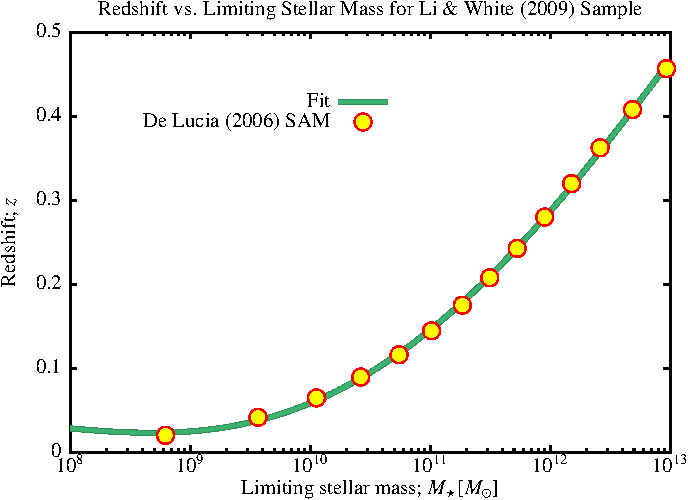
\includegraphics[width=85mm,trim=0mm 0mm 0mm 4mm,clip]{Plots/DataAnalysis/SDSSMassLuminosityRelation.pdf}
 \end{center}
 \caption{The maximum redshift at which a galaxy of given stellar mass can be detected in the sample of \protect\cite{li_distribution_2009}. Points show the results obtained using the \protect\cite{de_lucia_hierarchical_2007} model from the Millennium Database, while the lines shows a polynomial fit to these results (given in eqn.~\ref{eq:DepthPolynomial}).}
 \label{fig:SDSSDepthFit}
\end{figure}

\subsection{Bernardi et al. (2013)}\label{phys:surveyGeometry:surveyGeometryBernardi2013SDSS}

Selected with {\normalfont \ttfamily surveyGeometryMethod}$=${\normalfont \ttfamily bernardi2013SDSS}, this method describes the survey geometry of \cite{bernardi_massive_2013}. 

For the angular mask, we make use of the \gls{mangle} polygon file provided by the \gls{mangle} project\footnote{Specifically, \href{http://space.mit.edu/~molly/mangle/download/data/sdss_dr72safe0_res6d.pol.gz}{http://space.mit.edu/~molly/mangle/download/data/sdss\_dr72safe0\_res6d.pol.gz}.} The solid angle of this mask, computed using the \gls{mangle} {\normalfont \ttfamily harmonize} command is 2.232262776405~sr.

To determine the depth as a function of stellar mass, we make use of results provided by M. Bernardi (private communication), giving the mean maximum volume, $V_{\mathrm max}$, as a function of stellar mass for galaxies in this sample. These maximum volumes are converted to maximum distances using the solid angle quoted above. The results mass vs. distance relation is fit with a $5^{\mathrm th}$-order polynomial. Figure~\ref{fig:BernardiSDSSDepthFit} shows the resulting relation between stellar mass and the maximum distance at which such a galaxy would be included in the sample. Points indicate results from Bernardi, while the line shows a polynomial fit:
\begin{equation}
 \log_{10} \left[ {D_{\mathrm max}(M_\star) \over \hbox{Mpc}}\right] = 1282.11+m (-626.644+m (122.091+m (-11.8431+m (0.572399+m (-0.0110301)))))
 \label{eq:BernardiDepthPolynomial}
\end{equation}
where $m= \log_{10}(M_\star/M_\odot)$. We use this polynomial fit to determine the depth of the sample as a function of stellar mass.

\begin{figure}
 \begin{center}
 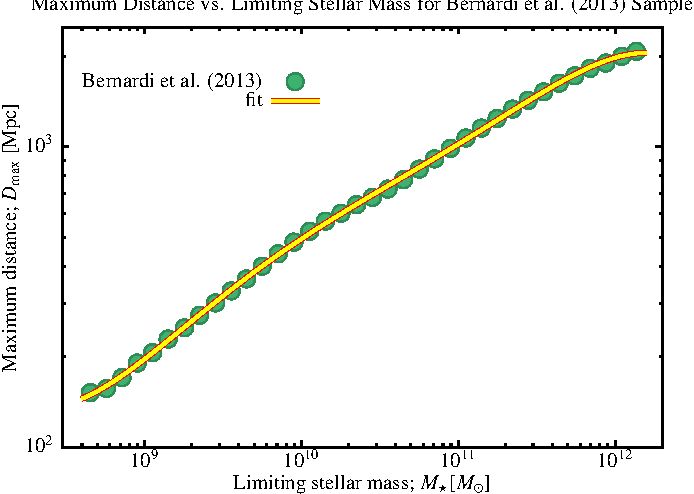
\includegraphics[width=85mm,trim=0mm 0mm 0mm 4mm,clip]{Plots/DataAnalysis/BernardiSDSSMassLuminosityRelation.pdf}
 \end{center}
 \caption{The maximum distance at which a galaxy of given stellar mass can be detected in the sample of \protect\cite{bernardi_massive_2013}. Points show the results obtained from data provided by Bernardi, while the lines shows a polynomial fit to these results (given in eqn.~\ref{eq:BernardiDepthPolynomial}).}
 \label{fig:BernardiSDSSDepthFit}
\end{figure}

\subsection{Davidzon et al. (2013)}\label{phys:surveyGeometry:surveyGeometryDavidzon2013VIPERS}

Selected with {\normalfont \ttfamily surveyGeometryMethod}$=${\normalfont \ttfamily davidzon2013VIPERS}, this method describes the survey geometry of \cite{davidzon_vimos_2013}. 

For the angular mask, we make use of {\normalfont \ttfamily mangle} polygon files provided by I.~Davidzon (private communication) corresponding to the VIPERS fields. The solid angle of each mask is computed using the {\normalfont \ttfamily mangle} {\normalfont \ttfamily harmonize} command.

To determine the depth as a function of stellar mass, we make use of the tabulated mass function, $\phi$, and number of galaxies per bin, $N$, supplied by I.~Davidzon (private communication). The effective volume of each bin is found as $V_i = N_i/f_{\mathrm complete}\phi_i\Delta\log_{10}M_\star$, where $\Delta\log_{10}M_\star$ is the width of the bin, and $f_{\mathrm complete}$ is the completeness of the survey, estimated to be approximately 40\% \citep{guzzo_vimos_2013}. These volumes are converted to maximum distances in each field using the survey solid angle. The resulting mass vs. distance relation in each field is fit with a $1^{\mathrm st}$-order polynomial in log-log space over the range where the maximum volume is limited by the survey depth and not by the imposed upper limit to redshift. Figure~\ref{fig:Davidzon2013DepthFit} shows the resulting relation between stellar mass and the maximum distance at which such a galaxy would be included in the sample. Points indicate results from VIPERS, while the lines show polynomial fits:
\begin{equation}
 \log_{10} \left[ {D_{\mathrm max}(M_\star) \over \hbox{Mpc}}\right] = \left\{ \begin{array}{ll} 3.207 + 0.0124m & 0.5 < z < 0.6 \\ 3.148 + 0.0268m & 0.6 < z < 0.8  \\ 3.207 + 0.0273m & 0.8 < z < 1.0 \end{array} \right.
 \label{eq:DavidzonDepthPolynomial}
\end{equation}
where $m= \log_{10}(M_\star/M_\odot)$. We use this polynomial fit to determine the depth of the sample as a function of stellar mass.

\begin{figure}
 \begin{center}
 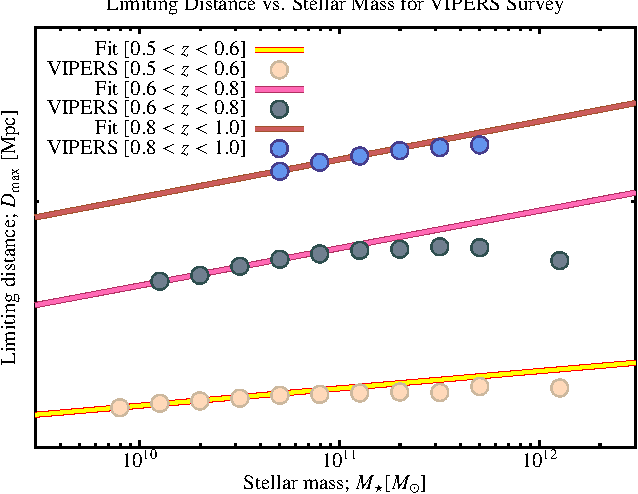
\includegraphics[width=85mm,trim=0mm 0mm 0mm 4mm,clip]{Plots/DataAnalysis/DavidzonVIPERSMassDistanceRelation.pdf}
 \end{center}
 \caption{The maximum distance at which a galaxy of given stellar mass can be detected in the sample of \protect\cite{davidzon_vimos_2013}. Points show the results obtained from data provided by Davidzon, while the lines shows a polynomial fit to these results (given in eqn.~\ref{eq:DavidzonDepthPolynomial}). Note that at high masses the distance is limited by the imposed upper limit---the polynomial fit does not consider these points.}
 \label{fig:Davidzon2013DepthFit}
\end{figure}

\subsection{Tomczak et al. (2014)}\label{phys:surveyGeometry:surveyGeometryTomczak2014ZFOURGE}

Selected with {\normalfont \ttfamily surveyGeometryMethod}$=${\normalfont \ttfamily tomczak2014ZFOURGE}, this method describes the survey geometry of \cite{tomczak_galaxy_2014}. 

For the angular mask, we make use of {\normalfont \ttfamily mangle} polygon files constructed by hand using vertices matched approximately to the distribution of galaxies in the survey (positions of which were provided by R.~Quadri; private communication). The solid angle of each mask is computed using the {\normalfont \ttfamily mangle} {\normalfont \ttfamily harmonize} command.

To determine the depth as a function of stellar mass, we make use of the tabulated mass completeness limits as a function of redshift for ZFOURGE and NMBS fields provided by R.~Quadri (private communication). These are fit with fourth-order polynomials. Figure~\ref{fig:Tomczak2014DepthFit} shows the resulting relation between stellar mass and the maximum redshift at which such a galaxy would be included in the sample. Dotted lines indicate the tabulated result from ZFOURGE, while the lines show polynomial fits:
\begin{equation}
 z_{\mathrm max}(M_\star) = \left\{ \begin{array}{ll} -114.66+m*(45.901+m*(-6.1617+m*(0.27822))) & \hbox{ZFOURGE fields} \\ -58.483+m*(20.250+m*(-2.3563+m*(0.092705))) & \hbox{NMBS fields} \end{array} \right.
 \label{eq:TomczakDepthPolynomial}
\end{equation}
where $m= \log_{10}(M_\star/M_\odot)$. We use this polynomial fit to determine the depth of the sample as a function of stellar mass.

\begin{figure}
 \begin{center}
 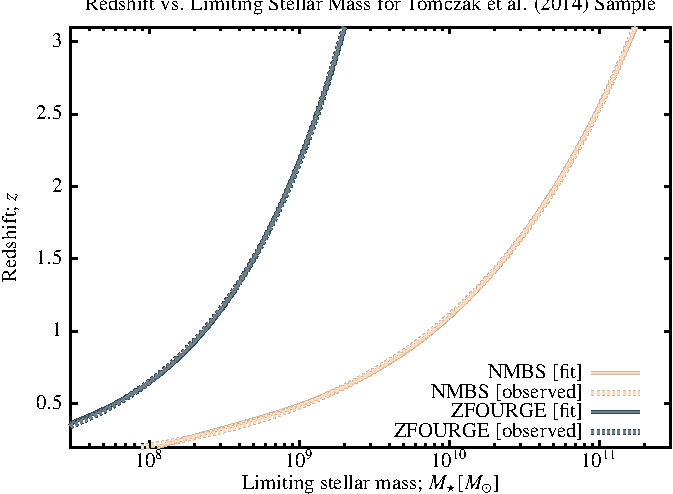
\includegraphics[width=85mm,trim=0mm 0mm 0mm 4mm,clip]{Plots/DataAnalysis/TomczakZFOURGEMassRedshiftRelation.pdf}
 \end{center}
 \caption{The maximum redshift at which a galaxy of given stellar mass can be detected in the sample of \protect\cite{tomczak_galaxy_2014}. Points show the results obtained from data provided by Davidzon, while the lines shows a polynomial fit to these results (given in eqn.~\ref{eq:TomczakDepthPolynomial}).}
 \label{fig:Tomczak2014DepthFit}
\end{figure}

\subsection{Baldry et al. (2012)}\label{phys:surveyGeometry:surveyGeometryBaldry2012GAMA}

Selected with {\normalfont \ttfamily surveyGeometryMethod}$=${\normalfont \ttfamily baldry2012GAMA}, this method describes the survey geometry of \cite{baldry_galaxy_2012}. 

For the angular mask we use the specifications of the G09, G12, and G15 fields given by \cite{driver_galaxy_2011} to construct {\normalfont \scshape mangle} polygon files.

To determine the depth as a function of stellar mass, we make use of the publicly available tabulated mass function, $\phi$, and number of galaxies per bin, $N$. The effective volume of each bin is found as $V_i = N_i/\phi_i\Delta\log_{10}M_\star$, where $\Delta\log_{10}M_\star$ is the width of the bin. The GAMA survey consists of three fields, each of the same solid angle, but with differing depths. We assume that the relative depths in terms of stellar mass scale with the depth in terms of flux. Given this assumption, these volumes are converted to maximum distances in each field using the solid angle quoted above. The resulting mass vs. distance relation in each field is fit with a $1^{\mathrm st}$-order polynomial in log-log space over the range where the maximum volume is limited by the survey depth and not by the imposed $z=0.06$ upper limit to redshift. Figure~\ref{fig:BaldryGAMADepthFit} shows the resulting relation between stellar mass and the maximum distance at which such a galaxy would be included in the sample. Points indicate results from GAMA, while the line shows a polynomial fit:
\begin{equation}
 \log_{10} \left[ {D_{\mathrm max}(M_\star) \over \hbox{Mpc}}\right] = \left\{ \begin{array}{ll} -0.521 + 0.319m & \hbox{fields G09/G15} \\ -0.361 + 0.319m & \hbox{field G12} \end{array} \right.
 \label{eq:BaldryDepthPolynomial}
\end{equation}
where $m= \log_{10}(M_\star/M_\odot)$. We use this polynomial fit to determine the depth of the sample as a function of stellar mass.

\begin{figure}
 \begin{center}
 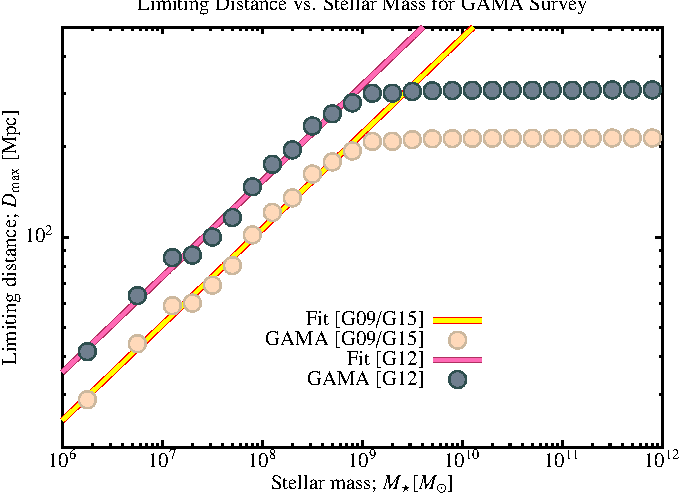
\includegraphics[width=85mm,trim=0mm 0mm 0mm 4mm,clip]{Plots/DataAnalysis/BaldryGAMAMassDistanceRelation.pdf}
 \end{center}
 \caption{The maximum distance at which a galaxy of given stellar mass can be detected in the sample of \protect\cite{baldry_galaxy_2012}. Points show the results obtained from data provided by Baldry, while the lines shows a polynomial fit to these results (given in eqn.~\ref{eq:BaldryDepthPolynomial}). Note that above $10^9M_\odot$ the distance is limited by the imposed upper limit of $z=0.06$ in the GAMA sample---the polynomial fit does not consider these points.}
 \label{fig:BaldryGAMADepthFit}
\end{figure}

\subsection{Moustakas et al. (2013)}\label{phys:surveyGeometry:surveyGeometryMoustakas2013PRIMUS}

Selected with {\normalfont \ttfamily surveyGeometryMethod}$=${\normalfont \ttfamily moustakas2013PRIMUS}, this method describes the survey geometry of \cite{moustakas_primus:_2013}. 

For the angular mask, we make use of \gls{mangle} polygon files provided by J.~Moustakas (private communication)  corresponding to the give PRIMUS fields. The solid angle of each mask is computed using the \gls{mangle} {\normalfont \ttfamily harmonize} command.

To determine the depth as a function of stellar mass, we make use of completeness limits for ``All'' galaxies given in Table~2 of \cite{moustakas_primus:_2013}. These are fit, for each field with a second order polynomial to give the limiting redshift as a function of stellar mass. Figure~\ref{fig:MoustakasPRIMUSDepthFit} shows the resulting relation between stellar mass and the maximum redshift at which such a galaxy would be included in the sample. Points indicate results from \cite{moustakas_primus:_2013}, while the line shows a polynomial fits:
\begin{eqnarray}
z_{\mathrm max}(M_\star) = +3.51+m(-0.941+m(+0.0651)) & & \hbox{COSMOS} \\
z_{\mathrm max}(M_\star) = +2.46+m(-0.730+m(+0.0542)) & & \hbox{XMM-SXDS} \\
z_{\mathrm max}(M_\star) = -3.60+m(+0.500+m(-0.0078)) & & \hbox{XMM-CFHTLS} \\
z_{\mathrm max}(M_\star) = +5.87+m(-1.528+m(+0.0982)) & & \hbox{CDFS} \\
z_{\mathrm max}(M_\star) = +6.87+m(-1.656+m(+0.1003)) & & \hbox{ELAIS-S1}
 \label{eq:MoustakasDepthPolynomial}
\end{eqnarray}
where $m= \log_{10}(M_\star/M_\odot)$. We use this polynomial fit to determine the depth of the sample as a function of stellar mass.

\begin{figure}
 \begin{center}
 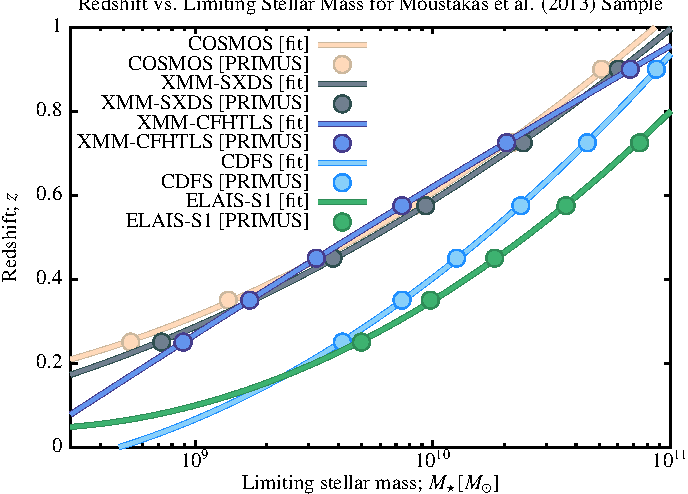
\includegraphics[width=85mm,trim=0mm 0mm 0mm 4mm,clip]{Plots/DataAnalysis/MoustakasPRIMUSMassRedshiftRelation.pdf}
 \end{center}
 \caption{The maximum distance at which a galaxy of given stellar mass can be detected in the sample of \protect\cite{moustakas_primus:_2013}. Points show the results obtained from completeness limit data taken from Table~2 of \protect\cite{moustakas_primus:_2013}, while the lines shows a polynomial fit to these results (given in eqn.~\ref{eq:MoustakasDepthPolynomial}).}
 \label{fig:MoustakasPRIMUSDepthFit}
\end{figure}

\subsection{Muzzin et al. (2013)}\label{phys:surveyGeometry:surveyGeometryMuzzin2014ULTRAVISTA}

Selected with {\normalfont \ttfamily surveyGeometryMethod}$=${\normalfont \ttfamily muzzin2013ULTRAVISTA}, this method describes the survey geometry of \cite{muzzin_evolution_2013}. 

For the angular mask, we generate a \gls{mangle} polygon file, by first defining a rectangle encompassing the bounds of the ULTAVISTA field ($149.373^\circ < \alpha < 150.779^\circ$ and $1.604^\circ < \delta < 2.81^\circ$). From this rectangle, we then remove circles of radii $75^{\prime\prime}$ around bright stars (i.e. those bright than 10$^{\mathrm th}$ and $8^{\mathrm th}$ magnitudes in the USNO and 2MASS star lists respectively) and radii $30^{\prime\prime}$ around medium stars (i.e. those bright than $13^{\mathrm th}$ and $10.5^{\mathrm th}$ magnitudes in the USNO and 2MASS star lists respectively). Finally, we mask regions of one detector for which 75\% of pixels are dead by clipping pixels with weights below $0.02$ in the K$_{\mathrm s}$-band weight map. These choices match those made in the ULTRAVISTA survey (A.~Muzzin, private communication). The solid angle of each mask is computed using the \gls{mangle} {\normalfont \ttfamily harmonize} command.

To determine the depth as a function of stellar mass, we simply fit the \href{http://www.strw.leidenuniv.nl/galaxyevolution/ULTRAVISTA/Mstar_redshift_completeness_emp_uvista_v4.1_100.dat}{tabulated relations} provided by the ULTRAVISTA survey:
\begin{equation}
z_{\mathrm max}(M_\star) = {-8364.45 + m (4331.82 + m (-896.596 + m (92.6999 + m (-4.78750 + m (0.0988215))))) \over 1 - \exp[(m-11.24)/0.02] }
 \label{eq:MuzzinDepthPolynomial}
\end{equation}
where $m= \log_{10}(M_\star/M_\odot)$.

\begin{figure}
 \begin{center}
 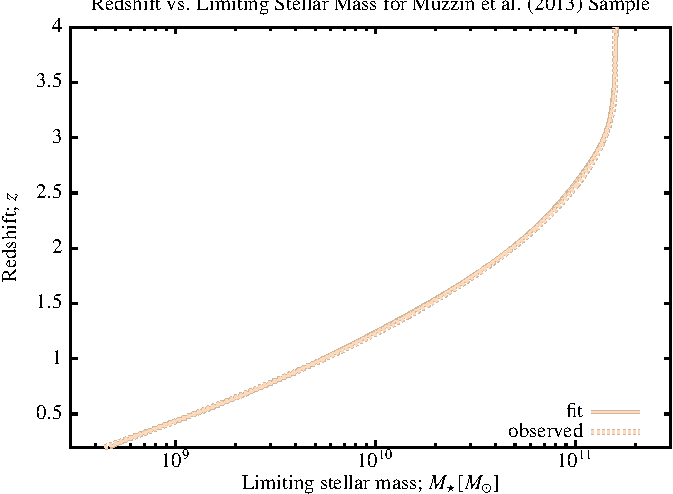
\includegraphics[width=85mm,trim=0mm 0mm 0mm 4mm,clip]{Plots/DataAnalysis/MuzzinULTRAVISTAMassRedshiftRelation.pdf}
 \end{center}
 \caption{The maximum distance at which a galaxy of given stellar mass can be detected in the sample of \protect\cite{muzzin_evolution_2013}. The dotted line shows the results obtained from the ULTRAVISTA survey \protect\citep{muzzin_evolution_2013}, while the solid line shows the polynomial fit to these results (given in eqn.~\ref{eq:MuzzinDepthPolynomial}).}
 \label{fig:MuzzinULTRAVISTADepthFit}
\end{figure}

\subsection{Martin et al. (2010)}\label{phys:surveyGeometry:surveyGeometryMartin2010ALFALFA}

Selected with {\normalfont \ttfamily surveyGeometryMethod}$=${\normalfont \ttfamily martin2010ALFALFA}, this method describes the survey geometry of \cite{martin_arecibo_2010}. 

For the angular mask we use the three disjoint regions defined by 07$^{\mathrm h}$30$^{\mathrm m}$ $<$ R.A. $<$ 16$^{\mathrm h}$30$^{\mathrm m}$, +04$^\circ$ $<$ decl. $<$ +16$^\circ$, and +24$^\circ$ $<$ decl. $<$ +28$^\circ$ and 22$^{\mathrm h}$ $<$ R.A. $<$ 03$^{\mathrm h}$, +14$^\circ$ $<$ decl. $<$ +16$^\circ$, and +24$^\circ$ $<$ decl. $<$ +32$^\circ$ corresponding to the sample of \cite{martin_arecibo_2010}. When the survey window function is needed we generate randomly distributed points within this angular mask and out to the survey depth. These points are used to determine which elements of a 3D grid fall within the window function.

To estimate the depth of the \cite{martin_arecibo_2010} sample as a function of galaxy HI mass we first infer the median line width corresponding to that mass. To do so, we have fit the median line width-mass relation from the $\alpha.40$ sample with power-law function as shown in Fig.~\ref{fig:ALFALFALineWidthMassRelation}. We find that the median line width can be approximated by
\begin{equation}
 \log_{10} (W_{\mathrm 50}/\hbox{km s}^{-1}) = c_0 + c_1 \log_10(M_{\mathrm HI}/M_\odot),
 \label{eq:ALFALFALineWidthMassRelation}
\end{equation}
with $c_0=-0.770$ and $c_1=0.315$. Given the line width, the corresponding integrated flux limit, $S_{\mathrm int}$, for a signal-to-noise of $6.5$ is inferred using equation~(A1) of \cite{haynes_arecibo_2011}. Finally, this integrated flux limit is converted to maximum distance at which the source could be detected using the expression given in the text of section~2.2 of \cite{martin_arecibo_2010}:
\begin{equation}
 M_{\mathrm HI} = 2.356\times10^5 \left({D\over \hbox{Mpc}}\right)^2 \left({S_{\mathrm int}\over\hbox{Jy km s}^{-1}}\right).
\end{equation}

\begin{figure}
 \begin{center}
  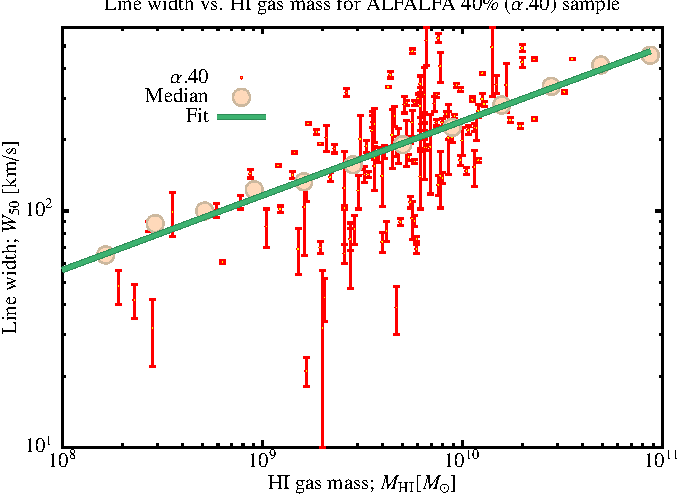
\includegraphics[width=85mm,trim=0mm 0mm 0mm 4mm,clip]{Plots/DataAnalysis/alfalfaHILineWidthMassRelation.pdf}
 \end{center}
 \caption{HI line width vs. HI mass as measured from the $\alpha.40$ survey of \protect\cite{martin_arecibo_2010}. Red points with error bars show individual measurements, while the larger circles indicate the running median of these data. The green line is a power-law fit to the running median as described in eqn.~(\protect\ref{eq:ALFALFALineWidthMassRelation}).}
 \label{fig:ALFALFALineWidthMassRelation}
\end{figure}

\subsection{Caputi et al. (2011)}\label{phys:surveyGeometry:surveyGeometryCaputi2011UKIDSSUDS}

Selected with {\normalfont \ttfamily surveyGeometryMethod}$=${\normalfont \ttfamily caputi2011UKIDSSUDS}, this method describes the survey geometry of \cite{caputi_stellar_2011}. 

The angular mask is defined by the boundaries given in Table~\ref{tb:CaputiSurveyBoundaries} together with a set of rectangular holes fitted to gaps in the galaxy distribution provided by Karina Caputi (private communication). In particular, a set of points randomly distributed in the survey mask is constructed by the script {\normalfont \ttfamily constraints/dataAnalysis/stellarMassFunctions\_UKIDSS\_UDS\_z3\_5/surveyGeometryRandoms.pl}. These points are used to determine which elements of a 3D grid fall within the window function. We compute a solid angle of $1.592\times 10^{-4}$~sr for the sample from this window function.

\begin{table}
\caption{Boundaries of the angular mask for the survey of \protect\cite{caputi_stellar_2011}. Each boundary consists of a great circle segment defined by start and end coordinates (given in tuples of right acesension and declination in units of degrees), together with a ``type'' which specifies whether points above, below, to the right or left of the boundary are part of the survey (where ``above'' and ``below'' refer to declination, and ``left'' and ``right'' refer to right acsension).}
\label{tb:CaputiSurveyBoundaries}
\begin{center}
\begin{tabular}{@{(}r@{,}l@{)\;(}r@{,}l@{)\;}l}
\hline
\multicolumn{2}{c}{\normalfont \bfseries Start} & \multicolumn{2}{c}{\normalfont \bfseries End} & {\normalfont \bfseries Type} \\
\hline
 34.460 & -4.648 & 34.750 & -4.648 & above \\
 34.000 & -4.908 & 34.460 & -4.648 & above \\
 34.900 & -4.920 & 34.750 & -4.648 & above \\
 34.440 & -5.518 & 34.905 & -5.255 & below \\
 34.210 & -5.518 & 34.440 & -5.518 & below \\
 34.210 & -5.518 & 34.000 & -5.150 & below \\
 34.000 & -4.908 & 34.000 & -5.150 & left  \\
 34.900 & -4.920 & 34.905 & -5.255 & right \\
\hline
\end{tabular}
\end{center}
\end{table}

To estimate the depth of the \cite{caputi_stellar_2011} sample as a function of galaxy stellar mass we make use of semi-analytic models in the Millennium Database. Specifically, we use the \glspl{sam} of \cite{henriques_confronting_2012} and \citeauthor{guo_dwarf_2011}~(\citeyear{guo_dwarf_2011}; specifically the {\normalfont \ttfamily Henriques2012a.wmap1.BC03\_001} and {\normalfont \ttfamily Guo2010a..MR} tables in the Millennium Database). For each snapshot in the database, we extract the stellar masses and observed-frame IRAC $4.5\mu$m apparent magnitudes (including dust extinction), and determine the median apparent magnitude as a function of stellar mass. Using the limiting apparent magnitude of the \cite{caputi_stellar_2011} sample, $24.0$, we infer the corresponding stellar mass.

The end result of this procedure is the limiting stellar mass as a function of redshift, accounting for k-corrections, evolution, and the effects of dust. Figure~\ref{fig:UKIDSSUDSDepthFit} shows the resulting relation between stellar mass and the maximum redshift at which such a galaxy would be included in the sample. Points indicate measurements from the \gls{sam}, while the line shows a polynomial fit:
\begin{eqnarray}
 z(M_\star) &=& -56.247 + 5.881 \log_{10}(M_\star/M_\odot).
 \label{eq:UKIDSSDepthPolynomial}
\end{eqnarray}
We use this polynomial fit to determine the depth of the sample as a function of stellar mass.

\begin{figure}
 \begin{center}
 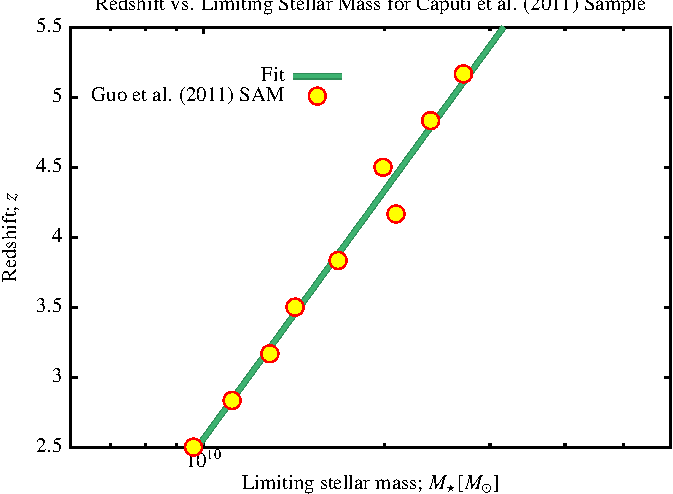
\includegraphics[width=85mm,trim=0mm 0mm 0mm 4mm,clip]{Plots/DataAnalysis/UKIDSSUDSMassLuminosityRelation.pdf}
 \end{center}
 \caption{The maximum redshift at which a galaxy of given stellar mass can be detected in the sample of \protect\cite{caputi_stellar_2011}. Points show the results obtained using the \protect\cite{henriques_confronting_2012} and \protect\cite{guo_dwarf_2011} models from the Millennium Database, while the lines shows a polynomial fit to these results (given in eqn.~\ref{eq:UKIDSSDepthPolynomial}).}
 \label{fig:UKIDSSUDSDepthFit}
\end{figure}
